\documentclass[landscape]{article}
\usepackage[a4paper,margin=1.1cm,footskip=0.6cm]{geometry}
\usepackage[utf8]{inputenc}
\usepackage[T1]{fontenc}
\usepackage{multicol}
\usepackage{multirow}
\usepackage{lipsum}
\usepackage{makecell}
\usepackage{amsmath}
\usepackage{amssymb}
\usepackage{algpseudocode}
\usepackage{algorithmicx}
\usepackage{color}
\usepackage[table]{xcolor}
\usepackage{tikz}
\usepackage{listings}
\usepackage{tocloft}
\usepackage[hidelinks]{hyperref}

% Define new colors
\definecolor{cgreen}{RGB}{0, 100, 0}
\definecolor{clime}{RGB}{120, 210, 0}
\definecolor{corange}{RGB}{255, 165, 0}
\definecolor{cred}{RGB}{215, 20, 20}
\definecolor{cpurple}{RGB}{160, 32, 240}
\definecolor{sky}{RGB}{90, 120, 190}

% Define a new list of methods
\newlistof{methods}{mtd}{Reference}

\lstset{
    language=C++,
    keywordstyle=\bfseries,
    basicstyle=\ttfamily,
    columns=fullflexible,
    aboveskip=0em,
    belowskip=0.5em,
    breaklines=true,
    breakindent=2.5em
}


% blue for \Function name
\let\oldFunction\Function
\renewcommand{\Function}[2]{\oldFunction{\textcolor{sky}{#1}}{#2}}
\let\oldComment\Comment
\renewcommand{\Comment}[1]{\oldComment{\textcolor{gray}{#1}}}

\definecolor{algkw}{RGB}{20, 60, 130}

\newcommand{\True}{\textbf{True}}
\newcommand{\False}{\textbf{False}}
\newcommand{\Break}{\State \textbf{\textcolor{algkw}{break}}}
\newcommand{\algkw}[1]{\textbf{\textcolor{algkw}{#1}}}
\algrenewcommand\algorithmicfunction{\textbf{\color{algkw}function}}
\algrenewcommand\algorithmicend{\textbf{\color{algkw}end}}
\algrenewcommand\algorithmicif{\textbf{\color{algkw}if}}
\algrenewcommand\algorithmicthen{\textbf{\color{algkw}then}}
\algrenewcommand\algorithmicelse{\textbf{\color{algkw}else}}
\algrenewcommand\algorithmicfor{\textbf{\color{algkw}for}}
\algrenewcommand\algorithmicwhile{\textbf{\color{algkw}while}}
\algrenewcommand\algorithmicdo{\textbf{\color{algkw}do}}
\algrenewcommand\algorithmicrepeat{\textbf{\color{algkw}repeat}}
\algrenewcommand\algorithmicuntil{\textbf{\color{algkw}until}}
\algrenewcommand\algorithmicreturn{\textbf{\color{algkw}return}}


\usepackage{graphicx}
\graphicspath{ {./images/} }

\setlength{\columnsep}{1cm}
\renewcommand{\columnseprulecolor}{\normalcolor}
% set \paragraph vertical spacing
\makeatletter
\renewcommand{\paragraph}{\@startsection{paragraph}{4}{\z@}%
                                    {1.5ex}%
                                    {-0.75em}%
                                    {\normalfont\normalsize\bfseries}}
\makeatother
% reduce space before \subparagraph
\makeatletter
\renewcommand{\subparagraph}{\@startsection{subparagraph}{5}{\z@}%
                                       {1ex}%
                                       {-0.75em}%
                                       {\normalfont\small\bfseries\hspace{1.25em}}}% Add \hspace{1.25em} for 1 level of indent
\makeatother
% add vertical space before \minipage and rename environment to \minipage
\let\oldminipage\minipage
\let\endoldminipage\endminipage
\renewenvironment{minipage}{\vspace{0.5em}\begin{oldminipage}{\linewidth}}{\end{oldminipage}}

% Custom command for horizontal separator
\newcommand{\sep}{\noindent\rule{\linewidth}{0.4pt}}

\newcommand{\sepdotted}{\noindent\makebox[\linewidth]{\dotfill}}

% Custom command for highlighting text
\newcommand{\highlight}[2][sky!30]{\setlength{\fboxsep}{0pt}\colorbox{#1}{#2}}

% \pagenumbering{gobble}

\begin{document}
\begin{multicols*}{3}
    \footnotesize % Change the font size here if needed
    \section*{ASD - Algorithmes et Structures de Données \\ \small{Leonard Cseres | Juin 2024}}
    \paragraph{Complexité}\mbox{}\\
    \scalebox{0.8}{
    \highlight[cgreen!30]{$\mathcal{O}(1)$} $<$ \highlight[clime!30]{$\mathcal{O}(\log(n))$} $<$ \highlight[corange!30]{$\mathcal{O}(n)$} $<$ \highlight[cred!30]{$\mathcal{O}(n\cdot\log(n))$} $<$ \highlight[cpurple!30]{$\mathcal{O}(n^c)$} $<$ \highlight[cpurple!30]{$\mathcal{O}(2^n)$} $<$ \highlight[cpurple!30]{$\mathcal{O}(n!)$} $<$ \highlight[cpurple!30]{$\mathcal{O}(n^n)$}
        }
        \sepdotted
        \begin{algorithmic}
            \For{$i = 1$ \algkw{to} $n$ \algkw{step} \highlight{$i \times \alpha$}} \Comment{$\mathcal{O}(\log_\alpha(n))$}
                \State $k \gets k + 1$
            \EndFor
        \end{algorithmic}
        \sepdotted
        \begin{algorithmic}
            \For{$i = 1$ \algkw{to} $n$ \algkw{step} \highlight{$i \times i$}} \Comment{$\mathcal{O}(\sqrt{n})$}
            \State $k \gets k + 1$
            \EndFor
        \end{algorithmic}
        \sepdotted
        \begin{algorithmic}
            \For{$i = 0$ \algkw{to} $n$} \Comment{$\mathcal{O}(n\cdot\frac{(n-1)}{2})$}
            \For{$j = 0$ \highlight{\algkw{to} $i$}}
            \State $k \gets k + 1$
            \EndFor
            \EndFor
        \end{algorithmic}
        \sepdotted
        \begin{algorithmic}
            \For{$i = 0$ \highlight{\algkw{to} $n$ \algkw{and} $m$}} \Comment{$\mathcal{O}(min(n, m))$}
                \State $k \gets k + 1$
            \EndFor
        \end{algorithmic}
        \sepdotted
        \begin{algorithmic}
            \For{$i = 0$ \highlight{\algkw{to} $n$ \algkw{or} $m$}} \Comment{$\mathcal{O}(max(n, m))$}
                \State $k \gets k + 1$
            \EndFor
        \end{algorithmic}\mbox{}\\

        \paragraph{Cas spéciaux}\mbox{}\vspace*{0.5em}
        \par\noindent\begin{minipage}
            \centering
            \begin{tabular}[h]{l|l}
                \textbf{Operation}                                               & \textbf{Complexité}                     \\
                \hline
                \texttt{rand()} \% $n == 0$                                      & \cellcolor{corange!30}$P = \frac{1}{n}$ \\
                (\texttt{rand()} \% $n$) $\cdot$ (\texttt{rand()} \% $n$) $== n$ & \cellcolor{corange!30}$P = \sqrt{n}$    \\
            \end{tabular}
        \end{minipage}

        \paragraph{Récursivité} $C = \text{nb\_appels\_rec}^\text{profondeur}$\vspace*{0.5em}
        
        \noindent\begin{minipage}
            \centering
            \begin{tabular}{l|l}
                \textbf{Algorithmes}    & \textbf{Complexités}                                                      \\
                \hline
                Factorielle récursif    & \cellcolor{corange!30}$\mathcal{O}(n)$                                    \\
                Factorielle itératif    & \cellcolor{corange!30}$\mathcal{O}(n)$                                    \\
                Fibonacci récursif      & \cellcolor{cpurple!30}$\mathcal{O}(\phi^n),\ \phi = \frac{\sqrt{5}+1}{2}$ \\
                Fibonacci itératif      & \cellcolor{corange!30}$\mathcal{O}(n)$                                    \\
                PGCD (Euclide)          & \cellcolor{clime!30}$\mathcal{O}(\log(n))$                                \\
                Tours de Hanoï récursif & \cellcolor{cpurple!30}$\mathcal{O}(2^n)$                                  \\
                Tours de Hanoï itératif & \cellcolor{cpurple!30}$\mathcal{O}(2^n)$                                  \\
                Permutations            & \cellcolor{cpurple!30}$\mathcal{O}(n!)$                                   \\
                Tic Tac Toe             & \cellcolor{cgreen!30}$9!$                                                 \\
                \makecell[l]{Puissance 4                                                                            \\(Profondeur d’exploration de $d$ tours)}                             & \cellcolor{cpurple!30}$\mathcal{O}(7^d)$             \\
                \makecell[l]{Minimax (negamax)                                                                      \\(M mouvements possibles par tour,\\profondeur de $d$ tours)}                       & \cellcolor{cpurple!30}$\mathcal{O}(m \cdot d)$       \\
            \end{tabular}
        \end{minipage}\\

        \columnbreak

        \paragraph{Algorithmes de Tri}\mbox{}\vspace{0.5em}\\
        \scalebox{0.705}{
            \begin{tabular}[h]{l|l|l|l|l|l}
                \textbf{Algorithme} & \textbf{Pire cas}                              & \textbf{Moyen}                           & \textbf{Meilleur}                        & \textbf{Stable} & \textbf{En place} \\
                \hline
                Tri à bulles        & \cellcolor{cpurple!30}$\mathcal{O}(n^2)$       & \cellcolor{cpurple!30}$\Theta(n^2)$      & \cellcolor{corange!30}$\Omega(n)$        & Oui ($\leq$)    & Oui               \\
                Tri par sélection   & \cellcolor{cpurple!30}$\mathcal{O}(n^2)$       & \cellcolor{cpurple!30}$\Theta(n^2)$      & \cellcolor{cpurple!30}$\Omega(n^2)$      & Non             & Oui               \\
                Tri par insertion   & \cellcolor{cpurple!30}$\mathcal{O}(n^2)$       & \cellcolor{cpurple!30}$\Theta(n^2)$      & \cellcolor{corange!30}$\Omega(n)$        & Oui             & Oui               \\
                Tri fusion          & \cellcolor{cred!30}$\mathcal{O}(n\log(n))$     & \cellcolor{cred!30}$\Theta(n\log(n))$    & \cellcolor{cred!30}$\Omega(n\log(n))$    & Oui             & Non               \\
                Tri rapide          & \cellcolor{cpurple!30}$\mathcal{O}(n^2)$       & \cellcolor{cred!30}$\Theta(n\log(n))$    & \cellcolor{cred!30}$\Omega(n\log(n))$    & Non             & Oui               \\
                Tri comptage        & \cellcolor{corange!30}$\mathcal{O}(n+k)$       & \cellcolor{corange!30}$\Theta(n+k)$      & \cellcolor{corange!30}$\Omega(n+k)$      & Oui             & Non               \\
                Tri par base        & \cellcolor{corange!30}$\mathcal{O}(n\cdot  k)$ & \cellcolor{corange!30}$\Theta(n\cdot k)$ & \cellcolor{corange!30}$\Omega(n\cdot k)$ & Oui             & Non               \\
                Selection rapide    & \cellcolor{cpurple!30}$\mathcal{O}(n^2)$       & \cellcolor{corange!30}$\Theta(n)$        & \cellcolor{corange!30}$\Omega(n)$        & Non             & Oui               \\
            \end{tabular}
        }\\

        \noindent\lstinline[basicstyle=\ttfamily\color{cred}]{void qsort(start, count, size, cmp)}\\
    $\Theta(n\log(n))$, $\mathcal{O}(n^2)$, pas stable (\texttt{<cstdlib>})\\

        \noindent\lstinline[basicstyle=\ttfamily\color{cred}]{void sort(first, last, cmp)}\\
    $\Theta(n\log(n))$, \texttt{swap} à implémenter\\

        \noindent\lstinline[basicstyle=\ttfamily\color{cred}]{void stable_sort(first, last, cmp)}\\
    $\mathcal{O}(n\log(n))$, $\mathcal{O}(n\log^2(n))$ si fait en place et doit utiliser $< >$ pour la stabilité (tri fusion)\\

        \noindent\lstinline[basicstyle=\ttfamily\color{corange}]{void nth_element(first, nth, last)}\\
    $\mathcal{O}(n)$, où $n = \texttt{last} - \texttt{first}$\\

        \noindent\lstinline[basicstyle=\ttfamily\color{cred}]{void partial_sort(first, middle, last)}\\
    $\mathcal{O}(n\log(m))$, où $n = \texttt{last} - \texttt{first}$ et $m = \texttt{middle} - \texttt{first}$

        \sep
        \paragraph{Structures linéaires}\mbox{}\vspace{0.5em}\\
        \scalebox{0.9}{
            \begin{tabular}{l|l}
                \hline
                \textit{Sequence}              &                                                 \\
                \hline
                \texttt{array, vector}         &                                                 \\
                \texttt{deque}                 & Double-ended queue                              \\
                \texttt{forward\_list}         & Liste chaînée simple                            \\
                \texttt{list}                  & Liste chaînée double                            \\
                \hline
                \textit{Adaptative}            &                                                 \\
                \hline
                \texttt{stack}                 & Pile (LIFO)                                     \\
                \texttt{queue}                 & File (FIFO)                                     \\
                \texttt{priority\_queue}       & File de priorité                                \\
                \hline
                \textit{Associative}           & \textcolor{gray}{\textit{Balanced Binary Tree}} \\
                \hline
                \texttt{set}                   & Ensemble trié                                   \\
                \texttt{multiset}              & Ensemble trié avec doublons                     \\
                \texttt{map}                   & Table de hachage                                \\
                \texttt{multimap}              & Table de hachage avec doublons                  \\
                \hline
                \textit{Unordered associative} & \textcolor{gray}{\textit{Hash Table}}           \\
                \hline
                \texttt{unordered\_set}        & Ensemble non trié                               \\
                \texttt{unordered\_multiset}   & Ensemble non trié avec doublons                 \\
                \texttt{unordered\_map}        & Table de hachage non triée                      \\
                \texttt{unordered\_multimap}   & Table de hachage non triée avec doublons
            \end{tabular}
        }

        \paragraph{Buffer Circulaire} {\tiny ($+$)} $\mathcal{O}(1)$ pour ajouter, supprimer et accéder, {\tiny ($-$)} $\mathcal{O}(\min(i, N - i))$ pour insérer ou supprimer à l'index $i$, {\tiny ($-$)} capacité fixe
        
        \paragraph{Deque}\mbox{}
        \par\noindent\begin{minipage}
            \centering
            \begin{tabular}{l|l}
                \textbf{Opération}           & \textbf{Complexité}                                 \\
                \hline
                Allouer un nouveau block             & \cellcolor{cgreen!30}$\mathcal{O}(B)$               \\
                Ré-allouer la map                    & \cellcolor{corange!30}$\mathcal{O}(n/B)$            \\
                Insertion                            & \cellcolor{corange!30}$\mathcal{O}(B + n/B)$        \\
                Insertion/suppression à l'indice $i$ & \cellcolor{corange!30}$\mathcal{O}(\min(i, n - i))$ \\
            \end{tabular}
        \end{minipage}\vspace{0.5em}\\

        \noindent\scalebox{0.675}{
            \begin{tabular}{l|c|c|c|c|c}
                                    & \texttt{array}                         & \texttt{vector}                                    & \texttt{forward\_list}                   & \texttt{list}                            & \texttt{deque}                                             \\
                \hline
                Mémoire extra       & \cellcolor{cgreen!30} 0                & \cellcolor{gray!30} $3p + \mathcal{O}(n) \cdot t$  & \cellcolor{gray!30} $p(n+1)$             & \cellcolor{gray!30} $p(2n + 3)$          & \cellcolor{gray!30} \makecell{$\mathcal{O}(n/B) \cdot p +$ \\$\mathcal{O}(B) \cdot t + 6p$} \\
                operator[]          & \cellcolor{cgreen!30} $\mathcal{O}(1)$ & \cellcolor{cgreen!30} $\mathcal{O}(1)$             & \cellcolor{cred!30} N/A                  & \cellcolor{cred!30} N/A                  & \cellcolor{cgreen!30} $\mathcal{O}(1)^2$                   \\
                push/pop front      & \cellcolor{cred!30} N/A                & \cellcolor{corange!30} $\mathcal{O}(n)$            & \cellcolor{cgreen!30} $\mathcal{O}(1)$   & \cellcolor{cgreen!30} $\mathcal{O}(1)$   & \cellcolor{cgreen!30} $\mathcal{O}(1)$                     \\
                insert/erase milieu & \cellcolor{cred!30} N/A                & \cellcolor{corange!30} $\mathcal{O}(n)$            & \cellcolor{cgreen!30} $\mathcal{O}(1)^1$ & \cellcolor{cgreen!30} $\mathcal{O}(1)^1$ & \cellcolor{corange!30} $\mathcal{O}(n)$                    \\
                push/pop back       & \cellcolor{cred!30} N/A                & \cellcolor{cgreen!30} $\Omega(1)$ $\mathcal{O}(n)$ & \cellcolor{cred!30} N/A                  & \cellcolor{cgreen!30} $\mathcal{O}(1)$   & \cellcolor{cgreen!30} $\mathcal{O}(1)$                     \\
            \end{tabular}
        }\vspace*{0.25em}\\
        
        \noindent$t$ = \texttt{sizeof(T)}, $p$ = \texttt{sizeof(T*)}, $B$ = \texttt{block size}\\
        \textsuperscript{1}si l'élément est connu\hspace{0.5em} \textsuperscript{2}un peu plus lent\vspace*{0.5em}

        \paragraph{Tas} $\forall i > 0, T[\text{parent}(i)] \geq T[i]$
        \subparagraph{Insertion}
        \begin{enumerate}
            \item Insérer à la fin
            \item Remonter l'élément
        \end{enumerate}
        \subparagraph{Suppression}
        \begin{enumerate}
            \item Permuter premier et dernier élément
            \item Supprimer le dernier
            \item Descendre l'élément permuté
        \end{enumerate}

        \paragraph{Notation polonaise inversée (RPN)} Placer opérateurs après les opérandes et évaluer avec une pile de gauche à droite

        \sep
        \paragraph{Arbres}
        \subparagraph{Hauteur} $H(n) = 1 + \max(H(n_g), H(n_d))$
        \subparagraph{Degrés} $d = \max(n_g, n_d)$ (nbr. d'enfants pour un noeud donné)
        \subparagraph{Plein} (1) les noeuds de niveau $< h - 1$ sont de degré $d$, (2) les noeuds de niveau $h - 1$ sont de degré quelconque, (3) les feuilles sont de niveau $h$
        \subparagraph{Complet} Dernier niveau rempli par la gauche
        \subparagraph{Binaire} Arbre de degré $\leq 2$

        \paragraph{Parcours}
        \subparagraph{Pré-ordre} $A, B, D, E, C, F, G$\mbox{}\\
        \begin{minipage}
            \centering
            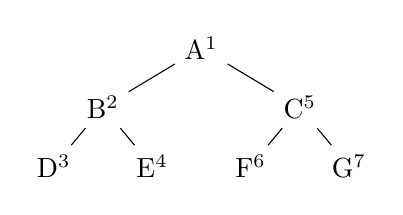
\begin{tikzpicture}[level distance=0.75cm, level/.style={sibling distance=2.5cm/#1}]
                \node {A\textsuperscript{1}}
                child {node {B\textsuperscript{2}}
                        child {node {D\textsuperscript{3}}}
                        child {node {E\textsuperscript{4}}}
                    }
                child {node {C\textsuperscript{5}}
                        child {node {F\textsuperscript{6}}}
                        child {node {G\textsuperscript{7}}}
                    };
            \end{tikzpicture}\vspace{1em}
        \end{minipage}

        \subparagraph{Post-ordre} $D, E, B, F, G, C, A$\mbox{}\\
        \begin{minipage}
            \centering
            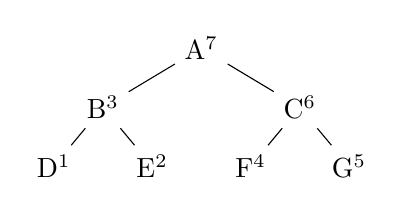
\begin{tikzpicture}[level distance=0.75cm, level/.style={sibling distance=2.5cm/#1}]
                \node {A\textsuperscript{7}}
                child {node {B\textsuperscript{3}}
                        child {node {D\textsuperscript{1}}}
                        child {node {E\textsuperscript{2}}}
                    }
                child {node {C\textsuperscript{6}}
                        child {node {F\textsuperscript{4}}}
                        child {node {G\textsuperscript{5}}}
                    };
            \end{tikzpicture}\vspace{1em}
        \end{minipage}

        \vfill\null
        \columnbreak

        \subparagraph{Largeur} $A, B, C, D, E, F, G$\mbox{}\\
        \begin{minipage}
            \centering
            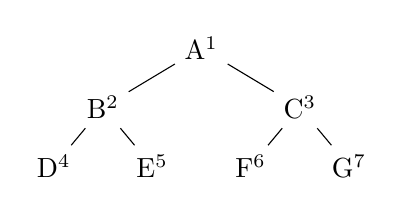
\begin{tikzpicture}[level distance=0.75cm, level/.style={sibling distance=2.5cm/#1}]
                \node {A\textsuperscript{1}}
                child {node {B\textsuperscript{2}}
                        child {node {D\textsuperscript{4}}}
                        child {node {E\textsuperscript{5}}}
                    }
                child {node {C\textsuperscript{3}}
                        child {node {F\textsuperscript{6}}}
                        child {node {G\textsuperscript{7}}}
                    };
            \end{tikzpicture}\vspace{1em}
        \end{minipage}

        \subparagraph{Symétrique (Arbres Binaires)} $D, B, E, A, F, C, G$\mbox{}\\
        \begin{minipage}
            \centering
            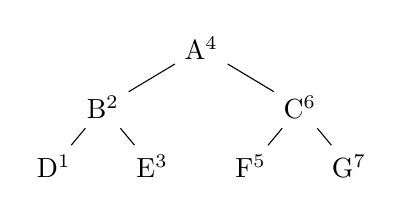
\begin{tikzpicture}[level distance=0.75cm, level/.style={sibling distance=2.5cm/#1}]
                \node {A\textsuperscript{4}}
                child {node {B\textsuperscript{2}}
                        child {node {D\textsuperscript{1}}}
                        child {node {E\textsuperscript{3}}}
                    }
                child {node {C\textsuperscript{6}}
                        child {node {F\textsuperscript{5}}}
                        child {node {G\textsuperscript{7}}}
                    };
            \end{tikzpicture}\vspace{1em}
        \end{minipage}

        \sep
        \paragraph{Arbres binaires de recherche} $n_g \leq n < n_d$, de complexité $\mathcal{O}(\log_2(n))$ si équilibré
        \subparagraph{Suppression}
        \begin{itemize}
            \item Feuille: supprimer
            \item Degré 1: remplacer par enfant
            \item Degré 2: choisir un des noeuds descendant comme racine du sous-arbre à raccrocher (1) Minimum du sous-arbre droit, (2) Maximum du sous-arbre gauche
        \end{itemize}
        \subparagraph{Taille} Nombre de noeuds dans l'arbre
        \subparagraph{Rang d'une clé} Nombre de clés plus petites que la clé donnée
        \subparagraph{Équilibre} $-1 \leq \text{hauteur}(n_g) - \text{hauteur}(n_d) \leq 1$
        % (TODO: Add STL tree data structures)

        \sep
        \paragraph{Tables de hachage}
        \subparagraph{Fonction de hachage} $h(k) = k \mod M$ avec $M$ premier et éloigné de puissances de 2
        \subparagraph{Adressage MAD} $h(k) = (a \cdot k + b) \mod M$ avec $a, b \in \mathbb{N}$ et non multiples de $M$
        % (TODO: Add more algorithms)

        \paragraph{Résolution de collisions}
        \subparagraph{Chainage} Liste chaînée à chaque case $M \approx \frac{N}{4}$ avec $M$ listes chainées et $N$ paires clé-valeur (\highlight{$M < N$})
        \begin{itemize}
            \item Doubler $M$ quand $\frac{N}{M} \geq 8$
            \item Diviser $M$ par 2 quand $\frac{N}{M} \leq 2$
        \end{itemize}
        \subparagraph{Insertion} Insertion \highlight{au début} de la liste chaînée
        \paragraph{Adressage ouvert} $M \approx 2N$ (\highlight{$M > N$})
        \subparagraph{Sondage Linéaire} Chercher la clé $k$. Si occupé, placer à la case $h(k) + i \mod M$ avec $i = 1, 2, 3, \ldots$
        \begin{itemize}
            \item Doubler $M$ quand $\frac{N}{M} \geq \frac{1}{2}$
            \item Diviser $M$ par 2 quand $\frac{N}{M} \leq \frac{1}{8}$
        \end{itemize}
        \subparagraph{Suppression} Ré-insérer les éléments suivants à la case $h(k)$

        \paragraph{Comparaisons}\mbox{}\\
        \begin{tabular}{l|c|c|c}
                             & \textbf{Insérer}                           & \textbf{Rechercher}                        & \textbf{Supprimer}                         \\
            \hline
            Tableau trié     & \cellcolor{corange!30}$\mathcal{O}(n)$     & \cellcolor{clime!30}$\mathcal{O}(\log(n))$ & \cellcolor{corange!30}$\mathcal{O}(n)$     \\
            Tableau non trié & \cellcolor{cgreen!30}$\mathcal{O}(1)$      & \cellcolor{corange!30}$\mathcal{O}(n)$     & \cellcolor{corange!30}$\mathcal{O}(n)$     \\
            Liste triée      & \cellcolor{corange!30}$\mathcal{O}(n)$     & \cellcolor{corange!30}$\mathcal{O}(n)$     & \cellcolor{corange!30}$\mathcal{O}(n)$     \\
            Liste non triée  & \cellcolor{cgreen!30}$\mathcal{O}(1)$      & \cellcolor{corange!30}$\mathcal{O}(n)$     & \cellcolor{corange!30}$\mathcal{O}(n)$     \\
            Arbre            & \cellcolor{clime!30}$\mathcal{O}(\log(n))$ & \cellcolor{clime!30}$\mathcal{O}(\log(n))$ & \cellcolor{clime!30}$\mathcal{O}(\log(n))$ \\
            Table de hachage & \cellcolor{cgreen!30}$\mathcal{O}(1)$      & \cellcolor{cgreen!30}$\mathcal{O}(1)$      & \cellcolor{cgreen!30}$\mathcal{O}(1)$      \\
        \end{tabular}\\\\
        \sep
        \paragraph{Graphes}\mbox{}\vspace*{0.25em}
        \par\textbf{Simple} Pas de boucles, pas de multi-arêtes
        \par\textbf{Degré} Nombre de sommets adjacents
        \par\textbf{Circuit} Chemin fermé

        \paragraph{Matrice d'adjacence} $M_{ij} = \deg(v_i, v_j)$
        \subparagraph{Complexité} $\mathcal{O}(n^2)$ coût mémoire, $\mathcal{O}(1)$ pour accéder à une arête, $\mathcal{O}(n)$ pour parcourir les voisins, $\mathcal{O}(n^2)$ pour parcourir tous les arêtes

        \paragraph{Liste d'adjacence} Liste des voisins
        \begin{itemize}
            \item \textbf{Non orienté} $\text{Adj}[u] = \{v \mid (u, v) \in E\}$
            \item \textbf{Orienté} $\text{Succ}[u] = \{v \mid (u, v) \in E\}$
            \item \textbf{Pondéré} $\text{Adj}[u] = \{(v, w) \mid (u, v, w) \in E\}$
        \end{itemize}
        \subparagraph{Complexité} $\mathcal{O}(n + m)$ coût mémoire, $\mathcal{O}(\deg(u))$ pour accéder à une arête, $\mathcal{O}(\deg(u))$ pour parcourir les voisins, $\mathcal{O}(n + m)$ pour parcourir tous les arêtes ($\mathcal{O}(\deg(u)) \approx \mathcal{O}(\frac{m}{n})$)

        \subparagraph{DFS (pré)} En profondeur, récursif
        \subparagraph{BFS (post)} En largeur, file FIFO
        \subparagraph{Complexité parcours} $\mathcal{O}(n^2)$ pour matrice, $\mathcal{O}(n + m)$ pour liste
        \paragraph{Tri topologique} Inverse du post-ordre d'un DAG (ne fonctionne pas sur un graphe cyclique)
        \paragraph{CC} (Composantes Connexes) Est-ce que $u$ et $v$ sont connectés?
        \paragraph{CFC} (Composantes Fortement Connexes) Est-ce que $u$ et $v$ sont connectés dans les deux sens?
        \begin{enumerate}
            \item Calculer post-ordre inverse de \highlight{l'inverse de $G$}
            \item Calculer les CFC par DFS sur $G$ dans cet ordre
        \end{enumerate}

        \vfill\null
        \columnbreak

        \section*{Usage Reference}

        \paragraph{Containers}\mbox{}
        \par\noindent\lstinline{<>.insert} Inserts an element \highlight{before} the specified position
        \par\noindent\lstinline{<>.splice} Transfers element(s) from one list to another
        \par\noindent\lstinline{<>.splice_after} Transfers element(s) \highlight{after} the specified position
        \\\sep

        \paragraph{Algorithms}\mbox{}
        \par\noindent\textcolor{clime}{\texttt{lower\_bound}} (Sorted input) Returns an iterator pointing to \highlight{first element \textbf{not} < value}. Return \texttt{end()} if no such element
        \par\noindent\textcolor{clime}{\texttt{upper\_bound}} (Sorted input) Returns an iterator pointing to \highlight{first element > value}. Return \texttt{end()} if no such element
        \par\noindent\textcolor{corange}{\texttt{nth\_element}} Rearranges the elements in the range \highlight{[first, last)} such that the element at the \texttt{nth} position is the element that would be in that position in a sorted sequence
        \\\sepdotted
        \par\noindent\textcolor{corange}{\texttt{partition}} Rearranges the elements in the range \highlight{[first, last)} such that \texttt{pred} is \True{} for elements before the partition and \False{} for elements after. Returns an iterator to the first element of the second group
        \par\noindent\textcolor{corange}{\texttt{partition\_point}} Returns an iterator to the first element in the range \highlight{[first, last)} for which \texttt{pred} is \False{}
        \\\sepdotted
        \par\noindent\textcolor{cred}{\texttt{partial\_sort}} Sort until \texttt{middle} in the range \highlight{[first, last)}
        \par\noindent\textcolor{corange}{\texttt{adjacent\_find}} Returns an iterator to the first element in the range \highlight{[first, last)} that is equal to the next element
        \\\sepdotted
        \par\noindent\textcolor{clime}{\texttt{push\_heap}} (Is already heap) \highlight{Inserts \texttt{last$-1$}} element into the correct position of the heap
        \par\noindent\textcolor{clime}{\texttt{pop\_heap}} (Is already heap) \highlight{Swaps the \texttt{first} and \texttt{last$-1$}} element and rearranges the heap
        \\\sep

        \paragraph{Iterators}\mbox{}\\
        \par\noindent\begin{minipage}
            \centering
            \begin{tabular}{|l|l|l|l||l|}
                \hline
                \multicolumn{4}{|l||}{\textbf{All}} & \makecell[l]{incrementation                                                                                                          \\copy-constructible/assignable\\destructible}                                                                                                                       \\ \hline
                \multirow{5}{*}{\texttt{RA}}        & \multirow{4}{*}{\texttt{Bi}} & \multirow{3}{*}{\texttt{Fw}}                    & \texttt{In}    & \makecell[l]{\texttt{==, !=}       \\dereferenced as an \textit{rvalue}}\\ \cline{4-5}
                                                    &                              &                                                 & \texttt{Out}   & dereferenced as an \textit{lvalue} \\ \cline{4-5}
                                                    &                              &                                                 &                & \makecell[l]{default-constructible \\multi-pass\textsuperscript{1}} \\ \cline{3-5}
                                                    &                              & \multicolumn{2}{l||}{}                          & decrementation                                      \\ \cline{2-5}
                                                    & \multicolumn{3}{l||}{}       & \texttt{+, -, +=, -=, <, >, $\leq$, $\geq$, []}                                                       \\ \hline
            \end{tabular}\vspace*{0.1em}
            \textsuperscript{1}neither dereferencing nor incrementing affects dereferenceability
        \end{minipage}
        \par\noindent\textcolor{corange}{\texttt{advance}, \texttt{distance}, \texttt{next}, \texttt{prev}} \textsc{complexity} $\mathcal{O}(1)$ for \texttt{RA}, otherwise $\mathcal{O}(n)$
\end{multicols*}

\pagebreak

\begin{multicols*}{4}
    \footnotesize

    \paragraph{Permuter les $n$ premiers caractères}
    \sep
    \begin{algorithmic}
        \Function{Permuter}{$S$, $n$} \Comment{$e = n \cdot n!$}
        \If{$n = 1$}
        \State $\Call{traiter}{S}$
        \Else
        \For{$i = 1$ to $n$}
        \State $\Call{Permuter}{S, n - 1}$
        \State $\Call{swap}{S[i], S[n]}$
        \EndFor
        \EndIf
        \EndFunction
    \end{algorithmic}
    \sepdotted
    \begin{algorithmic}
        \Function{Permuter}{$S$, $n$} \Comment{$e = 3.43 \cdot n!$}
        \If{$n = 1$}
        \State $\Call{traiter}{S}$
        \Else
        \For{$i = 1$ to $n$}
        \State $\Call{swap}{S[i], S[n]}$
        \State $\Call{Permuter}{S, n - 1}$
        \State \highlight{\Call{swap}{$S[i]$, $S[n]$}}
        \EndFor
        \EndIf
        \EndFunction
    \end{algorithmic}
    \sepdotted
    \begin{algorithmic}
        \Function{Permuter}{$S$, $n$} \Comment{$e = 2(n! - 1)$}
        \If{$n = 1$}
        \State $\Call{traiter}{S}$
        \Else
        \For{$i = 1$ to \highlight{$n-1$}}
        \State $\Call{swap}{S[i], S[n]}$
        \State $\Call{Permuter}{S, n - 1}$
        \State $\Call{swap}{S[i], S[n]}$
        \EndFor
        \State \highlight{\Call{Permuter}{$S$, $n - 1$}}
        \EndIf
        \EndFunction
    \end{algorithmic}
    \sepdotted
    \begin{algorithmic}
        \Function{Permuter}{$S$, $n$} \Comment{$e = n! - 1$}
        \If{$n = 1$}
        \State $\Call{traiter}{S}$
        \Else
        \State $\Call{Permuter}{S, n - 1}$
        \For{$i = 1$ to $n-1$}
        \If{\highlight{$n$ is even}}
        \State \highlight{\Call{swap}{$S[i]$, $S[n]}$}
        \Else
        \State \highlight{\Call{swap}{$S[1]$, $S[n]}$}
        \EndIf
        \State $\Call{Permuter}{S, n - 1}$
        \EndFor
        \EndIf
        \EndFunction
    \end{algorithmic}

    \paragraph{Tris}\mbox{}\\
    \sep
    \begin{algorithmic}
        \Function{BubbleSort}{$A$, $n$}
        \For{$i = 1$ to $n - 1$}
        \For{$j = 1$ to $n - i$}
        \If{$A[j + 1] < A[j]$}
        \State $\Call{swap}{A[j], A[j + 1]}$
        \EndIf
        \EndFor
        \EndFor
        \EndFunction
    \end{algorithmic}
    \sepdotted
    \begin{algorithmic}
        \Function{SelectionSort}{$A$, $n$}
        \For{$i = 1$ to $n-1$}
        \State $imin \gets i$
        \For{$j = i + 1$ to $n$}
        \If{$A[j] < A[imin]$}
        \State $imin \gets j$
        \EndIf
        \EndFor
        \State $\Call{swap}{A[i], A[imin]}$
        \EndFor
        \EndFunction
    \end{algorithmic}
    \sepdotted
    \begin{algorithmic}
        \Function{InsertionSort}{$A$, $n$}
        \For{$i = 2$ to $n$}
        \State $tmp \gets A[i]$
        \State $j \gets i$
        \While{$j - 1 \geq 1$ \algkw{and} $A[j - 1] > tmp$}
        \State $A[j] \gets A[j - 1]$
        \State $j \gets j - 1$
        \EndWhile
        \State $A[j] \gets tmp$
        \EndFor
        \EndFunction
    \end{algorithmic}
    \sepdotted
    \begin{algorithmic}
        \Function{Fusionner}{$A$, $p$, $q$, $r$}
        \State $L \gets$ copy of subarray $A[p \ldots q]$
        \State $R \gets$ copy of subarray $A[q + 1 \ldots r]$
        \State insert a sentinel value $\infty$ at the end of $L$ and $R$
        \State $i \gets 1$, $j \gets 1$
        \For{$k = p$ to $r$}
        \If{$L[i] \leq R[j]$}
        \State $A[k] \gets L[i]$
        \State $i \gets i + 1$
        \Else
        \State $A[k] \gets R[j]$
        \State $j \gets j + 1$
        \EndIf
        \EndFor
        \EndFunction
    \end{algorithmic}
    \columnbreak

    \begin{algorithmic}
        \Function{TriFusion}{$A$, $lo$, $hi$}
        \If{$hi \leq lo$}
        \State \Return
        \EndIf
        \State $mid \gets lo + (hi - lo)/2$\\
        \State $\Call{TriFusion}{A, lo, mid}$
        \State $\Call{TriFusion}{A, mid + 1, hi}$
        \State $\Call{Fusionner}{A, lo, mid, hi}$
        \EndFunction
    \end{algorithmic}
    \sepdotted
    \begin{algorithmic}
        \Function{Partition}{$A$, $lo$, $hi$}
        \State $i \gets lo-1$, $j \gets hi$
        \While{\True}
        \Repeat
        \State $i \gets i + 1$
        \Until{$A[i] \geq A[hi]$}
        \Repeat
        \State $j \gets j - 1$
        \Until{$j \leq lo$ \algkw{or} $A[hi] \geq A[j]$}
        \If{$i \geq j$}
        \Break
        \EndIf
        \State $\Call{swap}{A[i], A[j]}$
        \EndWhile
        \State $\Call{swap}{A[i], A[hi]}$
        \State \Return $i$
        \EndFunction
    \end{algorithmic}
    \sepdotted
    \begin{algorithmic}
        \Function{TriRapide}{$A$, $lo$, $hi$}
        \If{$lo < hi$}
        \State $p \gets$ choose pivot element
        \State $\Call{swap}{A[hi], A[p]}$
        \State $i \gets$ \Call{Partition}{$A$, $lo$, $hi$}\\
        \State $\Call{QuickSort}{A, lo, i - 1}$
        \State $\Call{QuickSort}{A, i + 1, hi}$
        \EndIf
        \EndFunction
    \end{algorithmic}
    \sepdotted
    \begin{algorithmic}
        \Function{QuickSort}{$A$, $lo$, $hi$}
        \While{$lo < hi$}
        \State $p \gets$ choose pivot element
        \State $\Call{swap}{A[hi], A[p]}$
        \State $i \gets$ \Call{Partition}{$A$, $lo$, $hi$}\\
        \If{$i - lo < hi - i$}
        \State $\Call{QuickSort}{A, lo, i - 1}$
        \State $lo \gets i + 1$
        \Else
        \State $\Call{QuickSort}{A, i + 1, hi}$
        \State $hi \gets i - 1$
        \EndIf
        \EndWhile
        \EndFunction
    \end{algorithmic}
    \begin{algorithmic}
        \Function{SelectionRapide}{$A$, $n$, $k$}
        \State $lo \gets 1$
        \State $hi \gets n$\\
        \While{$hi > lo$}
        \State $i \gets \Call{Partition}{A, lo, hi}$
        \If{$i < k$}
        \State $lo \gets i + 1$
        \ElsIf{$i > k$}
        \State $hi \gets i - 1$
        \Else \Comment{$i = k$}
        \State \Return $A[k]$
        \EndIf
        \EndWhile\\
        \State \Return $A[k]$
        \EndFunction
    \end{algorithmic}
    \sepdotted
    \begin{algorithmic}
        \Function{TriComptage}{$A$, $n$, $b$, $key$}
        \State $C \gets$ array of $b$ counters initialized to zero
        \For{each $e$ in $A$}
        \State $C[key(e)] \gets C[key(e)] + 1$
        \EndFor\\

        \State $idx \gets 1$
        \For{$i = 1$ to $b$}
        \State $tmp \gets C[i]$
        \State $C[i] \gets idx$
        \State $idx \gets idx + tmp$
        \EndFor\\

        \State $B \gets$ array of the same size as $A$
        \For{each $e$ in $A$}
        \State $B[C[key(e)]] \gets \textbf{move } e$
        \State $C[key(e)] \gets C[key(e)] + 1$
        \EndFor

        \State \Return $B$
        \EndFunction
    \end{algorithmic}
    \sepdotted
    \begin{algorithmic}
        \Function{TriParBase}{$T$, $d$}
        \For{$i = d$ to $1$}
        \State Sort $T$ with a stable sort according to
        \State the $i$-th digit
        \EndFor
        \EndFunction
    \end{algorithmic}
    \vfill\null
\end{multicols*}

\pagebreak

\begin{multicols*}{3}
    \footnotesize

    \paragraph{Tas (Heap)}\mbox{}\\
    \sep
    \begin{algorithmic}
        \Function{Parent}{$i$}
        \Return $(i - 1)/2$
        \EndFunction
    \end{algorithmic}
    \sepdotted
    \begin{algorithmic}
        \Function{E1}{$i$}
        \Return $2 \cdot i + 1$ \Comment{Enfant gauche}
        \EndFunction
    \end{algorithmic}
    \sepdotted
    \begin{algorithmic}
        \Function{E2}{$i$}
        \Return $2 \cdot i + 2$ \Comment{Enfant droit}
        \EndFunction
    \end{algorithmic}
    \sepdotted
    \begin{algorithmic}
        \Function{Remonter}{$T$, $i$}
        \While{$i > 0$ \algkw{and} $T[\Call{Parent}{i}] < T[i]$}
        \State $\Call{swap}{T[i], T[\textsc{Parent}(i)]}$
        \State $i \gets \Call{Parent}{i}$
        \EndWhile
        \EndFunction
    \end{algorithmic}
    \sepdotted
    \begin{algorithmic}
        \Function{PGE}{$T$, $i$, $k = \textsc{taille}(T)$} \Comment{Plus grand enfant}
        \If {$\Call{E2}{i} < k$ \algkw{and} $T[\textsc{E2}(i)] > T[\textsc{E1}(i)]$}
        \State \Return $\Call{E2}{i}$
        \EndIf
        \EndFunction
    \end{algorithmic}
    \sepdotted
    \begin{algorithmic}
        \Function{Descendre}{$T$, $i$, $k = \textsc{taille}(T)$}
        \While{$\Call{E1}{i} < k$ \algkw{and} $T[\Call{PGE}{T, i, k}] > T[i]$}
        \State $\Call {swap}{T[\textsc{PGE}(T, i, k)], T[i]}$
        \State $i \gets \Call{PGE}{T, i, k}$
        \EndWhile
        \EndFunction
    \end{algorithmic}
    \sepdotted
    \begin{algorithmic}
        \Function{CreerTas}{$T$} \Comment{$\mathcal{O}(n\log(n))$}
            \For{$i = 1$ to $\Call{taille}{T} - 1$}
            \State $\Call{Remonter}{T, i}$
        \EndFor
        \EndFunction
    \end{algorithmic}
    \sepdotted
    \begin{algorithmic}
        \Function{CreerTas}{$T$} \Comment{$\mathcal{O}(n)$}
        \State $p \gets \Call{Parent}{\textsc{taille}(T) - 1}$
        \For{$i = p$ to $0$}
        \State $\Call{Descendre}{T, i}$
        \EndFor
        \EndFunction
    \end{algorithmic}
    \sepdotted
    \begin{algorithmic}
        \Function{TriParTas}{$T$} \Comment{$\mathcal{O}(n\log(n))$}
            \State $N \gets \Call{taille}{T}$
            \State $\Call{CreerTas}{T}$
            \For{$k = N - 1$ to $1$}
            \State $\Call{swap}{T[k], T[0]}$
            \State $\Call{Descendre}{T, 0, k}$
        \EndFor
        \EndFunction
    \end{algorithmic}
    \columnbreak

    \paragraph{Arbres Binaires}\mbox{}\\
    \sep
    \begin{algorithmic}
        \Function{Hauteur}{$r$}
        \If{$r = \varnothing$} \Return $0$
        \Else
        \State \Return $1 + \max(\Call{Hauteur}{r.gauche}, \Call{Hauteur}{r.droit})$
        \EndIf
        \EndFunction
    \end{algorithmic}
    \sepdotted
    \begin{algorithmic}
        \Function{Equilibre}{$r$}
        \If{$r = \varnothing$} \Return $0$
        \Else
        \State \Return $\Call{Hauteur}{r.gauche} - \Call{Hauteur}{r.droit}$
        \EndIf
        \EndFunction
    \end{algorithmic}
    \sepdotted
    \begin{algorithmic}
        \Function{Lineariser}{$r$, ref $out$, ref $n$} \Comment{$n$ compteur noeuds}
        \If{$r \neq \varnothing$}
        \State $\Call{Lineariser}{r.droit, out, n}$
        \State $r.droit \gets out$, $out \gets r$, $n \gets n + 1$
        \State $\Call{Lineariser}{r.gauche, out, n}$
        \State $r.gauche \gets \varnothing $
        \EndIf
        \EndFunction
    \end{algorithmic}
    \sepdotted
    \begin{algorithmic}
        \Function{Arboriser}{ref $out$, $n$}
        \If{$n \neq 0$}
        \State $rg \gets \Call{Arboriser}{out, (n - 1)/2}$
        \State $r \gets out$, $out.gauche \gets rg$, $out \gets out.droit$
        \State $r.droit \gets \Call{Arboriser}{out, n/2}$
        \State \Return $r$
        \EndIf
        \EndFunction
    \end{algorithmic}
    \sepdotted
    \begin{algorithmic}
        \Function{Equilibrer}{$r$} \Comment{$\mathcal{O}(n)$}
        \State $out \gets \varnothing$, $n \gets 0$
        \State $\Call{Lineariser}{r, out, n}$
        \State \Return $\Call{Arboriser}{out, n}$
        \EndFunction
    \end{algorithmic}
    \sepdotted
    \begin{algorithmic}
        \Function{RotGauche}{ref $r$}
        \State $tmp \gets r.droit$
        \State $r.droit \gets tmp.gauche$
        \State $tmp.gauche \gets r$
        \State $r \gets tmp$
        \EndFunction
    \end{algorithmic}
    \sepdotted
    \begin{algorithmic}
        \Function{RotDroite}{ref $r$}
        \State $tmp \gets r.gauche$
        \State $r.gauche \gets tmp.droit$
        \State $tmp.droit \gets r$
        \State $r \gets tmp$
        \EndFunction
    \end{algorithmic}
    \columnbreak

    \begin{algorithmic}
        \Function{RetablirEquilibre}{ref $r$}
        \If{$r = \varnothing$} \Return
        \EndIf
        \If{$\Call{Equilibre}{r} < -1$}
        \If{$\Call{Equilibre}{r.droit} > 0$}
        \State $\Call{RotDroite}{r.droit}$
        \EndIf
        \State $\Call{RotGauche}{r}$
        \ElsIf{$\Call{Equilibre}{r} > 1$}
        \If{$\Call{Equilibre}{r.gauche} < 0$}
        \State $\Call{RotGauche}{r.gauche}$
        \EndIf
        \State $\Call{RotDroite}{r}$
        \Else
        \State $\Call{CalculerHauteur}{r}$ \Comment{Mettre à jour attrib. hauteur}
        \EndIf
        \EndFunction
    \end{algorithmic}
    \sepdotted
    \begin{algorithmic}
        \Function{Inserer}{ref $r$, $k$}
        \If{$r = \varnothing$}
        \State $r \gets \algkw{new } Noeud(k)$
        \ElsIf{$k = r.cle$}
        \State \Return \Comment{Déjà présent}
        \Else
        \If{$k < r.cle$}
        \State $\Call{Inserer}{r.gauche, k}$
        \Else
        \State $\Call{Inserer}{r.droit, k}$
        \EndIf
        \State $\Call{RetablirEquilibre}{r}$
        \EndIf
        \EndFunction
    \end{algorithmic}
    \sepdotted
    \begin{algorithmic}
        \Function{Supprimer}{ref $r$, $k$}
        \If{$r = \varnothing$}
        \State \Return
        \EndIf
        \If{$k = r.cle$}
        \State Suppression de $r$ avec 3 cas
        \Else
        \If{$k < r.cle$}
        \State $\Call{Supprimer}{r.gauche, k}$
        \Else
        \State $\Call{Supprimer}{r.droit, k}$
        \EndIf
        \EndIf
        \State $\Call{RetablirEquilibre}{r}$
        \EndFunction
    \end{algorithmic}
    \vfill\null
    \columnbreak

    \paragraph{Graphes}\mbox{}\\
    \sep

    \begin{algorithmic}
        \Require Les sommets sont marqués comme non visités
        \Function{Profondeur}{sommet $v$, Fn $pre$, (opt.) Fn $post$}
        \State pre($v$) \Comment{en pré-ordre}
        \State $v \gets$ visité
        \For{tout $w$ adjacent à $v$}
        \If{$w$ n'est pas visité}
        \State \Call{Profondeur}{$w$, $pre$, $post$}
        \EndIf
        \EndFor
        \State post($v$) \Comment{en post-ordre}
        \EndFunction
    \end{algorithmic}
    \sepdotted
    \begin{algorithmic}
        \Function{ProfondeurG}{Graphe $G$, Fn $action$}
        \State Marquer tous les sommets comme non visités
        \For{tout sommet $v$ de $G$}
        \If{$v$ n'est pas visité}
        \State \Call{Profondeur}{$v$, $action$}
        \EndIf
        \EndFor
        \EndFunction
    \end{algorithmic}
    \sepdotted
    \begin{algorithmic}
        \Function{Largeur}{sommet $v$, Fn $action$}
        \State Initialiser une file $Q$ vide
        \State $Q$.push($v$)
        \State $v \gets$ visité
        \While{$Q$ n'est pas vide}
        \State $v \gets$ $Q$.pop()
        \State $action$($v$)
        \For{tout $w$ adjacent à $v$}
        \If{$w$ n'est pas visité}
        \State $Q$.push($w$)
        \State $w \gets$ visité
        \EndIf
        \EndFor
        \EndWhile
        \EndFunction
    \end{algorithmic}
    \sepdotted
    \begin{algorithmic}
        \Function{ParentsEnLargeur}{sommet $v$}
        \State Initialiser un tableau $Parents$ à $-1$
        \State Initialiser une file $Q$ vide
        \State $Q$.push($v$)
        \State $Parents$[$v$] $\gets$ v \Comment{sommet d'origine}
        \While{$Q$ n'est pas vide}
        \State $v \gets$ Q.pop()
        \For{tout $w$ adjacent à $v$}
        \If{$Parents$[$w$] $ = -1$} \Comment{$w$ non marqué}
        \State $Q$.push($w$)
        \State $Parents$[$w$] $\gets v$
        \EndIf
        \EndFor
        \EndWhile
        \State \Return $Parents$
        \EndFunction
    \end{algorithmic}
    \begin{algorithmic}
        \Function{Chaine}{Parents $P$, sommet $w$}
        \State Initialiser $chaine$ vide
        \If{$P[w] = -1$}
        \State \Return $chaine$ vide
        \Else
        \While{$P[w] \neq w$}
        \State ajouter $w$ à la $chaine$
        \State $w \gets P[w]$
        \EndWhile
        \EndIf
        \State \Return $chaine$
        \EndFunction
    \end{algorithmic}
    \sepdotted
    \begin{algorithmic}
        \Function{ParentsEnLargeur}{Sommets $S$}
        \State Initialiser tableau $Parents$ à $-1$
        \State Initialiser file $Q$ vide
        \For{tout sommet $v$ de $S$}
        \State $Q$.push($v$)
        \State $Parents[v] \gets v$
        \EndFor
        \While{$Q$ n'est pas vide}
        \State $v \gets Q$.pop()
        \For{tout $w$ adjacent à $v$}
        \If{$Parents[w] = -1$}
        \State $Q$.push($w$)
        \State $Parents[w] \gets v$
        \EndIf
        \EndFor
        \EndWhile
        \State \Return $Parents$
        \EndFunction
    \end{algorithmic}
    \sepdotted
    \begin{algorithmic}
        \Function{Dijkstra}{graphe $G(V, E)$, sommet $v_0$}
        \State $Q \gets \text{PriorityQueue}()$
        \State $distTo[|V|], edgeTo[|V|]$
        \State $distTo[v_0] \gets 0$, $Q.\text{push}(v_0, 0)$\\
        \For{$v \in G$}
        \If{$v \neq v_0$}
        \State $distTo[v] \gets \infty, edgeTo[v] \gets \text{NULL}$
        \EndIf
        \EndFor
        \While {$Q$ n'est pas vide}
        \State $v \gets Q.\text{top}(), Q.\text{pop}()$
        \For{$e:v \rightarrow w \in \text{adj}(v)$}
        \State $d \gets distTo[v] + \text{weight}(e)$
        \If{$d < distTo[w]$}
        \State $distTo[w] \gets d, edgeTo[w] \gets e$
        \State $Q.\text{add\_or\_modify}(w, -distTo[w])$
        \EndIf
        \EndFor
        \EndWhile
        \State \Return $distTo[ ], edgeTo[ ]$
        \EndFunction
        \vfill\null
        \columnbreak

        \begin{algorithmic}
            \Function{ComposantesConnexes}{Graphe $G$}
            \State $id \gets 0$
            \State Initialiser tableau $CC$ à $-1$
            \For{tout sommet $v$ de $G$}
            \If{$CC[v] = -1$}
            \State \Call{Profondeur}{$v$, \algkw{fn}($v$) \{ $CC[v] \gets id$; \}}
            \State $id \gets id + 1$
            \EndIf
            \EndFor
            \State \Return $CC[ ]$
            \EndFunction
        \end{algorithmic}
        \sepdotted
        \begin{algorithmic}
            \Function{DetectionCycle}{sommet $v$}
            \State \algkw{static} $foundCycle \gets$ \False
            \State Initialiser tableau $visited$ à \True
            \State Initialiser tableau $parents$ à \True\\
            \For{tout sommet $w \in \text{adj}(v)$}
            \If{$foundCycle$}
            \State \Return
            \ElsIf{$\algkw{not } visited[w]$}
            \State \Call{DetectionCycle}{$w$}
            \ElsIf{$parents[w]$}
            \State $foundCycle \gets$ \True
            \EndIf
            \EndFor
            \State $parents[v] \gets$ \False
            \EndFunction
        \end{algorithmic}
    \end{algorithmic}
\end{multicols*}

\pagebreak

\setlength{\columnsep}{6.5pt}
\begin{multicols*}{6}
    \scriptsize
    \raggedright
    \listofmethods
    \vspace*{1.5em}
    \begin{tabular}{ll}
        \vspace{0.25em}
        \cellcolor{cgreen}  & $\mathcal{O}(1)$        \\
        \vspace{0.25em}
        \cellcolor{clime}   & $\mathcal{O}(\log(n))$  \\
        \vspace{0.25em}
        \cellcolor{corange} & $\mathcal{O}(n)$        \\
        \vspace{0.25em}
        \cellcolor{cred}    & $\mathcal{O}(n\log(n))$
    \end{tabular}

    \vfill\null
    \pagebreak
\end{multicols*}
\setlength{\columnsep}{15pt}
\begin{multicols*}{4}
    \scriptsize
    \setlength{\fboxsep}{.5\fboxsep}
\sep
\addcontentsline{mtd}{section}{1 Array}
\paragraph{1 Array}\mbox{}\vspace{0.5em}\\
\noindent\addcontentsline{mtd}{subsection}{1.01 \textcolor{cgreen}{\texttt{at}}}\boxed{1.01}\hspace*{0.25em}\lstinline[basicstyle=\ttfamily\color{cgreen}]{ref at(size_t n); const_ref at(size_t n) const;} \textsc{complexity} Constant.\\\vspace{-0.6em}

\noindent\addcontentsline{mtd}{subsection}{1.02 \textcolor{cgreen}{\texttt{back}}}\boxed{1.02}\hspace*{0.25em}\lstinline[basicstyle=\ttfamily\color{cgreen}]{ref back(); const_ref back() const;} \textsc{complexity} Constant.\\\vspace{-0.6em}

\noindent\addcontentsline{mtd}{subsection}{1.03 \textcolor{cgreen}{\texttt{begin}}}\boxed{1.03}\hspace*{0.25em}\lstinline[basicstyle=\ttfamily\color{cgreen}]{iter begin() noexcept; const_iter begin() const noexcept;} \textsc{complexity} Constant.\\\vspace{-0.6em}

\noindent\addcontentsline{mtd}{subsection}{1.04 \textcolor{cgreen}{\texttt{cbegin}}}\boxed{1.04}\hspace*{0.25em}\lstinline[basicstyle=\ttfamily\color{cgreen}]{const_iter cbegin() const noexcept;} \textsc{complexity} Constant.\\\vspace{-0.6em}

\noindent\addcontentsline{mtd}{subsection}{1.05 \textcolor{cgreen}{\texttt{cend}}}\boxed{1.05}\hspace*{0.25em}\lstinline[basicstyle=\ttfamily\color{cgreen}]{const_iter cend() const noexcept;} \textsc{complexity} Constant.\\\vspace{-0.6em}

\noindent\addcontentsline{mtd}{subsection}{1.06 \textcolor{cgreen}{\texttt{crbegin}}}\boxed{1.06}\hspace*{0.25em}\lstinline[basicstyle=\ttfamily\color{cgreen}]{const_reverse_iter crbegin() const noexcept;} \textsc{complexity} Constant.\\\vspace{-0.6em}

\noindent\addcontentsline{mtd}{subsection}{1.07 \textcolor{cgreen}{\texttt{crend}}}\boxed{1.07}\hspace*{0.25em}\lstinline[basicstyle=\ttfamily\color{cgreen}]{const_reverse_iter crend() const noexcept;} \textsc{complexity} Constant.\\\vspace{-0.6em}

\noindent\addcontentsline{mtd}{subsection}{1.08 \textcolor{cgreen}{\texttt{data}}}\boxed{1.08}\hspace*{0.25em}\lstinline[basicstyle=\ttfamily\color{cgreen}]{value_t* data() noexcept; const value_t* data() const noexcept;} \textsc{complexity} Constant.\\\vspace{-0.6em}

\noindent\addcontentsline{mtd}{subsection}{1.09 \textcolor{cgreen}{\texttt{empty}}}\boxed{1.09}\hspace*{0.25em}\lstinline[basicstyle=\ttfamily\color{cgreen}]{constexpr bool empty() noexcept;} \textsc{complexity} Constant.\\\vspace{-0.6em}

\noindent\addcontentsline{mtd}{subsection}{1.10 \textcolor{cgreen}{\texttt{end}}}\boxed{1.10}\hspace*{0.25em}\lstinline[basicstyle=\ttfamily\color{cgreen}]{iter end() noexcept; const_iter end() const noexcept;} \textsc{complexity} Constant.\\\vspace{-0.6em}

\noindent\addcontentsline{mtd}{subsection}{1.11 \textcolor{corange}{\texttt{fill}}}\boxed{1.11}\hspace*{0.25em}\lstinline[basicstyle=\ttfamily\color{corange}]{void fill(const value_t& val);} \textsc{complexity} Linear: Performs as many assignment operations as the size of the array object.\\\vspace{-0.6em}

\noindent\addcontentsline{mtd}{subsection}{1.12 \textcolor{cgreen}{\texttt{front}}}\boxed{1.12}\hspace*{0.25em}\lstinline[basicstyle=\ttfamily\color{cgreen}]{ref front(); const_ref front() const;} \textsc{complexity} Constant.\\\vspace{-0.6em}

\noindent\addcontentsline{mtd}{subsection}{1.13 \textcolor{cgreen}{\texttt{max\_size}}}\boxed{1.13}\hspace*{0.25em}\lstinline[basicstyle=\ttfamily\color{cgreen}]{constexpr size_t max_size() noexcept;} \textsc{complexity} Constant.\\\vspace{-0.6em}

\noindent\addcontentsline{mtd}{subsection}{1.14 \textcolor{cgreen}{\texttt{operator[]}}}\boxed{1.14}\hspace*{0.25em}\lstinline[basicstyle=\ttfamily\color{cgreen}]{ref operator[](size_t n); const_ref operator[](size_t n) const;} \textsc{complexity} Constant.\\\vspace{-0.6em}

\noindent\addcontentsline{mtd}{subsection}{1.15 \textcolor{cgreen}{\texttt{rbegin}}}\boxed{1.15}\hspace*{0.25em}\lstinline[basicstyle=\ttfamily\color{cgreen}]{reverse_iter rbegin() noexcept; const_reverse_iter rbegin() const noexcept;} \textsc{complexity} Constant.\\\vspace{-0.6em}

\noindent\addcontentsline{mtd}{subsection}{1.16 \textcolor{cgreen}{\texttt{rend}}}\boxed{1.16}\hspace*{0.25em}\lstinline[basicstyle=\ttfamily\color{cgreen}]{reverse_iter rend() noexcept; const_reverse_iter rend() const noexcept;} \textsc{complexity} Constant.\\\vspace{-0.6em}

\noindent\addcontentsline{mtd}{subsection}{1.17 \textcolor{cgreen}{\texttt{size}}}\boxed{1.17}\hspace*{0.25em}\lstinline[basicstyle=\ttfamily\color{cgreen}]{constexpr size_t size() noexcept;} \textsc{complexity} Constant.\\\vspace{-0.6em}

\noindent\addcontentsline{mtd}{subsection}{1.18 \textcolor{corange}{\texttt{swap}}}\boxed{1.18}\hspace*{0.25em}\lstinline[basicstyle=\ttfamily\color{corange}]{void swap(array& x) noexcept(noexcept(swap(declval<value_t&>(),declval<value_t&>())));} \textsc{complexity} Linear: Performs as many individual swap operations as the size of the arrays. \textsc{validity} The validity of all iterators, references and pointers is not changed: They remain associated with the same positions in the same container they were associated before the call, but the elements they still refer to have the swapped values.\\\vspace{-0.6em}


\sep
\addcontentsline{mtd}{section}{2 Vector}
\paragraph{2 Vector}\mbox{}\vspace{0.5em}\\
\noindent\addcontentsline{mtd}{subsection}{2.01 \textcolor{corange}{\texttt{assign}}}\boxed{2.01}\hspace*{0.25em}\lstinline[basicstyle=\ttfamily\color{corange}]{void assign(init_list<value_t> il);} \textsc{complexity} Linear on initial and final sizes (destructions, constructions).Additionally, in the range version (1), if InputIterator is not at least of a forward iterator category (i.e., it is just an input iterator) the new capacity cannot be determined beforehand and the operation incurs in additional logarithmic complexity in the new size (reallocations while growing). \textsc{validity} All iterators, pointers and references related to this container are invalidated.\\\vspace{-0.6em}

\noindent\addcontentsline{mtd}{subsection}{2.02 \textcolor{cgreen}{\texttt{at}}}\boxed{2.02}\hspace*{0.25em}\lstinline[basicstyle=\ttfamily\color{cgreen}]{ref at(size_t n); const_ref at(size_t n) const;} \textsc{complexity} Constant.\\\vspace{-0.6em}

\noindent\addcontentsline{mtd}{subsection}{2.03 \textcolor{cgreen}{\texttt{back}}}\boxed{2.03}\hspace*{0.25em}\lstinline[basicstyle=\ttfamily\color{cgreen}]{ref back(); const_ref back() const;} \textsc{complexity} Constant.\\\vspace{-0.6em}

\noindent\addcontentsline{mtd}{subsection}{2.04 \textcolor{cgreen}{\texttt{begin}}}\boxed{2.04}\hspace*{0.25em}\lstinline[basicstyle=\ttfamily\color{cgreen}]{iter begin() noexcept; const_iter begin() const noexcept;} \textsc{complexity} Constant.\\\vspace{-0.6em}

\noindent\addcontentsline{mtd}{subsection}{2.05 \textcolor{cgreen}{\texttt{capacity}}}\boxed{2.05}\hspace*{0.25em}\lstinline[basicstyle=\ttfamily\color{cgreen}]{size_t capacity() const noexcept;} \textsc{complexity} Constant.\\\vspace{-0.6em}

\noindent\addcontentsline{mtd}{subsection}{2.06 \textcolor{cgreen}{\texttt{cbegin}}}\boxed{2.06}\hspace*{0.25em}\lstinline[basicstyle=\ttfamily\color{cgreen}]{const_iter cbegin() const noexcept;} \textsc{complexity} Constant.\\\vspace{-0.6em}

\noindent\addcontentsline{mtd}{subsection}{2.07 \textcolor{cgreen}{\texttt{cend}}}\boxed{2.07}\hspace*{0.25em}\lstinline[basicstyle=\ttfamily\color{cgreen}]{const_iter cend() const noexcept;} \textsc{complexity} Constant.\\\vspace{-0.6em}

\noindent\addcontentsline{mtd}{subsection}{2.08 \textcolor{corange}{\texttt{clear}}}\boxed{2.08}\hspace*{0.25em}\lstinline[basicstyle=\ttfamily\color{corange}]{void clear() noexcept;} \textsc{complexity} Linear in size (destructions).This may be optimized to constant complexity for trivially-destructible types (such as scalar or PODs), where elements need not be destroyed. \textsc{validity} All iterators, pointers and references related to this container are invalidated.\\\vspace{-0.6em}

\noindent\addcontentsline{mtd}{subsection}{2.09 \textcolor{cgreen}{\texttt{crbegin}}}\boxed{2.09}\hspace*{0.25em}\lstinline[basicstyle=\ttfamily\color{cgreen}]{const_reverse_iter crbegin() const noexcept;} \textsc{complexity} Constant.\\\vspace{-0.6em}

\noindent\addcontentsline{mtd}{subsection}{2.10 \textcolor{cgreen}{\texttt{crend}}}\boxed{2.10}\hspace*{0.25em}\lstinline[basicstyle=\ttfamily\color{cgreen}]{const_reverse_iter crend() const noexcept;} \textsc{complexity} Constant.\\\vspace{-0.6em}

\noindent\addcontentsline{mtd}{subsection}{2.11 \textcolor{cgreen}{\texttt{data}}}\boxed{2.11}\hspace*{0.25em}\lstinline[basicstyle=\ttfamily\color{cgreen}]{value_t* data() noexcept; const value_t* data() const noexcept;} \textsc{complexity} Constant.\\\vspace{-0.6em}

\noindent\addcontentsline{mtd}{subsection}{2.12 \textcolor{corange}{\texttt{emplace}}}\boxed{2.12}\hspace*{0.25em}\lstinline[basicstyle=\ttfamily\color{corange}]{template <class... Args>iter emplace(const_iter pos, Args&&... args);} \textsc{complexity} Linear on the number of elements after position (moving).If a reallocation happens, the reallocation is itself up to linear in the entire size. \textsc{validity} If a reallocation happens, all iterators, pointers and references related to this container are invalidated.Otherwise, only those pointing to position and beyond are invalidated, with all iterators, pointers and references to elements before position guaranteed to keep referring to the same elements they were referring to before the call.\\\vspace{-0.6em}

\noindent\addcontentsline{mtd}{subsection}{2.13 \textcolor{corange}{\texttt{emplace\_back}}}\boxed{2.13}\hspace*{0.25em}\lstinline[basicstyle=\ttfamily\color{corange}]{template <class... Args> void emplace_back(Args&&... args);} \textsc{complexity} Constant (amortized time, reallocation may happen).If a reallocation happens, the reallocation is itself up to linear in the entire size. \textsc{validity} If a reallocation happens, all iterators, pointers and references related to this container are invalidated.Otherwise, only the end iterator is invalidated, and all other iterators, pointers and references to elements are guaranteed to keep referring to the same elements they were referring to before the call.\\\vspace{-0.6em}

\noindent\addcontentsline{mtd}{subsection}{2.14 \textcolor{cgreen}{\texttt{empty}}}\boxed{2.14}\hspace*{0.25em}\lstinline[basicstyle=\ttfamily\color{cgreen}]{bool empty() const noexcept;} \textsc{complexity} Constant.\\\vspace{-0.6em}

\noindent\addcontentsline{mtd}{subsection}{2.15 \textcolor{cgreen}{\texttt{end}}}\boxed{2.15}\hspace*{0.25em}\lstinline[basicstyle=\ttfamily\color{cgreen}]{iter end() noexcept; const_iter end() const noexcept;} \textsc{complexity} Constant.\\\vspace{-0.6em}

\noindent\addcontentsline{mtd}{subsection}{2.16 \textcolor{corange}{\texttt{erase}}}\boxed{2.16}\hspace*{0.25em}\lstinline[basicstyle=\ttfamily\color{corange}]{iter erase(const_iter pos); iter erase(const_iter first, const_iter last);} \textsc{complexity} Linear on the number of elements erased (destructions) plus the number of elements after the last element deleted (moving). \textsc{validity} Iterators, pointers and references pointing to position (or first) and beyond are invalidated, with all iterators, pointers and references to elements before position (or first) are guaranteed to keep referring to the same elements they were referring to before the call.\\\vspace{-0.6em}

\noindent\addcontentsline{mtd}{subsection}{2.17 \textcolor{cgreen}{\texttt{front}}}\boxed{2.17}\hspace*{0.25em}\lstinline[basicstyle=\ttfamily\color{cgreen}]{ref front(); const_ref front() const;} \textsc{complexity} Constant.\\\vspace{-0.6em}

\noindent\addcontentsline{mtd}{subsection}{2.18 \textcolor{cgreen}{\texttt{get\_allocator}}}\boxed{2.18}\hspace*{0.25em}\lstinline[basicstyle=\ttfamily\color{cgreen}]{allocator_t get_allocator() const noexcept;} \textsc{complexity} Constant.\\\vspace{-0.6em}

\noindent\addcontentsline{mtd}{subsection}{2.19 \textcolor{corange}{\texttt{insert}}}\boxed{2.19}\hspace*{0.25em}\lstinline[basicstyle=\ttfamily\color{corange}]{iter insert(const_iter pos, init_list<value_t> il);} \textsc{complexity} Linear on the number of elements inserted (copy/move construction) plus the number of elements after position (moving).Additionally, if InputIterator in the range insert (3) is not at least of a forward iterator category (i.e., just an input iterator) the new capacity cannot be determined beforehand and the insertion incurs in additional logarithmic complexity in size (reallocations).If a reallocation happens, the reallocation is itself up to linear in the entire size at the moment of the reallocation. \textsc{validity} If a reallocation happens, all iterators, pointers and references related to the container are invalidated.Otherwise, only those pointing to position and beyond are invalidated, with all iterators, pointers and references to elements before position guaranteed to keep referring to the same elements they were referring to before the call.\\\vspace{-0.6em}

\noindent\addcontentsline{mtd}{subsection}{2.20 \textcolor{cgreen}{\texttt{max\_size}}}\boxed{2.20}\hspace*{0.25em}\lstinline[basicstyle=\ttfamily\color{cgreen}]{size_t max_size() const noexcept;} \textsc{complexity} Constant.\\\vspace{-0.6em}

\noindent\addcontentsline{mtd}{subsection}{2.21 \textcolor{cgreen}{\texttt{operator[]}}}\boxed{2.21}\hspace*{0.25em}\lstinline[basicstyle=\ttfamily\color{cgreen}]{ref operator[](size_t n); const_ref operator[](size_t n) const;} \textsc{complexity} Constant.\\\vspace{-0.6em}

\noindent\addcontentsline{mtd}{subsection}{2.22 \textcolor{corange}{\texttt{operator=}}}\boxed{2.22}\hspace*{0.25em}\lstinline[basicstyle=\ttfamily\color{corange}]{vector& operator=(init_list<value_t> il);} \textsc{complexity} Linear in size. \textsc{validity} All iterators, references and pointers related to this container before the call are invalidated.In the move assignment, iterators, pointers and references referring to elements in x are also invalidated.\\\vspace{-0.6em}

\noindent\addcontentsline{mtd}{subsection}{2.23 \textcolor{cgreen}{\texttt{pop\_back}}}\boxed{2.23}\hspace*{0.25em}\lstinline[basicstyle=\ttfamily\color{cgreen}]{void pop_back();} \textsc{complexity} Constant. \textsc{validity} The end iterator and any iterator, pointer and reference referring to the removed element are invalidated.Iterators, pointers and references referring to other elements that have not been removed are guaranteed to keep referring to the same elements they were referring to before the call.\\\vspace{-0.6em}

\noindent\addcontentsline{mtd}{subsection}{2.24 \textcolor{corange}{\texttt{push\_back}}}\boxed{2.24}\hspace*{0.25em}\lstinline[basicstyle=\ttfamily\color{corange}]{void push_back(const value_t& val); void push_back(value_t&& val);} \textsc{complexity} Constant (amortized time, reallocation may happen).If a reallocation happens, the reallocation is itself up to linear in the entire size. \textsc{validity} If a reallocation happens, all iterators, pointers and references related to the container are invalidated.Otherwise, only the end iterator is invalidated, and all iterators, pointers and references to elements are guaranteed to keep referring to the same elements they were referring to before the call.\\\vspace{-0.6em}

\noindent\addcontentsline{mtd}{subsection}{2.25 \textcolor{cgreen}{\texttt{rbegin}}}\boxed{2.25}\hspace*{0.25em}\lstinline[basicstyle=\ttfamily\color{cgreen}]{reverse_iter rbegin() noexcept; const_reverse_iter rbegin() const noexcept;} \textsc{complexity} Constant.\\\vspace{-0.6em}

\noindent\addcontentsline{mtd}{subsection}{2.26 \textcolor{cgreen}{\texttt{rend}}}\boxed{2.26}\hspace*{0.25em}\lstinline[basicstyle=\ttfamily\color{cgreen}]{reverse_iter rend() noexcept; const_reverse_iter rend() const noexcept;} \textsc{complexity} Constant.\\\vspace{-0.6em}

\noindent\addcontentsline{mtd}{subsection}{2.27 \textcolor{corange}{\texttt{reserve}}}\boxed{2.27}\hspace*{0.25em}\lstinline[basicstyle=\ttfamily\color{corange}]{void reserve(size_t n);} \textsc{complexity} If a reallocation happens, linear in vector size at most. \textsc{validity} If a reallocation happens, all iterators, pointers and references related to the container are invalidated.Otherwise, they all keep referring to the same elements they were referring to before the call.\\\vspace{-0.6em}

\noindent\addcontentsline{mtd}{subsection}{2.28 \textcolor{corange}{\texttt{resize}}}\boxed{2.28}\hspace*{0.25em}\lstinline[basicstyle=\ttfamily\color{corange}]{void resize(size_t n); void resize(size_t n, const value_t& val);} \textsc{complexity} Linear on the number of elements inserted/erased (constructions/destructions).If a reallocation happens, the reallocation is itself up to linear in the entire vector size. \textsc{validity} In case the container shrinks, all iterators, pointers and references to elements that have not been removed remain valid after the resize and refer to the same elements they were referring to before the call.If the container expands, the end iterator is invalidated and, if it has to reallocate storage, all iterators, pointers and references related to this container are also invalidated.\\\vspace{-0.6em}

\noindent\addcontentsline{mtd}{subsection}{2.29 \textcolor{corange}{\texttt{shrink\_to\_fit}}}\boxed{2.29}\hspace*{0.25em}\lstinline[basicstyle=\ttfamily\color{corange}]{void shrink_to_fit();} \textsc{complexity} At most, linear in container size. \textsc{validity} If a reallocation happens, all iterators, pointers and references related to the container are invalidated.Otherwise, no changes.\\\vspace{-0.6em}

\noindent\addcontentsline{mtd}{subsection}{2.30 \textcolor{cgreen}{\texttt{size}}}\boxed{2.30}\hspace*{0.25em}\lstinline[basicstyle=\ttfamily\color{cgreen}]{size_t size() const noexcept;} \textsc{complexity} Constant.\\\vspace{-0.6em}

\noindent\addcontentsline{mtd}{subsection}{2.31 \textcolor{cgreen}{\texttt{swap}}}\boxed{2.31}\hspace*{0.25em}\lstinline[basicstyle=\ttfamily\color{cgreen}]{void swap(vector& x);} \textsc{complexity} Constant. \textsc{validity} All iterators, pointers and references referring to elements in both containers remain valid, and are now referring to the same elements they referred to before the call, but in the other container, where they now iterate.Note that the end iterators do not refer to elements and may be invalidated.\\\vspace{-0.6em}


\sep
\addcontentsline{mtd}{section}{3 List}
\paragraph{3 List}\mbox{}\vspace{0.5em}\\
\noindent\addcontentsline{mtd}{subsection}{3.01 \textcolor{corange}{\texttt{assign}}}\boxed{3.01}\hspace*{0.25em}\lstinline[basicstyle=\ttfamily\color{corange}]{void assign(init_list<value_t> il);} \textsc{complexity} Linear in initial and final sizes (destructions, constructions). \textsc{validity} All iterators, references and pointers related to this container are invalidated, except the end iterators.\\\vspace{-0.6em}

\noindent\addcontentsline{mtd}{subsection}{3.02 \textcolor{cgreen}{\texttt{back}}}\boxed{3.02}\hspace*{0.25em}\lstinline[basicstyle=\ttfamily\color{cgreen}]{ref back(); const_ref back() const;} \textsc{complexity} Constant.\\\vspace{-0.6em}

\noindent\addcontentsline{mtd}{subsection}{3.03 \textcolor{cgreen}{\texttt{begin}}}\boxed{3.03}\hspace*{0.25em}\lstinline[basicstyle=\ttfamily\color{cgreen}]{iter begin() noexcept; const_iter begin() const noexcept;} \textsc{complexity} Constant.\\\vspace{-0.6em}

\noindent\addcontentsline{mtd}{subsection}{3.04 \textcolor{cgreen}{\texttt{cbegin}}}\boxed{3.04}\hspace*{0.25em}\lstinline[basicstyle=\ttfamily\color{cgreen}]{const_iter cbegin() const noexcept;} \textsc{complexity} Constant.\\\vspace{-0.6em}

\noindent\addcontentsline{mtd}{subsection}{3.05 \textcolor{cgreen}{\texttt{cend}}}\boxed{3.05}\hspace*{0.25em}\lstinline[basicstyle=\ttfamily\color{cgreen}]{const_iter cend() const noexcept;} \textsc{complexity} Constant.\\\vspace{-0.6em}

\noindent\addcontentsline{mtd}{subsection}{3.06 \textcolor{corange}{\texttt{clear}}}\boxed{3.06}\hspace*{0.25em}\lstinline[basicstyle=\ttfamily\color{corange}]{void clear() noexcept;} \textsc{complexity} Linear in list::size (destructions). \textsc{validity} All iterators, references and pointers related to this container are invalidated, except the end iterators.\\\vspace{-0.6em}

\noindent\addcontentsline{mtd}{subsection}{3.07 \textcolor{cgreen}{\texttt{crbegin}}}\boxed{3.07}\hspace*{0.25em}\lstinline[basicstyle=\ttfamily\color{cgreen}]{const_reverse_iter crbegin() const noexcept;} \textsc{complexity} Constant.\\\vspace{-0.6em}

\noindent\addcontentsline{mtd}{subsection}{3.08 \textcolor{cgreen}{\texttt{crend}}}\boxed{3.08}\hspace*{0.25em}\lstinline[basicstyle=\ttfamily\color{cgreen}]{const_reverse_iter crend() const noexcept;} \textsc{complexity} Constant.\\\vspace{-0.6em}

\noindent\addcontentsline{mtd}{subsection}{3.09 \textcolor{cgreen}{\texttt{emplace}}}\boxed{3.09}\hspace*{0.25em}\lstinline[basicstyle=\ttfamily\color{cgreen}]{template <class... Args> iter emplace(const_iter pos, Args&&... args);} \textsc{complexity} Constant.\\\vspace{-0.6em}

\noindent\addcontentsline{mtd}{subsection}{3.10 \textcolor{cgreen}{\texttt{emplace\_back}}}\boxed{3.10}\hspace*{0.25em}\lstinline[basicstyle=\ttfamily\color{cgreen}]{template <class... Args> void emplace_back(Args&&... args);} \textsc{complexity} Constant.\\\vspace{-0.6em}

\noindent\addcontentsline{mtd}{subsection}{3.11 \textcolor{cgreen}{\texttt{emplace\_front}}}\boxed{3.11}\hspace*{0.25em}\lstinline[basicstyle=\ttfamily\color{cgreen}]{template <class... Args> void emplace_front(Args&&... args);} \textsc{complexity} Constant. \textsc{validity} No changes.Member begin returns a different iterator value.\\\vspace{-0.6em}

\noindent\addcontentsline{mtd}{subsection}{3.12 \textcolor{cgreen}{\texttt{empty}}}\boxed{3.12}\hspace*{0.25em}\lstinline[basicstyle=\ttfamily\color{cgreen}]{bool empty() const noexcept;} \textsc{complexity} Constant.\\\vspace{-0.6em}

\noindent\addcontentsline{mtd}{subsection}{3.13 \textcolor{cgreen}{\texttt{end}}}\boxed{3.13}\hspace*{0.25em}\lstinline[basicstyle=\ttfamily\color{cgreen}]{iter end() noexcept; const_iter end() const noexcept;} \textsc{complexity} Constant.\\\vspace{-0.6em}

\noindent\addcontentsline{mtd}{subsection}{3.14 \textcolor{corange}{\texttt{erase}}}\boxed{3.14}\hspace*{0.25em}\lstinline[basicstyle=\ttfamily\color{corange}]{iter erase(const_iter pos); iter erase(const_iter first, const_iter last);} \textsc{complexity} Linear in the number of elements erased (destructions). \textsc{validity} Iterators, pointers and references referring to elements removed by the function are invalidated.All other iterators, pointers and references keep their validity.\\\vspace{-0.6em}

\noindent\addcontentsline{mtd}{subsection}{3.15 \textcolor{cgreen}{\texttt{front}}}\boxed{3.15}\hspace*{0.25em}\lstinline[basicstyle=\ttfamily\color{cgreen}]{ref front(); const_ref front() const;} \textsc{complexity} Constant.\\\vspace{-0.6em}

\noindent\addcontentsline{mtd}{subsection}{3.16 \textcolor{cgreen}{\texttt{get\_allocator}}}\boxed{3.16}\hspace*{0.25em}\lstinline[basicstyle=\ttfamily\color{cgreen}]{allocator_t get_allocator() const noexcept;} \textsc{complexity} Constant.\\\vspace{-0.6em}

\noindent\addcontentsline{mtd}{subsection}{3.17 \textcolor{corange}{\texttt{insert}}}\boxed{3.17}\hspace*{0.25em}\lstinline[basicstyle=\ttfamily\color{corange}]{iter insert(const_iter pos, init_list<value_t> il);} \textsc{complexity} Linear in the number of elements inserted (copy/move construction).\\\vspace{-0.6em}

\noindent\addcontentsline{mtd}{subsection}{3.18 \textcolor{corange}{\texttt{max\_size}}}\boxed{3.18}\hspace*{0.25em}\lstinline[basicstyle=\ttfamily\color{corange}]{size_t max_size() const noexcept;} \textsc{complexity} Up to linear.Constant.\\\vspace{-0.6em}

\noindent\addcontentsline{mtd}{subsection}{3.19 \textcolor{corange}{\texttt{merge}}}\boxed{3.19}\hspace*{0.25em}\lstinline[basicstyle=\ttfamily\color{corange}]{template <class Compare> void merge(list& x, Compare comp); template <class Compare> void merge(list&& x, Compare comp);} \textsc{complexity} At most, linear in the sum of both container sizes minus one (comparisons). \textsc{validity} No changes on the iterators, pointers and references related to the container before the call.The iterators, pointers and references that referred to transferred elements keep referring to those same elements, but iterators now iterate into the container the elements have been transferred to.\\\vspace{-0.6em}

\noindent\addcontentsline{mtd}{subsection}{3.20 \textcolor{corange}{\texttt{operator=}}}\boxed{3.20}\hspace*{0.25em}\lstinline[basicstyle=\ttfamily\color{corange}]{list& operator=(init_list<value_t> il);} \textsc{complexity} Linear in size. \textsc{validity} All iterators, references and pointers related to this container are invalidated, except the end iterators.In the move assignment, iterators, pointers and references referring to elements in x are also invalidated.\\\vspace{-0.6em}

\noindent\addcontentsline{mtd}{subsection}{3.21 \textcolor{cgreen}{\texttt{pop\_back}}}\boxed{3.21}\hspace*{0.25em}\lstinline[basicstyle=\ttfamily\color{cgreen}]{void pop_back();} \textsc{complexity} Constant. \textsc{validity} Iterators, pointers and references referring to element removed by the function are invalidated.All other iterators, pointers and reference keep their validity.\\\vspace{-0.6em}

\noindent\addcontentsline{mtd}{subsection}{3.22 \textcolor{cgreen}{\texttt{pop\_front}}}\boxed{3.22}\hspace*{0.25em}\lstinline[basicstyle=\ttfamily\color{cgreen}]{void pop_front();} \textsc{complexity} Constant. \textsc{validity} Iterators, pointers and references referring to the element removed by the function are invalidated.All other iterators, pointers and reference keep their validity.\\\vspace{-0.6em}

\noindent\addcontentsline{mtd}{subsection}{3.23 \textcolor{cgreen}{\texttt{push\_back}}}\boxed{3.23}\hspace*{0.25em}\lstinline[basicstyle=\ttfamily\color{cgreen}]{void push_back(const value_t& val); void push_back(value_t&& val);} \textsc{complexity} Constant.\\\vspace{-0.6em}

\noindent\addcontentsline{mtd}{subsection}{3.24 \textcolor{cgreen}{\texttt{push\_front}}}\boxed{3.24}\hspace*{0.25em}\lstinline[basicstyle=\ttfamily\color{cgreen}]{void push_front(const value_t& val); void push_front(value_t&& val);} \textsc{complexity} Constant.\\\vspace{-0.6em}

\noindent\addcontentsline{mtd}{subsection}{3.25 \textcolor{cgreen}{\texttt{rbegin}}}\boxed{3.25}\hspace*{0.25em}\lstinline[basicstyle=\ttfamily\color{cgreen}]{reverse_iter rbegin() noexcept; const_reverse_iter rbegin() const noexcept;} \textsc{complexity} Constant.\\\vspace{-0.6em}

\noindent\addcontentsline{mtd}{subsection}{3.26 \textcolor{corange}{\texttt{remove}}}\boxed{3.26}\hspace*{0.25em}\lstinline[basicstyle=\ttfamily\color{corange}]{void remove(const value_t& val);} \textsc{complexity} Linear in container size (comparisons). \textsc{validity} Iterators, pointers and references referring to elements removed by the function are invalidated.All other iterators, pointers and reference keep their validity.\\\vspace{-0.6em}

\noindent\addcontentsline{mtd}{subsection}{3.27 \textcolor{corange}{\texttt{remove\_if}}}\boxed{3.27}\hspace*{0.25em}\lstinline[basicstyle=\ttfamily\color{corange}]{template <class Pred> void remove_if(Pred pred);} \textsc{complexity} Linear in list size (applications of pred). \textsc{validity} Iterators, pointers and references referring to elements removed by the function are invalidated.All other iterators, pointers and reference keep their validity.\\\vspace{-0.6em}

\noindent\addcontentsline{mtd}{subsection}{3.28 \textcolor{cgreen}{\texttt{rend}}}\boxed{3.28}\hspace*{0.25em}\lstinline[basicstyle=\ttfamily\color{cgreen}]{reverse_iter rend() nothrow; const_reverse_iter rend() const nothrow;} \textsc{complexity} Constant.\\\vspace{-0.6em}

\noindent\addcontentsline{mtd}{subsection}{3.29 \textcolor{corange}{\texttt{resize}}}\boxed{3.29}\hspace*{0.25em}\lstinline[basicstyle=\ttfamily\color{corange}]{void resize(size_t n); void resize(size_t n, const value_t& val);} \textsc{complexity} If the container grows, linear in the number number of elements inserted (constructor).If the container shrinks, linear in the number of elements erased (destructions), plus up to linear in the size (iterator advance). \textsc{validity} Iterators, pointers and references referring to elements removed by the function are invalidated.All other iterators, pointers and references keep their validity.\\\vspace{-0.6em}

\noindent\addcontentsline{mtd}{subsection}{3.30 \textcolor{corange}{\texttt{reverse}}}\boxed{3.30}\hspace*{0.25em}\lstinline[basicstyle=\ttfamily\color{corange}]{void reverse() noexcept;} \textsc{complexity} Linear in list size.\\\vspace{-0.6em}

\noindent\addcontentsline{mtd}{subsection}{3.31 \textcolor{corange}{\texttt{size}}}\boxed{3.31}\hspace*{0.25em}\lstinline[basicstyle=\ttfamily\color{corange}]{size_t size() const noexcept;} \textsc{complexity} Up to linear.Constant.\\\vspace{-0.6em}

\noindent\addcontentsline{mtd}{subsection}{3.32 \textcolor{cred}{\texttt{sort}}}\boxed{3.32}\hspace*{0.25em}\lstinline[basicstyle=\ttfamily\color{cred}]{template <class Compare> void sort(Compare comp);} \textsc{complexity} Approximately NlogN where N is the container size.\\\vspace{-0.6em}

\noindent\addcontentsline{mtd}{subsection}{3.33 \textcolor{corange}{\texttt{splice}}}\boxed{3.33}\hspace*{0.25em}\lstinline[basicstyle=\ttfamily\color{corange}]{void splice(const_iter pos, list& x, const_iter first, const_iter last); void splice(const_iter pos, list&& x, const_iter first, const_iter last);} \textsc{complexity} Constant for (1) and (2).Up to linear in the number of elements transferred for (3). \textsc{validity} No changes on the iterators, pointers and references related to the container before the call.The iterators, pointers and references that referred to transferred elements keep referring to those same elements, but iterators now iterate into the container the elements have been transferred to.\\\vspace{-0.6em}

\noindent\addcontentsline{mtd}{subsection}{3.34 \textcolor{cgreen}{\texttt{swap}}}\boxed{3.34}\hspace*{0.25em}\lstinline[basicstyle=\ttfamily\color{cgreen}]{void swap(list& x);} \textsc{complexity} Constant. \textsc{validity} All iterators, pointers and references referring to elements in both containers remain valid, but now are referring to elements in the other container, and iterate in it.Note that the end iterators do not refer to elements and may be invalidated.\\\vspace{-0.6em}

\noindent\addcontentsline{mtd}{subsection}{3.35 \textcolor{corange}{\texttt{unique}}}\boxed{3.35}\hspace*{0.25em}\lstinline[basicstyle=\ttfamily\color{corange}]{template <class BinaryPred> void unique(BinaryPred binary_pred);} \textsc{complexity} Linear in container size minus one. \textsc{validity} Iterators, pointers and references referring to elements removed by the function are invalidated.All other iterators, pointers and references keep their validity.\\\vspace{-0.6em}


\sep
\addcontentsline{mtd}{section}{4 Forward List}
\paragraph{4 Forward List}\mbox{}\vspace{0.5em}\\
\noindent\addcontentsline{mtd}{subsection}{4.01 \textcolor{corange}{\texttt{assign}}}\boxed{4.01}\hspace*{0.25em}\lstinline[basicstyle=\ttfamily\color{corange}]{void assign(init_list<value_t> il);} \textsc{complexity} Linear in initial and final container sizes (destructions, constructions). \textsc{validity} All iterators, references and pointers related to this container are invalidated, except the end iterators.\\\vspace{-0.6em}

\noindent\addcontentsline{mtd}{subsection}{4.02 \textcolor{cgreen}{\texttt{before\_begin}}}\boxed{4.02}\hspace*{0.25em}\lstinline[basicstyle=\ttfamily\color{cgreen}]{iter before_begin() noexcept; const_iter before_begin() const noexcept;} \textsc{complexity} Constant.\\\vspace{-0.6em}

\noindent\addcontentsline{mtd}{subsection}{4.03 \textcolor{cgreen}{\texttt{begin}}}\boxed{4.03}\hspace*{0.25em}\lstinline[basicstyle=\ttfamily\color{cgreen}]{iter begin() noexcept; const_iter begin() const noexcept;} \textsc{complexity} Constant.\\\vspace{-0.6em}

\noindent\addcontentsline{mtd}{subsection}{4.04 \textcolor{cgreen}{\texttt{cbefore\_begin}}}\boxed{4.04}\hspace*{0.25em}\lstinline[basicstyle=\ttfamily\color{cgreen}]{const_iter cbefore_begin() const noexcept;} \textsc{complexity} Constant.\\\vspace{-0.6em}

\noindent\addcontentsline{mtd}{subsection}{4.05 \textcolor{cgreen}{\texttt{cbegin}}}\boxed{4.05}\hspace*{0.25em}\lstinline[basicstyle=\ttfamily\color{cgreen}]{const_iter cbegin() const noexcept;} \textsc{complexity} Constant.\\\vspace{-0.6em}

\noindent\addcontentsline{mtd}{subsection}{4.06 \textcolor{cgreen}{\texttt{cend}}}\boxed{4.06}\hspace*{0.25em}\lstinline[basicstyle=\ttfamily\color{cgreen}]{const_iter cend() const noexcept;} \textsc{complexity} Constant.\\\vspace{-0.6em}

\noindent\addcontentsline{mtd}{subsection}{4.07 \textcolor{corange}{\texttt{clear}}}\boxed{4.07}\hspace*{0.25em}\lstinline[basicstyle=\ttfamily\color{corange}]{void clear() noexcept;} \textsc{complexity} Linear in size (destructions). \textsc{validity} All iterators, references and pointers related to this container are invalidated, except the end iterators.\\\vspace{-0.6em}

\noindent\addcontentsline{mtd}{subsection}{4.08 \textcolor{cgreen}{\texttt{emplace\_after}}}\boxed{4.08}\hspace*{0.25em}\lstinline[basicstyle=\ttfamily\color{cgreen}]{template <class... Args> iter emplace_after(const_iter pos, Args&&... args);} \textsc{complexity} Constant.\\\vspace{-0.6em}

\noindent\addcontentsline{mtd}{subsection}{4.09 \textcolor{cgreen}{\texttt{emplace\_front}}}\boxed{4.09}\hspace*{0.25em}\lstinline[basicstyle=\ttfamily\color{cgreen}]{template <class... Args> void emplace_front(Args&&... args);} \textsc{complexity} Constant. \textsc{validity} No changes.Member begin returns a different iterator value.\\\vspace{-0.6em}

\noindent\addcontentsline{mtd}{subsection}{4.10 \textcolor{cgreen}{\texttt{empty}}}\boxed{4.10}\hspace*{0.25em}\lstinline[basicstyle=\ttfamily\color{cgreen}]{bool empty() const noexcept;} \textsc{complexity} Constant.\\\vspace{-0.6em}

\noindent\addcontentsline{mtd}{subsection}{4.11 \textcolor{cgreen}{\texttt{end}}}\boxed{4.11}\hspace*{0.25em}\lstinline[basicstyle=\ttfamily\color{cgreen}]{iter end() noexcept; const_iter end() const noexcept;} \textsc{complexity} Constant.\\\vspace{-0.6em}

\noindent\addcontentsline{mtd}{subsection}{4.12 \textcolor{corange}{\texttt{erase\_after}}}\boxed{4.12}\hspace*{0.25em}\lstinline[basicstyle=\ttfamily\color{corange}]{iter erase_after(const_iter pos); iter erase_after(const_iter pos, const_iter last);} \textsc{complexity} Linear in the number of elements erased (destructions). \textsc{validity} Iterators, pointers and references referring to elements removed by the function are invalidated.All other iterators, pointers and references keep their validity.\\\vspace{-0.6em}

\noindent\addcontentsline{mtd}{subsection}{4.13 \textcolor{cgreen}{\texttt{front}}}\boxed{4.13}\hspace*{0.25em}\lstinline[basicstyle=\ttfamily\color{cgreen}]{ref front(); const_ref front() const;} \textsc{complexity} Constant.\\\vspace{-0.6em}

\noindent\addcontentsline{mtd}{subsection}{4.14 \textcolor{cgreen}{\texttt{get\_allocator}}}\boxed{4.14}\hspace*{0.25em}\lstinline[basicstyle=\ttfamily\color{cgreen}]{allocator_t get_allocator() const noexcept;} \textsc{complexity} Constant.\\\vspace{-0.6em}

\noindent\addcontentsline{mtd}{subsection}{4.15 \textcolor{corange}{\texttt{insert\_after}}}\boxed{4.15}\hspace*{0.25em}\lstinline[basicstyle=\ttfamily\color{corange}]{iter insert_after(const_iter pos, init_list<value_t> il);} \textsc{complexity} Linear on the number of elements inserted (copy/move construction).\\\vspace{-0.6em}

\noindent\addcontentsline{mtd}{subsection}{4.16 \textcolor{cgreen}{\texttt{max\_size}}}\boxed{4.16}\hspace*{0.25em}\lstinline[basicstyle=\ttfamily\color{cgreen}]{size_t max_size() const noexcept;} \textsc{complexity} Constant.\\\vspace{-0.6em}

\noindent\addcontentsline{mtd}{subsection}{4.17 \textcolor{corange}{\texttt{merge}}}\boxed{4.17}\hspace*{0.25em}\lstinline[basicstyle=\ttfamily\color{corange}]{template <class Compare> void merge(forward_list& fwdlst, Compare comp); template <class Compare> void merge(forward_list&& fwdlst, Compare comp);} \textsc{complexity} At most, linear in the sum of both container sizes minus one (comparisons). \textsc{validity} No changes on the iterators, pointers and references related to the container before the call.The iterators, pointers and references that referred to transferred elements keep referring to those same elements, but iterators now iterate into the container the elements have been transferred to.\\\vspace{-0.6em}

\noindent\addcontentsline{mtd}{subsection}{4.18 \textcolor{corange}{\texttt{operator=}}}\boxed{4.18}\hspace*{0.25em}\lstinline[basicstyle=\ttfamily\color{corange}]{forward_list& operator=(init_list<value_t> il);} \textsc{complexity} Linear in the number of elements. \textsc{validity} All iterators, references and pointers related to this container are invalidated, except the end iterators.In the move assignment, iterators, pointers and references referring to elements in x are also invalidated.\\\vspace{-0.6em}

\noindent\addcontentsline{mtd}{subsection}{4.19 \textcolor{cgreen}{\texttt{pop\_front}}}\boxed{4.19}\hspace*{0.25em}\lstinline[basicstyle=\ttfamily\color{cgreen}]{void pop_front();} \textsc{complexity} Constant. \textsc{validity} Iterators, pointers and references referring to element removed by the function are invalidated.All other iterators, pointers and reference keep their validity.\\\vspace{-0.6em}

\noindent\addcontentsline{mtd}{subsection}{4.20 \textcolor{cgreen}{\texttt{push\_front}}}\boxed{4.20}\hspace*{0.25em}\lstinline[basicstyle=\ttfamily\color{cgreen}]{void push_front(const value_t& val); void push_front(value_t&& val);} \textsc{complexity} Constant.\\\vspace{-0.6em}

\noindent\addcontentsline{mtd}{subsection}{4.21 \textcolor{corange}{\texttt{remove}}}\boxed{4.21}\hspace*{0.25em}\lstinline[basicstyle=\ttfamily\color{corange}]{void remove(const value_t& val);} \textsc{complexity} Linear in container size (comparisons). \textsc{validity} Iterators, pointers and references referring to elements removed by the function are invalidated.All other iterators, pointers and reference keep their validity.\\\vspace{-0.6em}

\noindent\addcontentsline{mtd}{subsection}{4.22 \textcolor{corange}{\texttt{remove\_if}}}\boxed{4.22}\hspace*{0.25em}\lstinline[basicstyle=\ttfamily\color{corange}]{template <class Pred> void remove_if(Pred pred);} \textsc{complexity} Linear in container size (applications of pred). \textsc{validity} Iterators, pointers and references referring to elements removed by the function are invalidated.All other iterators, pointers and reference keep their validity.\\\vspace{-0.6em}

\noindent\addcontentsline{mtd}{subsection}{4.23 \textcolor{corange}{\texttt{resize}}}\boxed{4.23}\hspace*{0.25em}\lstinline[basicstyle=\ttfamily\color{corange}]{void resize(size_t n); void resize(size_t n, const value_t& val);} \textsc{complexity} Linear in the number number of elements inserted/erased (constructor/destructor), plus up to linear in the size (iterator advance). \textsc{validity} Iterators, pointers and references referring to elements removed by the function are invalidated.All other iterators, pointers and references keep their validity.\\\vspace{-0.6em}

\noindent\addcontentsline{mtd}{subsection}{4.24 \textcolor{corange}{\texttt{reverse}}}\boxed{4.24}\hspace*{0.25em}\lstinline[basicstyle=\ttfamily\color{corange}]{void reverse() noexcept;} \textsc{complexity} Linear in container size.\\\vspace{-0.6em}

\noindent\addcontentsline{mtd}{subsection}{4.25 \textcolor{cred}{\texttt{sort}}}\boxed{4.25}\hspace*{0.25em}\lstinline[basicstyle=\ttfamily\color{cred}]{template <class Compare> void sort(Compare comp);} \textsc{complexity} Approximately NlogN where N is the container size.\\\vspace{-0.6em}

\noindent\addcontentsline{mtd}{subsection}{4.26 \textcolor{corange}{\texttt{splice\_after}}}\boxed{4.26}\hspace*{0.25em}\lstinline[basicstyle=\ttfamily\color{corange}]{void splice_after(const_iter pos, forward_list& fwdlst, const_iter first, const_iter last); void splice_after(const_iter pos, forward_list&& fwdlst, const_iter first, const_iter last);} \textsc{complexity} Up to linear in the number of elements transferred. \textsc{validity} No changes on the iterators, pointers and references related to the container before the call.The iterators, pointers and references that referred to transferred elements keep referring to those same elements, but iterators now iterate into the container the elements have been transferred to.\\\vspace{-0.6em}

\noindent\addcontentsline{mtd}{subsection}{4.27 \textcolor{cgreen}{\texttt{swap}}}\boxed{4.27}\hspace*{0.25em}\lstinline[basicstyle=\ttfamily\color{cgreen}]{void swap(forward_list& fwdlst);} \textsc{complexity} Constant. \textsc{validity} All iterators, pointers and references referring to elements in both containers remain valid, but now are referring to elements in the other container, and iterate in it.Note that the end iterators (including before\_begin) do not refer to elements and may be invalidated.\\\vspace{-0.6em}

\noindent\addcontentsline{mtd}{subsection}{4.28 \textcolor{corange}{\texttt{unique}}}\boxed{4.28}\hspace*{0.25em}\lstinline[basicstyle=\ttfamily\color{corange}]{template <class BinaryPred> void unique(BinaryPred binary_pred);} \textsc{complexity} Linear in container size minus one. \textsc{validity} Iterators, pointers and references referring to elements removed by the function are invalidated.All other iterators, pointers and references keep their validity.\\\vspace{-0.6em}


\sep
\addcontentsline{mtd}{section}{5 Queue}
\paragraph{5 Queue}\mbox{}\vspace{0.5em}\\
\noindent\addcontentsline{mtd}{subsection}{5.01 \textcolor{cgreen}{\texttt{back}}}\boxed{5.01}\hspace*{0.25em}\lstinline[basicstyle=\ttfamily\color{cgreen}]{ref& back(); const_ref& back() const;} \textsc{complexity} Constant (calling back on the underlying container).\\\vspace{-0.6em}

\noindent\addcontentsline{mtd}{subsection}{5.02 \texttt{emplace}}\boxed{5.02}\hspace*{0.25em}\lstinline{template <class... Args> void emplace(Args&&... args);} \textsc{complexity} One call to emplace\_back on the underlying container.\\\vspace{-0.6em}

\noindent\addcontentsline{mtd}{subsection}{5.03 \textcolor{cgreen}{\texttt{empty}}}\boxed{5.03}\hspace*{0.25em}\lstinline[basicstyle=\ttfamily\color{cgreen}]{bool empty() const;} \textsc{complexity} Constant (calling empty on the underlying container).\\\vspace{-0.6em}

\noindent\addcontentsline{mtd}{subsection}{5.04 \textcolor{cgreen}{\texttt{front}}}\boxed{5.04}\hspace*{0.25em}\lstinline[basicstyle=\ttfamily\color{cgreen}]{ref& front(); const_ref& front() const;} \textsc{complexity} Constant (calling front on the underlying container).\\\vspace{-0.6em}

\noindent\addcontentsline{mtd}{subsection}{5.05 \textcolor{cgreen}{\texttt{pop}}}\boxed{5.05}\hspace*{0.25em}\lstinline[basicstyle=\ttfamily\color{cgreen}]{void pop();} \textsc{complexity} Constant (calling pop\_front on the underlying container).\\\vspace{-0.6em}

\noindent\addcontentsline{mtd}{subsection}{5.06 \texttt{push}}\boxed{5.06}\hspace*{0.25em}\lstinline{void push(const value_t& val); void push(value_t&& val);} \textsc{complexity} One call to push\_back on the underlying container.\\\vspace{-0.6em}

\noindent\addcontentsline{mtd}{subsection}{5.07 \textcolor{cgreen}{\texttt{size}}}\boxed{5.07}\hspace*{0.25em}\lstinline[basicstyle=\ttfamily\color{cgreen}]{size_t size() const;} \textsc{complexity} Constant (calling size on the underlying container).\\\vspace{-0.6em}

\noindent\addcontentsline{mtd}{subsection}{5.08 \textcolor{cgreen}{\texttt{swap}}}\boxed{5.08}\hspace*{0.25em}\lstinline[basicstyle=\ttfamily\color{cgreen}]{void swap(queue& x) noexcept(/*see below*/);} \textsc{complexity} Constant.\\\vspace{-0.6em}


\sep
\addcontentsline{mtd}{section}{6 Stack}
\paragraph{6 Stack}\mbox{}\vspace{0.5em}\\
\noindent\addcontentsline{mtd}{subsection}{6.01 \texttt{emplace}}\boxed{6.01}\hspace*{0.25em}\lstinline{template <class... Args> void emplace(Args&&... args);} \textsc{complexity} One call to emplace\_back on the underlying container.\\\vspace{-0.6em}

\noindent\addcontentsline{mtd}{subsection}{6.02 \textcolor{cgreen}{\texttt{empty}}}\boxed{6.02}\hspace*{0.25em}\lstinline[basicstyle=\ttfamily\color{cgreen}]{bool empty() const;} \textsc{complexity} Constant (calling empty on the underlying container).\\\vspace{-0.6em}

\noindent\addcontentsline{mtd}{subsection}{6.03 \textcolor{cgreen}{\texttt{pop}}}\boxed{6.03}\hspace*{0.25em}\lstinline[basicstyle=\ttfamily\color{cgreen}]{void pop();} \textsc{complexity} Constant (calling pop\_back on the underlying container).\\\vspace{-0.6em}

\noindent\addcontentsline{mtd}{subsection}{6.04 \texttt{push}}\boxed{6.04}\hspace*{0.25em}\lstinline{void push(const value_t& val); void push(value_t&& val);} \textsc{complexity} One call to push\_back on the underlying container.\\\vspace{-0.6em}

\noindent\addcontentsline{mtd}{subsection}{6.05 \textcolor{cgreen}{\texttt{size}}}\boxed{6.05}\hspace*{0.25em}\lstinline[basicstyle=\ttfamily\color{cgreen}]{size_t size() const;} \textsc{complexity} Constant (calling size on the underlying container).\\\vspace{-0.6em}

\noindent\addcontentsline{mtd}{subsection}{6.06 \textcolor{cgreen}{\texttt{swap}}}\boxed{6.06}\hspace*{0.25em}\lstinline[basicstyle=\ttfamily\color{cgreen}]{void swap(stack& x) noexcept(/*see below*/);} \textsc{complexity} Constant.\\\vspace{-0.6em}

\noindent\addcontentsline{mtd}{subsection}{6.07 \textcolor{cgreen}{\texttt{top}}}\boxed{6.07}\hspace*{0.25em}\lstinline[basicstyle=\ttfamily\color{cgreen}]{ref top(); const_ref top() const;} \textsc{complexity} Constant (calling back on the underlying container).\\\vspace{-0.6em}


\sep
\addcontentsline{mtd}{section}{7 Deque}
\paragraph{7 Deque}\mbox{}\vspace{0.5em}\\
\noindent\addcontentsline{mtd}{subsection}{7.01 \textcolor{corange}{\texttt{assign}}}\boxed{7.01}\hspace*{0.25em}\lstinline[basicstyle=\ttfamily\color{corange}]{void assign(init_list<value_t> il);} \textsc{complexity} Linear in initial and final sizes (destructions, constructions). \textsc{validity} All iterators, pointers and references related to this container are invalidated.\\\vspace{-0.6em}

\noindent\addcontentsline{mtd}{subsection}{7.02 \textcolor{cgreen}{\texttt{at}}}\boxed{7.02}\hspace*{0.25em}\lstinline[basicstyle=\ttfamily\color{cgreen}]{ref at(size_t n); const_ref at(size_t n) const;} \textsc{complexity} Constant.\\\vspace{-0.6em}

\noindent\addcontentsline{mtd}{subsection}{7.03 \textcolor{cgreen}{\texttt{back}}}\boxed{7.03}\hspace*{0.25em}\lstinline[basicstyle=\ttfamily\color{cgreen}]{ref back(); const_ref back() const;} \textsc{complexity} Constant.\\\vspace{-0.6em}

\noindent\addcontentsline{mtd}{subsection}{7.04 \textcolor{cgreen}{\texttt{begin}}}\boxed{7.04}\hspace*{0.25em}\lstinline[basicstyle=\ttfamily\color{cgreen}]{iter begin() noexcept; const_iter begin() const noexcept;} \textsc{complexity} Constant.\\\vspace{-0.6em}

\noindent\addcontentsline{mtd}{subsection}{7.05 \textcolor{cgreen}{\texttt{cbegin}}}\boxed{7.05}\hspace*{0.25em}\lstinline[basicstyle=\ttfamily\color{cgreen}]{const_iter cbegin() const noexcept;} \textsc{complexity} Constant.\\\vspace{-0.6em}

\noindent\addcontentsline{mtd}{subsection}{7.06 \textcolor{cgreen}{\texttt{cend}}}\boxed{7.06}\hspace*{0.25em}\lstinline[basicstyle=\ttfamily\color{cgreen}]{const_iter cend() const noexcept;} \textsc{complexity} Constant.\\\vspace{-0.6em}

\noindent\addcontentsline{mtd}{subsection}{7.07 \textcolor{corange}{\texttt{clear}}}\boxed{7.07}\hspace*{0.25em}\lstinline[basicstyle=\ttfamily\color{corange}]{void clear() noexcept;} \textsc{complexity} Linear in size (destructions). \textsc{validity} All iterators, pointers and references related to this container are invalidated.\\\vspace{-0.6em}

\noindent\addcontentsline{mtd}{subsection}{7.08 \textcolor{cgreen}{\texttt{crbegin}}}\boxed{7.08}\hspace*{0.25em}\lstinline[basicstyle=\ttfamily\color{cgreen}]{const_reverse_iter crbegin() const noexcept;} \textsc{complexity} Constant.\\\vspace{-0.6em}

\noindent\addcontentsline{mtd}{subsection}{7.09 \textcolor{cgreen}{\texttt{crend}}}\boxed{7.09}\hspace*{0.25em}\lstinline[basicstyle=\ttfamily\color{cgreen}]{const_reverse_iter crend() const noexcept;} \textsc{complexity} Constant.\\\vspace{-0.6em}

\noindent\addcontentsline{mtd}{subsection}{7.10 \textcolor{corange}{\texttt{emplace}}}\boxed{7.10}\hspace*{0.25em}\lstinline[basicstyle=\ttfamily\color{corange}]{template <class... Args> iter emplace(const_iter pos, Args&&... args);} \textsc{complexity} Depending on the particular library implemention, up to linear in the number of elements between position and one of the ends of the deque. \textsc{validity} If the insertion happens at the beginning or the end of the sequence, all iterators related to this container are invalidated, but pointers and references remain valid, referring to the same elements they were referring to before the call.If the insertion happens anywhere else in the deque, all iterators, pointers and references related to this container are invalidated.\\\vspace{-0.6em}

\noindent\addcontentsline{mtd}{subsection}{7.11 \textcolor{cgreen}{\texttt{emplace\_back}}}\boxed{7.11}\hspace*{0.25em}\lstinline[basicstyle=\ttfamily\color{cgreen}]{template <class... Args> void emplace_back(Args&&... args);} \textsc{complexity} Constant. \textsc{validity} All iterators related to this container are invalidated, but pointers and references remain valid, referring to the same elements they were referring to before the call.\\\vspace{-0.6em}

\noindent\addcontentsline{mtd}{subsection}{7.12 \textcolor{cgreen}{\texttt{emplace\_front}}}\boxed{7.12}\hspace*{0.25em}\lstinline[basicstyle=\ttfamily\color{cgreen}]{template <class... Args> void emplace_front(Args&&... args);} \textsc{complexity} Constant. \textsc{validity} All iterators related to this container are invalidated, but pointers and references remain valid, referring to the same elements they were referring to before the call.\\\vspace{-0.6em}

\noindent\addcontentsline{mtd}{subsection}{7.13 \textcolor{cgreen}{\texttt{empty}}}\boxed{7.13}\hspace*{0.25em}\lstinline[basicstyle=\ttfamily\color{cgreen}]{bool empty() const noexcept;} \textsc{complexity} Constant.\\\vspace{-0.6em}

\noindent\addcontentsline{mtd}{subsection}{7.14 \textcolor{cgreen}{\texttt{end}}}\boxed{7.14}\hspace*{0.25em}\lstinline[basicstyle=\ttfamily\color{cgreen}]{iter end() noexcept; const_iter end() const noexcept;} \textsc{complexity} Constant.\\\vspace{-0.6em}

\noindent\addcontentsline{mtd}{subsection}{7.15 \textcolor{corange}{\texttt{erase}}}\boxed{7.15}\hspace*{0.25em}\lstinline[basicstyle=\ttfamily\color{corange}]{iter erase(const_iter pos); iter erase(const_iter first, const_iter last);} \textsc{complexity} Linear on the number of elements erased (destructions). Plus, depending on the particular library implemention, up to an additional linear time on the number of elements between position and one of the ends of the deque. \textsc{validity} If the erasure operation includes the last element in the sequence, the end iterator and the iterators, pointers and references referring to the erased elements are invalidated.If the erasure includes the first element but not the last, only those referring to the erased elements are invalidated.If it happens anywhere else in the deque, all iterators, pointers and references related to the container are invalidated.\\\vspace{-0.6em}

\noindent\addcontentsline{mtd}{subsection}{7.16 \textcolor{cgreen}{\texttt{front}}}\boxed{7.16}\hspace*{0.25em}\lstinline[basicstyle=\ttfamily\color{cgreen}]{ref front(); const_ref front() const;} \textsc{complexity} Constant.\\\vspace{-0.6em}

\noindent\addcontentsline{mtd}{subsection}{7.17 \textcolor{cgreen}{\texttt{get\_allocator}}}\boxed{7.17}\hspace*{0.25em}\lstinline[basicstyle=\ttfamily\color{cgreen}]{allocator_t get_allocator() const noexcept;} \textsc{complexity} Constant.\\\vspace{-0.6em}

\noindent\addcontentsline{mtd}{subsection}{7.18 \textcolor{corange}{\texttt{insert}}}\boxed{7.18}\hspace*{0.25em}\lstinline[basicstyle=\ttfamily\color{corange}]{iter insert(const_iter pos, init_list<value_t> il);} \textsc{complexity} Linear on the number of elements inserted (copy/move construction). Plus, depending on the particular library implemention, up to an additional linear in the number of elements between position and one of the ends of the deque. \textsc{validity} If the insertion happens at the beginning or the end of the sequence, all iterators related to this container are invalidated, but pointers and references remain valid, referring to the same elements they were referring to before the call.If the insertion happens anywhere else in the deque, all iterators, pointers and references related to this container are invalidated.\\\vspace{-0.6em}

\noindent\addcontentsline{mtd}{subsection}{7.19 \textcolor{cgreen}{\texttt{max\_size}}}\boxed{7.19}\hspace*{0.25em}\lstinline[basicstyle=\ttfamily\color{cgreen}]{size_t max_size() const noexcept;} \textsc{complexity} Constant.\\\vspace{-0.6em}

\noindent\addcontentsline{mtd}{subsection}{7.20 \textcolor{cgreen}{\texttt{operator[]}}}\boxed{7.20}\hspace*{0.25em}\lstinline[basicstyle=\ttfamily\color{cgreen}]{ref operator[](size_t n); const_ref operator[](size_t n) const;} \textsc{complexity} Constant.\\\vspace{-0.6em}

\noindent\addcontentsline{mtd}{subsection}{7.21 \textcolor{corange}{\texttt{operator=}}}\boxed{7.21}\hspace*{0.25em}\lstinline[basicstyle=\ttfamily\color{corange}]{deque& operator=(init_list<value_t> il);} \textsc{complexity} Linear in size. \textsc{validity} All iterators, references and pointers related to this container before the call are invalidated.In the move assignment, iterators, pointers and references referring to elements in x are also invalidated.\\\vspace{-0.6em}

\noindent\addcontentsline{mtd}{subsection}{7.22 \textcolor{cgreen}{\texttt{pop\_back}}}\boxed{7.22}\hspace*{0.25em}\lstinline[basicstyle=\ttfamily\color{cgreen}]{void pop_back();} \textsc{complexity} Constant. \textsc{validity} The end iterator and any iterator, pointer and reference referring to the removed element are invalidated.Iterators, pointers and references referring to other elements that have not been removed are guaranteed to keep referring to the same elements they were referring to before the call.\\\vspace{-0.6em}

\noindent\addcontentsline{mtd}{subsection}{7.23 \textcolor{cgreen}{\texttt{pop\_front}}}\boxed{7.23}\hspace*{0.25em}\lstinline[basicstyle=\ttfamily\color{cgreen}]{void pop_front();} \textsc{complexity} Constant. \textsc{validity} The iterators, pointers and references referring to the removed element are invalidated.Iterators, pointers and references referring to other elements that have not been removed are guaranteed to keep referring to the same elements they were referring to before the call.\\\vspace{-0.6em}

\noindent\addcontentsline{mtd}{subsection}{7.24 \textcolor{cgreen}{\texttt{push\_back}}}\boxed{7.24}\hspace*{0.25em}\lstinline[basicstyle=\ttfamily\color{cgreen}]{void push_back(const value_t& val); void push_back(value_t&& val);} \textsc{complexity} Constant. \textsc{validity} All iterators related to this container are invalidated. Pointers and references to elements in the container remain valid, referring to the same elements they were referring to before the call.\\\vspace{-0.6em}

\noindent\addcontentsline{mtd}{subsection}{7.25 \textcolor{cgreen}{\texttt{push\_front}}}\boxed{7.25}\hspace*{0.25em}\lstinline[basicstyle=\ttfamily\color{cgreen}]{void push_front(const value_t& val); void push_front(value_t&& val);} \textsc{complexity} Constant. \textsc{validity} All iterators related to this container are invalidated. Pointers and references to elements in the container remain valid, referring to the same elements they were referring to before the call.\\\vspace{-0.6em}

\noindent\addcontentsline{mtd}{subsection}{7.26 \textcolor{cgreen}{\texttt{rbegin}}}\boxed{7.26}\hspace*{0.25em}\lstinline[basicstyle=\ttfamily\color{cgreen}]{reverse_iter rbegin() noexcept; const_reverse_iter rbegin() const noexcept;} \textsc{complexity} Constant.\\\vspace{-0.6em}

\noindent\addcontentsline{mtd}{subsection}{7.27 \textcolor{cgreen}{\texttt{rend}}}\boxed{7.27}\hspace*{0.25em}\lstinline[basicstyle=\ttfamily\color{cgreen}]{reverse_iter rend() noexcept; const_reverse_iter rend() const noexcept;} \textsc{complexity} Constant.\\\vspace{-0.6em}

\noindent\addcontentsline{mtd}{subsection}{7.28 \textcolor{corange}{\texttt{resize}}}\boxed{7.28}\hspace*{0.25em}\lstinline[basicstyle=\ttfamily\color{corange}]{void resize(size_t n); void resize(size_t n, const value_t& val);} \textsc{complexity} Linear on the number of elements inserted/erased (constructions/destructions). \textsc{validity} In case the container shrinks, all iterators, pointers and references to elements that have not been removed remain valid after the resize and refer to the same elements they were referring to before the call.If the container expands, all iterators are invalidated, but existing pointers and references remain valid, referring to the same elements they were referring to before.\\\vspace{-0.6em}

\noindent\addcontentsline{mtd}{subsection}{7.29 \textcolor{corange}{\texttt{shrink\_to\_fit}}}\boxed{7.29}\hspace*{0.25em}\lstinline[basicstyle=\ttfamily\color{corange}]{void shrink_to_fit();} \textsc{complexity} At most, linear in the container size.\\\vspace{-0.6em}

\noindent\addcontentsline{mtd}{subsection}{7.30 \textcolor{cgreen}{\texttt{size}}}\boxed{7.30}\hspace*{0.25em}\lstinline[basicstyle=\ttfamily\color{cgreen}]{size_t size() const noexcept;} \textsc{complexity} Constant.\\\vspace{-0.6em}

\noindent\addcontentsline{mtd}{subsection}{7.31 \textcolor{cgreen}{\texttt{swap}}}\boxed{7.31}\hspace*{0.25em}\lstinline[basicstyle=\ttfamily\color{cgreen}]{void swap(deque& x);} \textsc{complexity} Constant. \textsc{validity} All iterators, pointers and references referring to elements in both containers remain valid, and are now referring to the same elements they referred to before the call, but in the other container, where they now iterate.Note that the end iterators do not refer to elements and may be invalidated.\\\vspace{-0.6em}


\sep
\addcontentsline{mtd}{section}{8 Map}
\paragraph{8 Map}\mbox{}\vspace{0.5em}\\
\noindent\addcontentsline{mtd}{subsection}{8.01 \textcolor{clime}{\texttt{at}}}\boxed{8.01}\hspace*{0.25em}\lstinline[basicstyle=\ttfamily\color{clime}]{mapped_t& at(const key_t& k); const mapped_t& at(const key_t& k) const;} \textsc{complexity} Logarithmic in size.\\\vspace{-0.6em}

\noindent\addcontentsline{mtd}{subsection}{8.02 \textcolor{cgreen}{\texttt{begin}}}\boxed{8.02}\hspace*{0.25em}\lstinline[basicstyle=\ttfamily\color{cgreen}]{iter begin() noexcept; const_iter begin() const noexcept;} \textsc{complexity} Constant.\\\vspace{-0.6em}

\noindent\addcontentsline{mtd}{subsection}{8.03 \textcolor{cgreen}{\texttt{cbegin}}}\boxed{8.03}\hspace*{0.25em}\lstinline[basicstyle=\ttfamily\color{cgreen}]{const_iter cbegin() const noexcept;} \textsc{complexity} Constant.\\\vspace{-0.6em}

\noindent\addcontentsline{mtd}{subsection}{8.04 \textcolor{cgreen}{\texttt{cend}}}\boxed{8.04}\hspace*{0.25em}\lstinline[basicstyle=\ttfamily\color{cgreen}]{const_iter cend() const noexcept;} \textsc{complexity} Constant.\\\vspace{-0.6em}

\noindent\addcontentsline{mtd}{subsection}{8.05 \textcolor{corange}{\texttt{clear}}}\boxed{8.05}\hspace*{0.25em}\lstinline[basicstyle=\ttfamily\color{corange}]{void clear() noexcept;} \textsc{complexity} Linear in size (destructions). \textsc{validity} All iterators, pointers and references related to this container are invalidated.\\\vspace{-0.6em}

\noindent\addcontentsline{mtd}{subsection}{8.06 \textcolor{clime}{\texttt{count}}}\boxed{8.06}\hspace*{0.25em}\lstinline[basicstyle=\ttfamily\color{clime}]{size_t count(const key_t& k) const;} \textsc{complexity} Logarithmic in size.\\\vspace{-0.6em}

\noindent\addcontentsline{mtd}{subsection}{8.07 \textcolor{cgreen}{\texttt{crbegin}}}\boxed{8.07}\hspace*{0.25em}\lstinline[basicstyle=\ttfamily\color{cgreen}]{const_reverse_iter crbegin() const noexcept;} \textsc{complexity} Constant.\\\vspace{-0.6em}

\noindent\addcontentsline{mtd}{subsection}{8.08 \textcolor{cgreen}{\texttt{crend}}}\boxed{8.08}\hspace*{0.25em}\lstinline[basicstyle=\ttfamily\color{cgreen}]{const_reverse_iter crend() const noexcept;} \textsc{complexity} Constant.\\\vspace{-0.6em}

\noindent\addcontentsline{mtd}{subsection}{8.09 \textcolor{clime}{\texttt{emplace}}}\boxed{8.09}\hspace*{0.25em}\lstinline[basicstyle=\ttfamily\color{clime}]{template <class... Args> pair<iter,bool> emplace(Args&&... args);} \textsc{complexity} Logarithmic in the container size.\\\vspace{-0.6em}

\noindent\addcontentsline{mtd}{subsection}{8.10 \textcolor{clime}{\texttt{emplace\_hint}}}\boxed{8.10}\hspace*{0.25em}\lstinline[basicstyle=\ttfamily\color{clime}]{template <class... Args> iter emplace_hint(const_iter pos, Args&&... args);} \textsc{complexity} Generally, logarithmic in the container size.Amortized constant if the insertion point for the element is position.\\\vspace{-0.6em}

\noindent\addcontentsline{mtd}{subsection}{8.11 \textcolor{cgreen}{\texttt{empty}}}\boxed{8.11}\hspace*{0.25em}\lstinline[basicstyle=\ttfamily\color{cgreen}]{bool empty() const noexcept;} \textsc{complexity} Constant.\\\vspace{-0.6em}

\noindent\addcontentsline{mtd}{subsection}{8.12 \textcolor{cgreen}{\texttt{end}}}\boxed{8.12}\hspace*{0.25em}\lstinline[basicstyle=\ttfamily\color{cgreen}]{iter end() noexcept; const_iter end() const noexcept;} \textsc{complexity} Constant.\\\vspace{-0.6em}

\noindent\addcontentsline{mtd}{subsection}{8.13 \textcolor{clime}{\texttt{equal\_range}}}\boxed{8.13}\hspace*{0.25em}\lstinline[basicstyle=\ttfamily\color{clime}]{pair<const_iter,const_iter> equal_range(const key_t& k) const; pair<iter,iter> equal_range(const key_t& k);} \textsc{complexity} Logarithmic in size.\\\vspace{-0.6em}

\noindent\addcontentsline{mtd}{subsection}{8.14 \textcolor{corange}{\texttt{erase}}}\boxed{8.14}\hspace*{0.25em}\lstinline[basicstyle=\ttfamily\color{corange}]{iter erase(const_iter first, const_iter last);} \textsc{complexity} For the first version (erase(position)), amortized constant.For the second version (erase(val)), logarithmic in container size.For the last version (erase(first,last)), linear in the distance between first and last. \textsc{validity} Iterators, pointers and references referring to elements removed by the function are invalidated.All other iterators, pointers and references keep their validity.\\\vspace{-0.6em}

\noindent\addcontentsline{mtd}{subsection}{8.15 \textcolor{clime}{\texttt{find}}}\boxed{8.15}\hspace*{0.25em}\lstinline[basicstyle=\ttfamily\color{clime}]{iter find(const key_t& k); const_iter find(const key_t& k) const;} \textsc{complexity} Logarithmic in size.\\\vspace{-0.6em}

\noindent\addcontentsline{mtd}{subsection}{8.16 \textcolor{cgreen}{\texttt{get\_allocator}}}\boxed{8.16}\hspace*{0.25em}\lstinline[basicstyle=\ttfamily\color{cgreen}]{allocator_t get_allocator() const noexcept;} \textsc{complexity} Constant.\\\vspace{-0.6em}

\noindent\addcontentsline{mtd}{subsection}{8.17 \textcolor{corange}{\texttt{insert}}}\boxed{8.17}\hspace*{0.25em}\lstinline[basicstyle=\ttfamily\color{corange}]{void insert(init_list<value_t> il);} \textsc{complexity} If a single element is inserted, logarithmic in size in general, but amortized constant if a hint is given and the position given is the optimal.If N elements are inserted, Nlog(size+N) in general, but linear in size+N if the elements are already sorted according to the same ordering criterion used by the container.If N elements are inserted, Nlog(size+N).Implementations may optimize if the range is already sorted.\\\vspace{-0.6em}

\noindent\addcontentsline{mtd}{subsection}{8.18 \textcolor{cgreen}{\texttt{key\_comp}}}\boxed{8.18}\hspace*{0.25em}\lstinline[basicstyle=\ttfamily\color{cgreen}]{key_compare key_comp() const;} \textsc{complexity} Constant.\\\vspace{-0.6em}

\noindent\addcontentsline{mtd}{subsection}{8.19 \textcolor{clime}{\texttt{lower\_bound}}}\boxed{8.19}\hspace*{0.25em}\lstinline[basicstyle=\ttfamily\color{clime}]{iter lower_bound(const key_t& k); const_iter lower_bound(const key_t& k) const;} \textsc{complexity} Logarithmic in size.\\\vspace{-0.6em}

\noindent\addcontentsline{mtd}{subsection}{8.20 \textcolor{cgreen}{\texttt{max\_size}}}\boxed{8.20}\hspace*{0.25em}\lstinline[basicstyle=\ttfamily\color{cgreen}]{size_t max_size() const noexcept;} \textsc{complexity} Constant.\\\vspace{-0.6em}

\noindent\addcontentsline{mtd}{subsection}{8.21 \textcolor{clime}{\texttt{operator[]}}}\boxed{8.21}\hspace*{0.25em}\lstinline[basicstyle=\ttfamily\color{clime}]{mapped_t& operator[](const key_t& k); mapped_t& operator[](key_t&& k);} \textsc{complexity} Logarithmic in size.\\\vspace{-0.6em}

\noindent\addcontentsline{mtd}{subsection}{8.22 \textcolor{corange}{\texttt{operator=}}}\boxed{8.22}\hspace*{0.25em}\lstinline[basicstyle=\ttfamily\color{corange}]{map& operator=(init_list<value_t> il);} \textsc{complexity} For the copy assignment (1): Linear in sizes (destructions, copies).For the move assignment (2): Linear in current container size (destructions).* For the initializer list assignment (3): Up to logarithmic in sizes (destructions, move-assignments) -- linear if il is already sorted.* Additional complexity for assignments if allocators do not propagate. \textsc{validity} All iterators, references and pointers related to this container are invalidated.In the move assignment, iterators, pointers and references referring to elements in x are also invalidated.\\\vspace{-0.6em}

\noindent\addcontentsline{mtd}{subsection}{8.23 \textcolor{cgreen}{\texttt{rbegin}}}\boxed{8.23}\hspace*{0.25em}\lstinline[basicstyle=\ttfamily\color{cgreen}]{reverse_iter rbegin() noexcept; const_reverse_iter rbegin() const noexcept;} \textsc{complexity} Constant.\\\vspace{-0.6em}

\noindent\addcontentsline{mtd}{subsection}{8.24 \textcolor{cgreen}{\texttt{rend}}}\boxed{8.24}\hspace*{0.25em}\lstinline[basicstyle=\ttfamily\color{cgreen}]{reverse_iter rend() noexcept; const_reverse_iter rend() const noexcept;} \textsc{complexity} Constant.\\\vspace{-0.6em}

\noindent\addcontentsline{mtd}{subsection}{8.25 \textcolor{cgreen}{\texttt{size}}}\boxed{8.25}\hspace*{0.25em}\lstinline[basicstyle=\ttfamily\color{cgreen}]{size_t size() const noexcept;} \textsc{complexity} Constant.\\\vspace{-0.6em}

\noindent\addcontentsline{mtd}{subsection}{8.26 \textcolor{cgreen}{\texttt{swap}}}\boxed{8.26}\hspace*{0.25em}\lstinline[basicstyle=\ttfamily\color{cgreen}]{void swap(map& x);} \textsc{complexity} Constant. \textsc{validity} All iterators, pointers and references referring to elements in both containers remain valid, but now are referring to elements in the other container, and iterate in it.Note that the end iterators do not refer to elements and may be invalidated.\\\vspace{-0.6em}

\noindent\addcontentsline{mtd}{subsection}{8.27 \textcolor{clime}{\texttt{upper\_bound}}}\boxed{8.27}\hspace*{0.25em}\lstinline[basicstyle=\ttfamily\color{clime}]{iter upper_bound(const key_t& k); const_iter upper_bound(const key_t& k) const;} \textsc{complexity} Logarithmic in size.\\\vspace{-0.6em}

\noindent\addcontentsline{mtd}{subsection}{8.28 \textcolor{cgreen}{\texttt{value\_comp}}}\boxed{8.28}\hspace*{0.25em}\lstinline[basicstyle=\ttfamily\color{cgreen}]{value_compare value_comp() const;} \textsc{complexity} Constant.\\\vspace{-0.6em}


\sep
\addcontentsline{mtd}{section}{9 Set}
\paragraph{9 Set}\mbox{}\vspace{0.5em}\\
\noindent\addcontentsline{mtd}{subsection}{9.01 \textcolor{cgreen}{\texttt{begin}}}\boxed{9.01}\hspace*{0.25em}\lstinline[basicstyle=\ttfamily\color{cgreen}]{iter begin() noexcept; const_iter begin() const noexcept;} \textsc{complexity} Constant.\\\vspace{-0.6em}

\noindent\addcontentsline{mtd}{subsection}{9.02 \textcolor{cgreen}{\texttt{cbegin}}}\boxed{9.02}\hspace*{0.25em}\lstinline[basicstyle=\ttfamily\color{cgreen}]{const_iter cbegin() const noexcept;} \textsc{complexity} Constant.\\\vspace{-0.6em}

\noindent\addcontentsline{mtd}{subsection}{9.03 \textcolor{cgreen}{\texttt{cend}}}\boxed{9.03}\hspace*{0.25em}\lstinline[basicstyle=\ttfamily\color{cgreen}]{const_iter cend() const noexcept;} \textsc{complexity} Constant.\\\vspace{-0.6em}

\noindent\addcontentsline{mtd}{subsection}{9.04 \textcolor{corange}{\texttt{clear}}}\boxed{9.04}\hspace*{0.25em}\lstinline[basicstyle=\ttfamily\color{corange}]{void clear() noexcept;} \textsc{complexity} Linear in size (destructions). \textsc{validity} All iterators, pointers and references related to this container are invalidated.\\\vspace{-0.6em}

\noindent\addcontentsline{mtd}{subsection}{9.05 \textcolor{clime}{\texttt{count}}}\boxed{9.05}\hspace*{0.25em}\lstinline[basicstyle=\ttfamily\color{clime}]{size_t count(const value_t& val) const;} \textsc{complexity} Logarithmic in size.\\\vspace{-0.6em}

\noindent\addcontentsline{mtd}{subsection}{9.06 \textcolor{cgreen}{\texttt{crbegin}}}\boxed{9.06}\hspace*{0.25em}\lstinline[basicstyle=\ttfamily\color{cgreen}]{const_reverse_iter crbegin() const noexcept;} \textsc{complexity} Constant.\\\vspace{-0.6em}

\noindent\addcontentsline{mtd}{subsection}{9.07 \textcolor{cgreen}{\texttt{crend}}}\boxed{9.07}\hspace*{0.25em}\lstinline[basicstyle=\ttfamily\color{cgreen}]{const_reverse_iter crend() const noexcept;} \textsc{complexity} Constant.\\\vspace{-0.6em}

\noindent\addcontentsline{mtd}{subsection}{9.08 \textcolor{clime}{\texttt{emplace}}}\boxed{9.08}\hspace*{0.25em}\lstinline[basicstyle=\ttfamily\color{clime}]{template <class... Args> pair<iter,bool> emplace(Args&&... args);} \textsc{complexity} Logarithmic in the container size.\\\vspace{-0.6em}

\noindent\addcontentsline{mtd}{subsection}{9.09 \textcolor{clime}{\texttt{emplace\_hint}}}\boxed{9.09}\hspace*{0.25em}\lstinline[basicstyle=\ttfamily\color{clime}]{template <class... Args> iter emplace_hint(const_iter pos, Args&&... args);} \textsc{complexity} Generally, logarithmic in the container size.Amortized constant if the insertion point for the element is position.\\\vspace{-0.6em}

\noindent\addcontentsline{mtd}{subsection}{9.10 \textcolor{cgreen}{\texttt{empty}}}\boxed{9.10}\hspace*{0.25em}\lstinline[basicstyle=\ttfamily\color{cgreen}]{bool empty() const noexcept;} \textsc{complexity} Constant.\\\vspace{-0.6em}

\noindent\addcontentsline{mtd}{subsection}{9.11 \textcolor{cgreen}{\texttt{end}}}\boxed{9.11}\hspace*{0.25em}\lstinline[basicstyle=\ttfamily\color{cgreen}]{iter end() noexcept; const_iter end() const noexcept;} \textsc{complexity} Constant.\\\vspace{-0.6em}

\noindent\addcontentsline{mtd}{subsection}{9.12 \textcolor{clime}{\texttt{equal\_range}}}\boxed{9.12}\hspace*{0.25em}\lstinline[basicstyle=\ttfamily\color{clime}]{pair<const_iter,const_iter> equal_range(const value_t& val) const; pair<iter,iter> equal_range(const value_t& val);} \textsc{complexity} Logarithmic in size.\\\vspace{-0.6em}

\noindent\addcontentsline{mtd}{subsection}{9.13 \textcolor{corange}{\texttt{erase}}}\boxed{9.13}\hspace*{0.25em}\lstinline[basicstyle=\ttfamily\color{corange}]{iter erase(const_iter first, const_iter last);} \textsc{complexity} For the first version (erase(position)), amortized constant.For the second version (erase(val)), logarithmic in container size.For the last version (erase(first,last)), linear in the distance between first and last. \textsc{validity} Iterators, pointers and references referring to elements removed by the function are invalidated.All other iterators, pointers and references keep their validity.\\\vspace{-0.6em}

\noindent\addcontentsline{mtd}{subsection}{9.14 \textcolor{clime}{\texttt{find}}}\boxed{9.14}\hspace*{0.25em}\lstinline[basicstyle=\ttfamily\color{clime}]{const_iter find(const value_t& val) const; iter find(const value_t& val);} \textsc{complexity} Logarithmic in size.\\\vspace{-0.6em}

\noindent\addcontentsline{mtd}{subsection}{9.15 \textcolor{cgreen}{\texttt{get\_allocator}}}\boxed{9.15}\hspace*{0.25em}\lstinline[basicstyle=\ttfamily\color{cgreen}]{allocator_t get_allocator() const noexcept;} \textsc{complexity} Constant.\\\vspace{-0.6em}

\noindent\addcontentsline{mtd}{subsection}{9.16 \textcolor{corange}{\texttt{insert}}}\boxed{9.16}\hspace*{0.25em}\lstinline[basicstyle=\ttfamily\color{corange}]{void insert(init_list<value_t> il);} \textsc{complexity} If a single element is inserted, logarithmic in size in general, but amortized constant if a hint is given and the position given is the optimal.If N elements are inserted, Nlog(size+N) in general, but linear in size+N if the elements are already sorted according to the same ordering criterion used by the container.If N elements are inserted, Nlog(size+N).Implementations may optimize if the range is already sorted.\\\vspace{-0.6em}

\noindent\addcontentsline{mtd}{subsection}{9.17 \textcolor{cgreen}{\texttt{key\_comp}}}\boxed{9.17}\hspace*{0.25em}\lstinline[basicstyle=\ttfamily\color{cgreen}]{key_compare key_comp() const;} \textsc{complexity} Constant.\\\vspace{-0.6em}

\noindent\addcontentsline{mtd}{subsection}{9.18 \textcolor{clime}{\texttt{lower\_bound}}}\boxed{9.18}\hspace*{0.25em}\lstinline[basicstyle=\ttfamily\color{clime}]{iter lower_bound(const value_t& val); const_iter lower_bound(const value_t& val) const;} \textsc{complexity} Logarithmic in size.\\\vspace{-0.6em}

\noindent\addcontentsline{mtd}{subsection}{9.19 \textcolor{cgreen}{\texttt{max\_size}}}\boxed{9.19}\hspace*{0.25em}\lstinline[basicstyle=\ttfamily\color{cgreen}]{size_t max_size() const noexcept;} \textsc{complexity} Constant.\\\vspace{-0.6em}

\noindent\addcontentsline{mtd}{subsection}{9.20 \textcolor{corange}{\texttt{operator=}}}\boxed{9.20}\hspace*{0.25em}\lstinline[basicstyle=\ttfamily\color{corange}]{set& operator=(init_list<value_t> il);} \textsc{complexity} For the copy assignment (1): Linear in sizes (destructions, copies).For the move assignment (2): Linear in current container size (destructions).* For the initializer list assignment (3): Up to logarithmic in sizes (destructions, move-assignments) -- linear if il is already sorted.* Additional complexity for assignments if allocators do not propagate. \textsc{validity} All iterators, references and pointers related to this container are invalidated.In the move assignment, iterators, pointers and references referring to elements in x are also invalidated.\\\vspace{-0.6em}

\noindent\addcontentsline{mtd}{subsection}{9.21 \textcolor{cgreen}{\texttt{rbegin}}}\boxed{9.21}\hspace*{0.25em}\lstinline[basicstyle=\ttfamily\color{cgreen}]{reverse_iter rbegin() noexcept; const_reverse_iter rbegin() const noexcept;} \textsc{complexity} Constant.\\\vspace{-0.6em}

\noindent\addcontentsline{mtd}{subsection}{9.22 \textcolor{cgreen}{\texttt{rend}}}\boxed{9.22}\hspace*{0.25em}\lstinline[basicstyle=\ttfamily\color{cgreen}]{reverse_iter rend() noexcept; const_reverse_iter rend() const noexcept;} \textsc{complexity} Constant.\\\vspace{-0.6em}

\noindent\addcontentsline{mtd}{subsection}{9.23 \textcolor{cgreen}{\texttt{size}}}\boxed{9.23}\hspace*{0.25em}\lstinline[basicstyle=\ttfamily\color{cgreen}]{size_t size() const noexcept;} \textsc{complexity} Constant.\\\vspace{-0.6em}

\noindent\addcontentsline{mtd}{subsection}{9.24 \textcolor{cgreen}{\texttt{swap}}}\boxed{9.24}\hspace*{0.25em}\lstinline[basicstyle=\ttfamily\color{cgreen}]{void swap(set& x);} \textsc{complexity} Constant. \textsc{validity} All iterators, pointers and references referring to elements in both containers remain valid, but now are referring to elements in the other container, and iterate in it.Note that the end iterators do not refer to elements and may be invalidated.\\\vspace{-0.6em}

\noindent\addcontentsline{mtd}{subsection}{9.25 \textcolor{clime}{\texttt{upper\_bound}}}\boxed{9.25}\hspace*{0.25em}\lstinline[basicstyle=\ttfamily\color{clime}]{iter upper_bound(const value_t& val); const_iter upper_bound(const value_t& val) const;} \textsc{complexity} Logarithmic in size.\\\vspace{-0.6em}

\noindent\addcontentsline{mtd}{subsection}{9.26 \textcolor{cgreen}{\texttt{value\_comp}}}\boxed{9.26}\hspace*{0.25em}\lstinline[basicstyle=\ttfamily\color{cgreen}]{value_compare value_comp() const;} \textsc{complexity} Constant.\\\vspace{-0.6em}


\sep
\addcontentsline{mtd}{section}{10 Unordered Map}
\paragraph{10 Unordered Map}\mbox{}\vspace{0.5em}\\
\noindent\addcontentsline{mtd}{subsection}{10.01 \textcolor{corange}{\texttt{at}}}\boxed{10.01}\hspace*{0.25em}\lstinline[basicstyle=\ttfamily\color{corange}]{mapped_t& at(const key_t& k); const mapped_t& at(const key_t& k) const;} \textsc{complexity} Average case: constant.Worst case: linear in container size.\\\vspace{-0.6em}

\noindent\addcontentsline{mtd}{subsection}{10.02 \textcolor{cgreen}{\texttt{begin}}}\boxed{10.02}\hspace*{0.25em}\lstinline[basicstyle=\ttfamily\color{cgreen}]{local_iter begin(size_t n); const_local_iter begin(size_t n) const;} \textsc{complexity} Constant.\\\vspace{-0.6em}

\noindent\addcontentsline{mtd}{subsection}{10.03 \textcolor{cgreen}{\texttt{bucket}}}\boxed{10.03}\hspace*{0.25em}\lstinline[basicstyle=\ttfamily\color{cgreen}]{size_t bucket(const key_t& k) const;} \textsc{complexity} Constant.\\\vspace{-0.6em}

\noindent\addcontentsline{mtd}{subsection}{10.04 \textcolor{cgreen}{\texttt{bucket\_count}}}\boxed{10.04}\hspace*{0.25em}\lstinline[basicstyle=\ttfamily\color{cgreen}]{size_t bucket_count() const noexcept;} \textsc{complexity} Constant.\\\vspace{-0.6em}

\noindent\addcontentsline{mtd}{subsection}{10.05 \textcolor{corange}{\texttt{bucket\_size}}}\boxed{10.05}\hspace*{0.25em}\lstinline[basicstyle=\ttfamily\color{corange}]{size_t bucket_size(size_t n) const;} \textsc{complexity} Linear in the bucket size.\\\vspace{-0.6em}

\noindent\addcontentsline{mtd}{subsection}{10.06 \textcolor{cgreen}{\texttt{cbegin}}}\boxed{10.06}\hspace*{0.25em}\lstinline[basicstyle=\ttfamily\color{cgreen}]{const_local_iter cbegin(size_t n) const;} \textsc{complexity} Constant.\\\vspace{-0.6em}

\noindent\addcontentsline{mtd}{subsection}{10.07 \textcolor{cgreen}{\texttt{cend}}}\boxed{10.07}\hspace*{0.25em}\lstinline[basicstyle=\ttfamily\color{cgreen}]{const_local_iter cend(size_t n) const;} \textsc{complexity} Constant.\\\vspace{-0.6em}

\noindent\addcontentsline{mtd}{subsection}{10.08 \textcolor{corange}{\texttt{clear}}}\boxed{10.08}\hspace*{0.25em}\lstinline[basicstyle=\ttfamily\color{corange}]{void clear() noexcept;} \textsc{complexity} Linear on size (destructors). \textsc{validity} All iterators, pointers and references are invalidated.\\\vspace{-0.6em}

\noindent\addcontentsline{mtd}{subsection}{10.09 \textcolor{corange}{\texttt{count}}}\boxed{10.09}\hspace*{0.25em}\lstinline[basicstyle=\ttfamily\color{corange}]{size_t count(const key_t& k) const;} \textsc{complexity} Average case: linear in the number of elements counted.Worst case: linear in container size.\\\vspace{-0.6em}

\noindent\addcontentsline{mtd}{subsection}{10.10 \textcolor{corange}{\texttt{emplace}}}\boxed{10.10}\hspace*{0.25em}\lstinline[basicstyle=\ttfamily\color{corange}]{template <class... Args>pair<iter, bool> emplace(Args&&... args);} \textsc{complexity} Average case: constant.Worst case: linear in container size.May trigger a rehash (not included). \textsc{validity} On most cases, all iterators in the container remain valid after the insertion. The only exception being when the growth of the container forces a rehash. In this case, all iterators in the container are invalidated.A rehash is forced if the new container size after the insertion operation would increase above its capacity threshold (calculated as the container's bucket\_count multiplied by its max\_load\_factor).References to elements in the unordered\_map container remain valid in all cases, even after a rehash.\\\vspace{-0.6em}

\noindent\addcontentsline{mtd}{subsection}{10.11 \textcolor{corange}{\texttt{emplace\_hint}}}\boxed{10.11}\hspace*{0.25em}\lstinline[basicstyle=\ttfamily\color{corange}]{template <class... Args>iter emplace_hint(const_iter pos, Args&&... args);} \textsc{complexity} Average case: constant.Worst case: linear in container size.May trigger a rehash (not included). \textsc{validity} On most cases, all iterators in the container remain valid after the insertion. The only exception being when the growth of the container forces a rehash. In this case, all iterators in the container are invalidated.A rehash is forced if the new container size after the insertion operation would increase above its capacity threshold (calculated as the container's bucket\_count multiplied by its max\_load\_factor).References remain valid in all cases, even after a rehash.\\\vspace{-0.6em}

\noindent\addcontentsline{mtd}{subsection}{10.12 \textcolor{cgreen}{\texttt{empty}}}\boxed{10.12}\hspace*{0.25em}\lstinline[basicstyle=\ttfamily\color{cgreen}]{bool empty() const noexcept;} \textsc{complexity} Constant.\\\vspace{-0.6em}

\noindent\addcontentsline{mtd}{subsection}{10.13 \textcolor{cgreen}{\texttt{end}}}\boxed{10.13}\hspace*{0.25em}\lstinline[basicstyle=\ttfamily\color{cgreen}]{local_iter end(size_t n); const_local_iter end(size_t n) const;} \textsc{complexity} Constant.\\\vspace{-0.6em}

\noindent\addcontentsline{mtd}{subsection}{10.14 \textcolor{corange}{\texttt{equal\_range}}}\boxed{10.14}\hspace*{0.25em}\lstinline[basicstyle=\ttfamily\color{corange}]{pair<iter,iter> equal_range(const key_t& k); pair<const_iter,const_iter> equal_range(const key_t& k) const;} \textsc{complexity} Average case: constant.Worst case: linear in container size.\\\vspace{-0.6em}

\noindent\addcontentsline{mtd}{subsection}{10.15 \textcolor{corange}{\texttt{erase}}}\boxed{10.15}\hspace*{0.25em}\lstinline[basicstyle=\ttfamily\color{corange}]{iter erase(const_iter first, const_iter last);} \textsc{complexity} Average case: Linear in the number of elements removed (which is constant for versions (1) and (2)).Worst case: Linear in the container size. \textsc{validity} Only the iterators and references to the elements removed are invalidated.The rest are unaffected.Only the iterators and references to the elements removed are invalidated.The rest are unaffected.The relative order of iteration of the elements not removed by the operation is preserved.\\\vspace{-0.6em}

\noindent\addcontentsline{mtd}{subsection}{10.16 \textcolor{corange}{\texttt{find}}}\boxed{10.16}\hspace*{0.25em}\lstinline[basicstyle=\ttfamily\color{corange}]{iter find(const key_t& k); const_iter find(const key_t& k) const;} \textsc{complexity} Average case: constant.Worst case: linear in container size.\\\vspace{-0.6em}

\noindent\addcontentsline{mtd}{subsection}{10.17 \textcolor{cgreen}{\texttt{get\_allocator}}}\boxed{10.17}\hspace*{0.25em}\lstinline[basicstyle=\ttfamily\color{cgreen}]{allocator_t get_allocator() const noexcept;} \textsc{complexity} Constant.\\\vspace{-0.6em}

\noindent\addcontentsline{mtd}{subsection}{10.18 \textcolor{cgreen}{\texttt{hash\_function}}}\boxed{10.18}\hspace*{0.25em}\lstinline[basicstyle=\ttfamily\color{cgreen}]{hasher hash_function() const;} \textsc{complexity} Constant.\\\vspace{-0.6em}

\noindent\addcontentsline{mtd}{subsection}{10.19 \textcolor{corange}{\texttt{insert}}}\boxed{10.19}\hspace*{0.25em}\lstinline[basicstyle=\ttfamily\color{corange}]{void insert(init_list<value_t> il);} \textsc{complexity} Single element insertions:Average case: constant.Worst case: linear in container size.Multiple elements insertion:Average case: linear in the number of elements inserted.Worst case: N*(size+1): number of elements inserted times the container size plus one.May trigger a rehash (not included in the complexity above). \textsc{validity} On most cases, all iterators in the container remain valid after the insertion. The only exception being when the growth of the container forces a rehash. In this case, all iterators in the container are invalidated.A rehash is forced if the new container size after the insertion operation would increase above its capacity threshold (calculated as the container's bucket\_count multiplied by its max\_load\_factor).References to elements in the unordered\_map container remain valid in all cases, even after a rehash.\\\vspace{-0.6em}

\noindent\addcontentsline{mtd}{subsection}{10.20 \textcolor{cgreen}{\texttt{key\_eq}}}\boxed{10.20}\hspace*{0.25em}\lstinline[basicstyle=\ttfamily\color{cgreen}]{key_equal key_eq() const;} \textsc{complexity} Constant.\\\vspace{-0.6em}

\noindent\addcontentsline{mtd}{subsection}{10.21 \textcolor{cgreen}{\texttt{load\_factor}}}\boxed{10.21}\hspace*{0.25em}\lstinline[basicstyle=\ttfamily\color{cgreen}]{float load_factor() const noexcept;} \textsc{complexity} Constant.\\\vspace{-0.6em}

\noindent\addcontentsline{mtd}{subsection}{10.22 \textcolor{cgreen}{\texttt{max\_bucket\_count}}}\boxed{10.22}\hspace*{0.25em}\lstinline[basicstyle=\ttfamily\color{cgreen}]{size_t max_bucket_count() const noexcept;} \textsc{complexity} Constant.\\\vspace{-0.6em}

\noindent\addcontentsline{mtd}{subsection}{10.23 \textcolor{cgreen}{\texttt{max\_load\_factor}}}\boxed{10.23}\hspace*{0.25em}\lstinline[basicstyle=\ttfamily\color{cgreen}]{void max_load_factor(float z);} \textsc{complexity} Constant.May trigger a rehash (not included). \textsc{validity} No changes, unless a change in this value forces a rehash. In this case, all iterators in the container are invalidated.A rehash is forced if the new container max\_load\_factor is set below the current load\_factor.References to elements in the unordered\_map container remain valid in all cases, even after a rehash.\\\vspace{-0.6em}

\noindent\addcontentsline{mtd}{subsection}{10.24 \textcolor{cgreen}{\texttt{max\_size}}}\boxed{10.24}\hspace*{0.25em}\lstinline[basicstyle=\ttfamily\color{cgreen}]{size_t max_size() const noexcept;} \textsc{complexity} Constant.\\\vspace{-0.6em}

\noindent\addcontentsline{mtd}{subsection}{10.25 \textcolor{corange}{\texttt{operator[]}}}\boxed{10.25}\hspace*{0.25em}\lstinline[basicstyle=\ttfamily\color{corange}]{mapped_t& operator[](const key_t& k); mapped_t& operator[](key_t&& k);} \textsc{complexity} Average case: constant.Worst case: linear in container size.May trigger a rehash if an element is inserted (not included in the complexity above). \textsc{validity} On most cases, all iterators in the container remain valid after the insertion. The only exception being when this function inserts a new element and this forces a rehash. In this case, all iterators in the container are invalidated.A rehash is forced if the new container size after the insertion operation would increase above its capacity threshold (calculated as the container's bucket\_count multiplied by its max\_load\_factor).References to elements in the unordered\_map container remain valid in all cases, even after a rehash.\\\vspace{-0.6em}

\noindent\addcontentsline{mtd}{subsection}{10.26 \textcolor{corange}{\texttt{operator=}}}\boxed{10.26}\hspace*{0.25em}\lstinline[basicstyle=\ttfamily\color{corange}]{unordered_map& operator=(intitializer_list<value_t> il);} \textsc{complexity} For the copy assignment (1): Linear in sizes (destructions, copies).For the move assignment (2): Linear in current container size (destructions).* For the initializer list assignment (3): On average, linear in sizes (destructions, move-assignments) -- worst case: quadratic.* Additional complexity for assignments if allocators do not propagate. \textsc{validity} All iterators, references and pointers to elements that were in the container before the call are invalidated.\\\vspace{-0.6em}

\noindent\addcontentsline{mtd}{subsection}{10.27 \textcolor{corange}{\texttt{rehash}}}\boxed{10.27}\hspace*{0.25em}\lstinline[basicstyle=\ttfamily\color{corange}]{void rehash(size_t n);} \textsc{complexity} In case of rehash,Average case: linear in container size.Worst case: quadratic in container size. \textsc{validity} If a rehash happens, all iterators are invalidated, but references and pointers to individual elements remain valid.If no actual rehash happens, no changes.\\\vspace{-0.6em}

\noindent\addcontentsline{mtd}{subsection}{10.28 \textcolor{corange}{\texttt{reserve}}}\boxed{10.28}\hspace*{0.25em}\lstinline[basicstyle=\ttfamily\color{corange}]{void reserve(size_t n);} \textsc{complexity} In case of rehash,Average case: linear in container size.Worst case: quadratic in container size. \textsc{validity} If a rehash happens, all iterators are invalidated, but references and pointers to individual elements remain valid.If no actual rehash happens, no changes.\\\vspace{-0.6em}

\noindent\addcontentsline{mtd}{subsection}{10.29 \textcolor{cgreen}{\texttt{size}}}\boxed{10.29}\hspace*{0.25em}\lstinline[basicstyle=\ttfamily\color{cgreen}]{size_t size() const noexcept;} \textsc{complexity} Constant.\\\vspace{-0.6em}

\noindent\addcontentsline{mtd}{subsection}{10.30 \textcolor{cgreen}{\texttt{swap}}}\boxed{10.30}\hspace*{0.25em}\lstinline[basicstyle=\ttfamily\color{cgreen}]{void swap(unordered_map& ump);} \textsc{complexity} Constant. \textsc{validity} All iterators, pointers and references remain valid, but now are referring to elements in the other container, and iterate in it.\\\vspace{-0.6em}


\sep
\addcontentsline{mtd}{section}{11 Unordered Set}
\paragraph{11 Unordered Set}\mbox{}\vspace{0.5em}\\
\noindent\addcontentsline{mtd}{subsection}{11.01 \textcolor{cgreen}{\texttt{begin}}}\boxed{11.01}\hspace*{0.25em}\lstinline[basicstyle=\ttfamily\color{cgreen}]{local_iter begin(size_t n); const_local_iter begin(size_t n) const;} \textsc{complexity} Constant.\\\vspace{-0.6em}

\noindent\addcontentsline{mtd}{subsection}{11.02 \textcolor{cgreen}{\texttt{bucket}}}\boxed{11.02}\hspace*{0.25em}\lstinline[basicstyle=\ttfamily\color{cgreen}]{size_t bucket(const key_t& k) const;} \textsc{complexity} Constant.\\\vspace{-0.6em}

\noindent\addcontentsline{mtd}{subsection}{11.03 \textcolor{cgreen}{\texttt{bucket\_count}}}\boxed{11.03}\hspace*{0.25em}\lstinline[basicstyle=\ttfamily\color{cgreen}]{size_t bucket_count() const noexcept;} \textsc{complexity} Constant.\\\vspace{-0.6em}

\noindent\addcontentsline{mtd}{subsection}{11.04 \textcolor{corange}{\texttt{bucket\_size}}}\boxed{11.04}\hspace*{0.25em}\lstinline[basicstyle=\ttfamily\color{corange}]{size_t bucket_size(size_t n) const;} \textsc{complexity} Linear in the bucket size.\\\vspace{-0.6em}

\noindent\addcontentsline{mtd}{subsection}{11.05 \textcolor{cgreen}{\texttt{cbegin}}}\boxed{11.05}\hspace*{0.25em}\lstinline[basicstyle=\ttfamily\color{cgreen}]{const_local_iter cbegin(size_t n) const;} \textsc{complexity} Constant.\\\vspace{-0.6em}

\noindent\addcontentsline{mtd}{subsection}{11.06 \textcolor{cgreen}{\texttt{cend}}}\boxed{11.06}\hspace*{0.25em}\lstinline[basicstyle=\ttfamily\color{cgreen}]{const_local_iter cend(size_t n) const;} \textsc{complexity} Constant.\\\vspace{-0.6em}

\noindent\addcontentsline{mtd}{subsection}{11.07 \textcolor{corange}{\texttt{clear}}}\boxed{11.07}\hspace*{0.25em}\lstinline[basicstyle=\ttfamily\color{corange}]{void clear() noexcept;} \textsc{complexity} Linear on size (destructors). \textsc{validity} All iterators, pointers and references are invalidated.\\\vspace{-0.6em}

\noindent\addcontentsline{mtd}{subsection}{11.08 \textcolor{corange}{\texttt{count}}}\boxed{11.08}\hspace*{0.25em}\lstinline[basicstyle=\ttfamily\color{corange}]{size_t count(const key_t& k) const;} \textsc{complexity} Average case: constant.Worst case: linear in container size.\\\vspace{-0.6em}

\noindent\addcontentsline{mtd}{subsection}{11.09 \textcolor{corange}{\texttt{emplace}}}\boxed{11.09}\hspace*{0.25em}\lstinline[basicstyle=\ttfamily\color{corange}]{template <class... Args>pair <iter,bool> emplace(Args&&... args);} \textsc{complexity} Average case: constant.Worst case: linear in container size.May trigger a rehash (not included). \textsc{validity} On most cases, all iterators in the container remain valid after the insertion. The only exception being when the growth of the container forces a rehash. In this case, all iterators in the container are invalidated.A rehash is forced if the new container size after the insertion operation would increase above its capacity threshold (calculated as the container's bucket\_count multiplied by its max\_load\_factor).References to elements in the unordered\_set container remain valid in all cases, even after a rehash.\\\vspace{-0.6em}

\noindent\addcontentsline{mtd}{subsection}{11.10 \textcolor{corange}{\texttt{emplace\_hint}}}\boxed{11.10}\hspace*{0.25em}\lstinline[basicstyle=\ttfamily\color{corange}]{template <class... Args>iter emplace_hint(const_iter pos, Args&&... args);} \textsc{complexity} Average case: constant.Worst case: linear in container size.May trigger a rehash (not included). \textsc{validity} On most cases, all iterators in the container remain valid after the insertion. The only exception being when the growth of the container forces a rehash. In this case, all iterators in the container are invalidated.A rehash is forced if the new container size after the insertion operation would increase above its capacity threshold (calculated as the container's bucket\_count multiplied by its max\_load\_factor).References remain valid in all cases, even after a rehash.\\\vspace{-0.6em}

\noindent\addcontentsline{mtd}{subsection}{11.11 \textcolor{cgreen}{\texttt{empty}}}\boxed{11.11}\hspace*{0.25em}\lstinline[basicstyle=\ttfamily\color{cgreen}]{bool empty() const noexcept;} \textsc{complexity} Constant.\\\vspace{-0.6em}

\noindent\addcontentsline{mtd}{subsection}{11.12 \textcolor{cgreen}{\texttt{end}}}\boxed{11.12}\hspace*{0.25em}\lstinline[basicstyle=\ttfamily\color{cgreen}]{local_iter end(size_t n); const_local_iter end(size_t n) const;} \textsc{complexity} Constant.\\\vspace{-0.6em}

\noindent\addcontentsline{mtd}{subsection}{11.13 \textcolor{corange}{\texttt{equal\_range}}}\boxed{11.13}\hspace*{0.25em}\lstinline[basicstyle=\ttfamily\color{corange}]{pair<iter,iter> equal_range(const key_t& k); pair<const_iter,const_iter> equal_range(const key_t& k) const;} \textsc{complexity} Average case: constant.Worst case: linear in container size.\\\vspace{-0.6em}

\noindent\addcontentsline{mtd}{subsection}{11.14 \textcolor{corange}{\texttt{erase}}}\boxed{11.14}\hspace*{0.25em}\lstinline[basicstyle=\ttfamily\color{corange}]{iter erase(const_iter first, const_iter last);} \textsc{complexity} Average case: Linear in the number of elements removed (which is constant for versions (1) and (2)).Worst case: Linear in the container size. \textsc{validity} Only the iterators and references to the elements removed are invalidated.The rest are unaffected.Only the iterators and references to the elements removed are invalidated.The rest are unaffected.The relative order of iteration of the elements not removed by the operation is preserved.\\\vspace{-0.6em}

\noindent\addcontentsline{mtd}{subsection}{11.15 \textcolor{corange}{\texttt{find}}}\boxed{11.15}\hspace*{0.25em}\lstinline[basicstyle=\ttfamily\color{corange}]{iter find(const key_t& k); const_iter find(const key_t& k) const;} \textsc{complexity} Average case: constant.Worst case: linear in container size.\\\vspace{-0.6em}

\noindent\addcontentsline{mtd}{subsection}{11.16 \textcolor{cgreen}{\texttt{get\_allocator}}}\boxed{11.16}\hspace*{0.25em}\lstinline[basicstyle=\ttfamily\color{cgreen}]{allocator_t get_allocator() const noexcept;} \textsc{complexity} Constant.\\\vspace{-0.6em}

\noindent\addcontentsline{mtd}{subsection}{11.17 \textcolor{cgreen}{\texttt{hash\_function}}}\boxed{11.17}\hspace*{0.25em}\lstinline[basicstyle=\ttfamily\color{cgreen}]{hasher hash_function() const;} \textsc{complexity} Constant.\\\vspace{-0.6em}

\noindent\addcontentsline{mtd}{subsection}{11.18 \textcolor{corange}{\texttt{insert}}}\boxed{11.18}\hspace*{0.25em}\lstinline[basicstyle=\ttfamily\color{corange}]{void insert(init_list<value_t> il);} \textsc{complexity} Single element insertions:Average case: constant.Worst case: linear in container size.Multiple elements insertion:Average case: linear in the number of elements inserted.Worst case: N*(size+1): number of elements inserted times the container size plus one.May trigger a rehash (not included). \textsc{validity} On most cases, all iterators in the container remain valid after the insertion. The only exception being when the growth of the container forces a rehash. In this case, all iterators in the container are invalidated.A rehash is forced if the new container size after the insertion operation would increase above its capacity threshold (calculated as the container's bucket\_count multiplied by its max\_load\_factor).References to elements in the unordered\_set container remain valid in all cases, even after a rehash.\\\vspace{-0.6em}

\noindent\addcontentsline{mtd}{subsection}{11.19 \textcolor{cgreen}{\texttt{key\_eq}}}\boxed{11.19}\hspace*{0.25em}\lstinline[basicstyle=\ttfamily\color{cgreen}]{key_equal key_eq() const;} \textsc{complexity} Constant.\\\vspace{-0.6em}

\noindent\addcontentsline{mtd}{subsection}{11.20 \textcolor{cgreen}{\texttt{load\_factor}}}\boxed{11.20}\hspace*{0.25em}\lstinline[basicstyle=\ttfamily\color{cgreen}]{float load_factor() const noexcept;} \textsc{complexity} Constant.\\\vspace{-0.6em}

\noindent\addcontentsline{mtd}{subsection}{11.21 \textcolor{cgreen}{\texttt{max\_bucket\_count}}}\boxed{11.21}\hspace*{0.25em}\lstinline[basicstyle=\ttfamily\color{cgreen}]{size_t max_bucket_count() const noexcept;} \textsc{complexity} Constant.\\\vspace{-0.6em}

\noindent\addcontentsline{mtd}{subsection}{11.22 \textcolor{cgreen}{\texttt{max\_load\_factor}}}\boxed{11.22}\hspace*{0.25em}\lstinline[basicstyle=\ttfamily\color{cgreen}]{void max_load_factor(float z);} \textsc{complexity} Constant.May trigger a rehash (not included). \textsc{validity} No changes, unless a change in this value forces a rehash. In this case, all iterators in the container are invalidated.A rehash is forced if the new container max\_load\_factor is set below the current load\_factor.References to elements in the unordered\_set container remain valid in all cases, even after a rehash.\\\vspace{-0.6em}

\noindent\addcontentsline{mtd}{subsection}{11.23 \textcolor{cgreen}{\texttt{max\_size}}}\boxed{11.23}\hspace*{0.25em}\lstinline[basicstyle=\ttfamily\color{cgreen}]{size_t max_size() const noexcept;} \textsc{complexity} Constant.\\\vspace{-0.6em}

\noindent\addcontentsline{mtd}{subsection}{11.24 \textcolor{corange}{\texttt{operator=}}}\boxed{11.24}\hspace*{0.25em}\lstinline[basicstyle=\ttfamily\color{corange}]{unordered_set& operator=(intitializer_list<value_t> il);} \textsc{complexity} For the copy assignment (1): Linear in sizes (destructions, copies).For the move assignment (2): Linear in current container size (destructions).* For the initializer list assignment (3): On average, linear in sizes (destructions, move-assignments) -- worst case: quadratic.* Additional complexity for assignments if allocators do not propagate. \textsc{validity} All iterators, references and pointers to elements that were in the container before the call are invalidated.\\\vspace{-0.6em}

\noindent\addcontentsline{mtd}{subsection}{11.25 \textcolor{corange}{\texttt{rehash}}}\boxed{11.25}\hspace*{0.25em}\lstinline[basicstyle=\ttfamily\color{corange}]{void rehash(size_t n);} \textsc{complexity} In case of rehash,Average case: linear in container size.Worst case: quadratic in container size. \textsc{validity} If a rehash happens, all iterators are invalidated, but references and pointers to individual elements remain valid.If no actual rehash happens, no changes.\\\vspace{-0.6em}

\noindent\addcontentsline{mtd}{subsection}{11.26 \textcolor{corange}{\texttt{reserve}}}\boxed{11.26}\hspace*{0.25em}\lstinline[basicstyle=\ttfamily\color{corange}]{void reserve(size_t n);} \textsc{complexity} In case of rehash,Average case: linear in container size.Worst case: quadratic in container size. \textsc{validity} If a rehash happens, all iterators are invalidated, but references and pointers to individual elements remain valid.If no actual rehash happens, no changes.\\\vspace{-0.6em}

\noindent\addcontentsline{mtd}{subsection}{11.27 \textcolor{cgreen}{\texttt{size}}}\boxed{11.27}\hspace*{0.25em}\lstinline[basicstyle=\ttfamily\color{cgreen}]{size_t size() const noexcept;} \textsc{complexity} Constant.\\\vspace{-0.6em}

\noindent\addcontentsline{mtd}{subsection}{11.28 \textcolor{cgreen}{\texttt{swap}}}\boxed{11.28}\hspace*{0.25em}\lstinline[basicstyle=\ttfamily\color{cgreen}]{void swap(unordered_set& ust);} \textsc{complexity} Constant. \textsc{validity} All iterators, pointers and references remain valid, but now are referring to elements in the other container, and iterate in it.\\\vspace{-0.6em}


\sep
\addcontentsline{mtd}{section}{12 Algorithm}
\paragraph{12 Algorithm}\mbox{}\vspace{0.5em}\\
\noindent\addcontentsline{mtd}{subsection}{12.01 \textcolor{corange}{\texttt{all\_of}}}\boxed{12.01}\hspace*{0.25em}\lstinline[basicstyle=\ttfamily\color{corange}]{template <class InIter, class UnaryPred> bool all_of(InIter first, InIter last, UnaryPred pred);} \textsc{complexity} Up to linear in the distance between first and last: Calls pred for each element until a mismatch is found.\\\vspace{-0.6em}

\noindent\addcontentsline{mtd}{subsection}{12.02 \textcolor{corange}{\texttt{any\_of}}}\boxed{12.02}\hspace*{0.25em}\lstinline[basicstyle=\ttfamily\color{corange}]{template <class InIter, class UnaryPred> bool any_of(InIter first, InIter last, UnaryPred pred);} \textsc{complexity} Up to linear in the distance between first and last: Calls pred for each element until a match is found.\\\vspace{-0.6em}

\noindent\addcontentsline{mtd}{subsection}{12.03 \textcolor{corange}{\texttt{none\_of}}}\boxed{12.03}\hspace*{0.25em}\lstinline[basicstyle=\ttfamily\color{corange}]{template <class InIter, class UnaryPred> bool none_of(InIter first, InIter last, UnaryPred pred);} \textsc{complexity} Up to linear in the distance between first and last: Calls pred for each element until a match is found.\\\vspace{-0.6em}

\noindent\addcontentsline{mtd}{subsection}{12.04 \textcolor{corange}{\texttt{for\_each}}}\boxed{12.04}\hspace*{0.25em}\lstinline[basicstyle=\ttfamily\color{corange}]{template <class InIter, class Function> Function for_each(InIter first, InIter last, Function fn);} \textsc{complexity} Linear in the distance between first and last: Applies fn to each element.\\\vspace{-0.6em}

\noindent\addcontentsline{mtd}{subsection}{12.05 \textcolor{corange}{\texttt{find}}}\boxed{12.05}\hspace*{0.25em}\lstinline[basicstyle=\ttfamily\color{corange}]{template <class InIter, class T> InIter find(InIter first, InIter last, const T& val);} \textsc{complexity} Up to linear in the distance between first and last: Compares elements until a match is found.\\\vspace{-0.6em}

\noindent\addcontentsline{mtd}{subsection}{12.06 \textcolor{corange}{\texttt{find\_if}}}\boxed{12.06}\hspace*{0.25em}\lstinline[basicstyle=\ttfamily\color{corange}]{template <class InIter, class UnaryPred> InIter find_if(InIter first, InIter last, UnaryPred pred);} \textsc{complexity} Up to linear in the distance between first and last: Calls pred for each element until a match is found.\\\vspace{-0.6em}

\noindent\addcontentsline{mtd}{subsection}{12.07 \textcolor{corange}{\texttt{find\_if\_not}}}\boxed{12.07}\hspace*{0.25em}\lstinline[basicstyle=\ttfamily\color{corange}]{template <class InIter, class UnaryPred> InIter find_if_not(InIter first, InIter last, UnaryPred pred);} \textsc{complexity} Up to linear in the distance between first and last: Calls pred for each element until a mismatch is found.\\\vspace{-0.6em}

\noindent\addcontentsline{mtd}{subsection}{12.08 \textcolor{corange}{\texttt{find\_end}}}\boxed{12.08}\hspace*{0.25em}\lstinline[basicstyle=\ttfamily\color{corange}]{template <class FwIter1, class FwIter2, class BinaryPred> FwIter1 find_end(FwIter1 first1, FwIter1 last1, FwIter2 first2, FwIter2 last2, BinaryPred pred);} \textsc{complexity} Up to linear in count2*(1+count1-count2), where countX is the distance between firstX and lastX: Compares elements until the last matching subsequence is found.\\\vspace{-0.6em}

\noindent\addcontentsline{mtd}{subsection}{12.09 \textcolor{corange}{\texttt{find\_first\_of}}}\boxed{12.09}\hspace*{0.25em}\lstinline[basicstyle=\ttfamily\color{corange}]{template <class InIter, class FwIter, class BinaryPred> InIter find_first_of(InIter first1, InIter last1, FwIter first2, FwIter last2, BinaryPred pred);} \textsc{complexity} Up to linear in count1*count2 (where countX is the distance between firstX and lastX): Compares elements until a match is found.\\\vspace{-0.6em}

\noindent\addcontentsline{mtd}{subsection}{12.10 \textcolor{corange}{\texttt{adjacent\_find}}}\boxed{12.10}\hspace*{0.25em}\lstinline[basicstyle=\ttfamily\color{corange}]{template <class FwIter, class BinaryPred> FwIter adjacent_find(FwIter first, FwIter last, BinaryPred pred);} \textsc{complexity} Up to linear in the distance between first and last: Compares elements until a match is found.\\\vspace{-0.6em}

\noindent\addcontentsline{mtd}{subsection}{12.11 \textcolor{corange}{\texttt{count}}}\boxed{12.11}\hspace*{0.25em}\lstinline[basicstyle=\ttfamily\color{corange}]{template <class InIter, class T> typename iter_traits<InIter>::difference_t count(InIter first, InIter last, const T& val);} \textsc{complexity} Linear in the distance between first and last: Compares once each element.\\\vspace{-0.6em}

\noindent\addcontentsline{mtd}{subsection}{12.12 \textcolor{corange}{\texttt{count\_if}}}\boxed{12.12}\hspace*{0.25em}\lstinline[basicstyle=\ttfamily\color{corange}]{template <class InIter, class UnaryPred> typename iter_traits<InIter>::difference_t count_if(InIter first, InIter last, UnaryPred pred);} \textsc{complexity} Linear in the distance between first and last: Calls pred once for each element.\\\vspace{-0.6em}

\noindent\addcontentsline{mtd}{subsection}{12.13 \textcolor{corange}{\texttt{mismatch}}}\boxed{12.13}\hspace*{0.25em}\lstinline[basicstyle=\ttfamily\color{corange}]{template <class InIter1, class InIter2, class BinaryPred> pair<InIter1, InIter2> mismatch(InIter1 first1, InIter1 last1, InIter2 first2, BinaryPred pred);} \textsc{complexity} Up to linear in the distance between first1 and last1: Compares elements until a mismatch is found.\\\vspace{-0.6em}

\noindent\addcontentsline{mtd}{subsection}{12.14 \textcolor{corange}{\texttt{equal}}}\boxed{12.14}\hspace*{0.25em}\lstinline[basicstyle=\ttfamily\color{corange}]{template <class InIter1, class InIter2, class BinaryPred> bool equal(InIter1 first1, InIter1 last1, InIter2 first2, BinaryPred pred);} \textsc{complexity} Up to linear in the distance between first1 and last1: Compares elements until a mismatch is found.\\\vspace{-0.6em}

\noindent\addcontentsline{mtd}{subsection}{12.15 \textcolor{corange}{\texttt{is\_permutation}}}\boxed{12.15}\hspace*{0.25em}\lstinline[basicstyle=\ttfamily\color{corange}]{template <class FwIter1, class FwIter2, class BinaryPred> bool is_permutation(FwIter1 first1, FwIter1 last1, FwIter2 first2, BinaryPred pred);} \textsc{complexity} If both sequence are equal (with the elements in the same order), linear in the distance between first1 and last1.Otherwise, up to quadratic: Performs at most N2 element comparisons until the result is determined (where N is the distance between first1 and last1).\\\vspace{-0.6em}

\noindent\addcontentsline{mtd}{subsection}{12.16 \textcolor{corange}{\texttt{search}}}\boxed{12.16}\hspace*{0.25em}\lstinline[basicstyle=\ttfamily\color{corange}]{template <class FwIter1, class FwIter2, class BinaryPred> FwIter1 search(FwIter1 first1, FwIter1 last1, FwIter2 first2, FwIter2 last2, BinaryPred pred);} \textsc{complexity} Up to linear in count1*count2 (where countX is the distance between firstX and lastX): Compares elements until a matching subsequence is found.\\\vspace{-0.6em}

\noindent\addcontentsline{mtd}{subsection}{12.17 \textcolor{corange}{\texttt{search\_n}}}\boxed{12.17}\hspace*{0.25em}\lstinline[basicstyle=\ttfamily\color{corange}]{template <class FwIter, class Size, class T, class BinaryPred> FwIter search_n(FwIter first, FwIter last, Size count, const T& val, BinaryPred pred);} \textsc{complexity} Up to linear in the distance between first and last: Compares elements until a matching subsequence is found.\\\vspace{-0.6em}

\noindent\addcontentsline{mtd}{subsection}{12.18 \textcolor{corange}{\texttt{copy}}}\boxed{12.18}\hspace*{0.25em}\lstinline[basicstyle=\ttfamily\color{corange}]{template <class InIter, class OutIter> OutIter copy(InIter first, InIter last, OutIter result);} \textsc{complexity} Linear in the distance between first and last: Performs an assignment operation for each element in the range.\\\vspace{-0.6em}

\noindent\addcontentsline{mtd}{subsection}{12.19 \textcolor{corange}{\texttt{copy\_n}}}\boxed{12.19}\hspace*{0.25em}\lstinline[basicstyle=\ttfamily\color{corange}]{template <class InIter, class Size, class OutIter> OutIter copy_n(InIter first, Size n, OutIter result);} \textsc{complexity} Linear in the distance between first and last: Performs an assignment operation for each element in the range.\\\vspace{-0.6em}

\noindent\addcontentsline{mtd}{subsection}{12.20 \textcolor{corange}{\texttt{copy\_if}}}\boxed{12.20}\hspace*{0.25em}\lstinline[basicstyle=\ttfamily\color{corange}]{template <class InIter, class OutIter, class UnaryPred> OutIter copy_if(InIter first, InIter last, OutIter result, UnaryPred pred);} \textsc{complexity} Linear in the distance between first and last: Applies pred to each element in the range and performs at most that many assignments.\\\vspace{-0.6em}

\noindent\addcontentsline{mtd}{subsection}{12.21 \textcolor{corange}{\texttt{copy\_backward}}}\boxed{12.21}\hspace*{0.25em}\lstinline[basicstyle=\ttfamily\color{corange}]{template <class BiIter1, class BiIter2> BiIter2 copy_backward(BiIter1 first, BiIter1 last, BiIter2 result);} \textsc{complexity} Linear in the distance between first and last: Performs an assignment operation for each element in the range.\\\vspace{-0.6em}

\noindent\addcontentsline{mtd}{subsection}{12.22 \textcolor{corange}{\texttt{move}}}\boxed{12.22}\hspace*{0.25em}\lstinline[basicstyle=\ttfamily\color{corange}]{template <class InIter, class OutIter> OutIter move(InIter first, InIter last, OutIter result);} \textsc{complexity} Linear in the distance between first and last: Performs a move-assignment for each element in the range.\\\vspace{-0.6em}

\noindent\addcontentsline{mtd}{subsection}{12.23 \textcolor{corange}{\texttt{move\_backward}}}\boxed{12.23}\hspace*{0.25em}\lstinline[basicstyle=\ttfamily\color{corange}]{template <class BiIter1, class BiIter2> BiIter2 move_backward(BiIter1 first, BiIter1 last, BiIter2 result);} \textsc{complexity} Linear in the distance between first and last: Performs a move-assignment for each element in the range.\\\vspace{-0.6em}

\noindent\addcontentsline{mtd}{subsection}{12.24 \textcolor{corange}{\texttt{swap}}}\boxed{12.24}\hspace*{0.25em}\lstinline[basicstyle=\ttfamily\color{corange}]{template <class T, size_t N> void swap(T(&a)[N], T(&b)[N]) noexcept(noexcept(swap(*a,*b)));} \textsc{complexity} Non-array: Constant: Performs exactly one construction and two assignments (although notice that each of these operations works on its own complexity).Array: Linear in N: performs a swap operation per element.\\\vspace{-0.6em}

\noindent\addcontentsline{mtd}{subsection}{12.25 \textcolor{corange}{\texttt{swap\_ranges}}}\boxed{12.25}\hspace*{0.25em}\lstinline[basicstyle=\ttfamily\color{corange}]{template <class FwIter1, class FwIter2> FwIter2 swap_ranges(FwIter1 first1, FwIter1 last1, FwIter2 first2);} \textsc{complexity} Linear in the distance between first and last: Performs a swap operation for each element in the range.\\\vspace{-0.6em}

\noindent\addcontentsline{mtd}{subsection}{12.26 \textcolor{cgreen}{\texttt{iter\_swap}}}\boxed{12.26}\hspace*{0.25em}\lstinline[basicstyle=\ttfamily\color{cgreen}]{template <class FwIter1, class FwIter2> void iter_swap(FwIter1 a, FwIter2 b);} \textsc{complexity} Constant: Calls swap once.\\\vspace{-0.6em}

\noindent\addcontentsline{mtd}{subsection}{12.27 \textcolor{corange}{\texttt{transform}}}\boxed{12.27}\hspace*{0.25em}\lstinline[basicstyle=\ttfamily\color{corange}]{template <class InIter1, class InIter2, class OutIter, class BinaryOperation> OutIter transform(InIter1 first1, InIter1 last1, InIter2 first2, OutIter result, BinaryOperation binary_op);} \textsc{complexity} Linear in the distance between first1 and last1: Performs one assignment and one application of op (or binary\_op) per element.\\\vspace{-0.6em}

\noindent\addcontentsline{mtd}{subsection}{12.28 \textcolor{corange}{\texttt{replace}}}\boxed{12.28}\hspace*{0.25em}\lstinline[basicstyle=\ttfamily\color{corange}]{template <class FwIter, class T> void replace(FwIter first, FwIter last, const T& old_value, const T& new_value);} \textsc{complexity} Linear in the distance between first and last: Compares each element and assigns to those matching.\\\vspace{-0.6em}

\noindent\addcontentsline{mtd}{subsection}{12.29 \textcolor{corange}{\texttt{replace\_if}}}\boxed{12.29}\hspace*{0.25em}\lstinline[basicstyle=\ttfamily\color{corange}]{template <class FwIter, class UnaryPred, class T> void replace_if(FwIter first, FwIter last, UnaryPred pred, const T& new_value);} \textsc{complexity} Linear in the distance between first and last: Applies pred to each element and assigns to those matching.\\\vspace{-0.6em}

\noindent\addcontentsline{mtd}{subsection}{12.30 \textcolor{corange}{\texttt{replace\_copy}}}\boxed{12.30}\hspace*{0.25em}\lstinline[basicstyle=\ttfamily\color{corange}]{template <class InIter, class OutIter, class T> OutIter replace_copy(InIter first, InIter last, OutIter result, const T& old_value, const T& new_value);} \textsc{complexity} Linear in the distance between first and last: Performs a comparison and an assignment for each element.\\\vspace{-0.6em}

\noindent\addcontentsline{mtd}{subsection}{12.31 \textcolor{corange}{\texttt{replace\_copy\_if}}}\boxed{12.31}\hspace*{0.25em}\lstinline[basicstyle=\ttfamily\color{corange}]{template <class InIter, class OutIter, class UnaryPred, class T> OutIter replace_copy_if(InIter first, InIter last, OutIter result, UnaryPred pred, const T& new_value);} \textsc{complexity} Linear in the distance between first and last: Applies pred and performs an assignment for each element.\\\vspace{-0.6em}

\noindent\addcontentsline{mtd}{subsection}{12.32 \textcolor{corange}{\texttt{fill}}}\boxed{12.32}\hspace*{0.25em}\lstinline[basicstyle=\ttfamily\color{corange}]{template <class FwIter, class T> void fill(FwIter first, FwIter last, const T& val);} \textsc{complexity} Linear in the distance between first and last: Assigns a value to each element.\\\vspace{-0.6em}

\noindent\addcontentsline{mtd}{subsection}{12.33 \textcolor{corange}{\texttt{fill\_n}}}\boxed{12.33}\hspace*{0.25em}\lstinline[basicstyle=\ttfamily\color{corange}]{template <class OutIter, class Size, class T> OutIter fill_n(OutIter first, Size n, const T& val);} \textsc{complexity} Linear in n: Assigns a value to each element.\\\vspace{-0.6em}

\noindent\addcontentsline{mtd}{subsection}{12.34 \textcolor{corange}{\texttt{generate}}}\boxed{12.34}\hspace*{0.25em}\lstinline[basicstyle=\ttfamily\color{corange}]{template <class FwIter, class Generator> void generate(FwIter first, FwIter last, Generator gen);} \textsc{complexity} Linear in the distance between first and last: Calls gen and performs an assignment for each element.\\\vspace{-0.6em}

\noindent\addcontentsline{mtd}{subsection}{12.35 \textcolor{corange}{\texttt{generate\_n}}}\boxed{12.35}\hspace*{0.25em}\lstinline[basicstyle=\ttfamily\color{corange}]{template <class OutIter, class Size, class Generator> OutIter generate_n(OutIter first, Size n, Generator gen);} \textsc{complexity} Linear in n: Calls gen and performs an assignment for each element.\\\vspace{-0.6em}

\noindent\addcontentsline{mtd}{subsection}{12.36 \textcolor{corange}{\texttt{remove}}}\boxed{12.36}\hspace*{0.25em}\lstinline[basicstyle=\ttfamily\color{corange}]{template <class FwIter, class T> FwIter remove(FwIter first, FwIter last, const T& val);} \textsc{complexity} Linear in the distance between first and last: Compares each element, and possibly performs assignments on some of them.\\\vspace{-0.6em}

\noindent\addcontentsline{mtd}{subsection}{12.37 \textcolor{corange}{\texttt{remove\_if}}}\boxed{12.37}\hspace*{0.25em}\lstinline[basicstyle=\ttfamily\color{corange}]{template <class FwIter, class UnaryPred> FwIter remove_if(FwIter first, FwIter last, UnaryPred pred);} \textsc{complexity} Linear in the distance between first and last: Applies pred to each element, and possibly performs assignments on some of them.\\\vspace{-0.6em}

\noindent\addcontentsline{mtd}{subsection}{12.38 \textcolor{corange}{\texttt{remove\_copy}}}\boxed{12.38}\hspace*{0.25em}\lstinline[basicstyle=\ttfamily\color{corange}]{template <class InIter, class OutIter, class T> OutIter remove_copy(InIter first, InIter last, OutIter result, const T& val);} \textsc{complexity} Linear in the distance between first and last: Compares each element, and performs an assignment operation for those not removed.\\\vspace{-0.6em}

\noindent\addcontentsline{mtd}{subsection}{12.39 \textcolor{corange}{\texttt{remove\_copy\_if}}}\boxed{12.39}\hspace*{0.25em}\lstinline[basicstyle=\ttfamily\color{corange}]{template <class InIter, class OutIter, class UnaryPred> OutIter remove_copy_if(InIter first, InIter last, OutIter result, UnaryPred pred);} \textsc{complexity} Linear in the distance between first and last: Applies pred to each element, and performs an assignment operation for those not removed.\\\vspace{-0.6em}

\noindent\addcontentsline{mtd}{subsection}{12.40 \textcolor{corange}{\texttt{unique}}}\boxed{12.40}\hspace*{0.25em}\lstinline[basicstyle=\ttfamily\color{corange}]{template <class FwIter, class BinaryPred> FwIter unique(FwIter first, FwIter last, BinaryPred pred);} \textsc{complexity} For non-empty ranges, linear in one less than the distance between first and last: Compares each pair of consecutive elements, and possibly performs assignments on some of them.\\\vspace{-0.6em}

\noindent\addcontentsline{mtd}{subsection}{12.41 \textcolor{corange}{\texttt{unique\_copy}}}\boxed{12.41}\hspace*{0.25em}\lstinline[basicstyle=\ttfamily\color{corange}]{template <class InIter, class OutIter, class BinaryPred> OutIter unique_copy(InIter first, InIter last, OutIter result, BinaryPred pred);} \textsc{complexity} Up to linear in the distance between first and last: Compares each pair of elements, and performs an assignment operation for those elements not matching.\\\vspace{-0.6em}

\noindent\addcontentsline{mtd}{subsection}{12.42 \textcolor{corange}{\texttt{reverse}}}\boxed{12.42}\hspace*{0.25em}\lstinline[basicstyle=\ttfamily\color{corange}]{template <class BiIter> void reverse(BiIter first, BiIter last);} \textsc{complexity} Linear in half the distance between first and last: Swaps elements.\\\vspace{-0.6em}

\noindent\addcontentsline{mtd}{subsection}{12.43 \textcolor{corange}{\texttt{reverse\_copy}}}\boxed{12.43}\hspace*{0.25em}\lstinline[basicstyle=\ttfamily\color{corange}]{template <class BiIter, class OutIter> OutIter reverse_copy(BiIter first, BiIter last, OutIter result);} \textsc{complexity} Linear in the distance between first and last: Performs an assignment for each element.\\\vspace{-0.6em}

\noindent\addcontentsline{mtd}{subsection}{12.44 \textcolor{corange}{\texttt{rotate}}}\boxed{12.44}\hspace*{0.25em}\lstinline[basicstyle=\ttfamily\color{corange}]{template <class FwIter> FwIter rotate(FwIter first, FwIter middle, FwIter last);} \textsc{complexity} Up to linear in the distance between first and last: Swaps (or moves) elements until all elements have been relocated.\\\vspace{-0.6em}

\noindent\addcontentsline{mtd}{subsection}{12.45 \textcolor{corange}{\texttt{rotate\_copy}}}\boxed{12.45}\hspace*{0.25em}\lstinline[basicstyle=\ttfamily\color{corange}]{template <class FwIter, class OutIter> OutIter rotate_copy(FwIter first, FwIter middle, FwIter last, OutIter result);} \textsc{complexity} Linear in the distance between first and last: Performs an assignment for each element.\\\vspace{-0.6em}

\noindent\addcontentsline{mtd}{subsection}{12.46 \textcolor{corange}{\texttt{random\_shuffle}}}\boxed{12.46}\hspace*{0.25em}\lstinline[basicstyle=\ttfamily\color{corange}]{template <class RAIter, class RandomNumberGenerator> void random_shuffle(RAIter first, RAIter last, RandomNumberGenerator&& gen);} \textsc{complexity} Linear in the distance between first and last minus one: Obtains random values and swaps elements.\\\vspace{-0.6em}

\noindent\addcontentsline{mtd}{subsection}{12.47 \textcolor{corange}{\texttt{shuffle}}}\boxed{12.47}\hspace*{0.25em}\lstinline[basicstyle=\ttfamily\color{corange}]{template <class RAIter, class URNG> void shuffle(RAIter first, RAIter last, URNG&& g);} \textsc{complexity} Linear in the distance between first and last minus one: Obtains random values and swaps elements.\\\vspace{-0.6em}

\noindent\addcontentsline{mtd}{subsection}{12.48 \textcolor{corange}{\texttt{is\_partitioned}}}\boxed{12.48}\hspace*{0.25em}\lstinline[basicstyle=\ttfamily\color{corange}]{template <class InIter, class UnaryPred> bool is_partitioned(InIter first, InIter last, UnaryPred pred);} \textsc{complexity} Up to linear in the distance between first and last: Calls pred for each element until a mismatch is found.\\\vspace{-0.6em}

\noindent\addcontentsline{mtd}{subsection}{12.49 \textcolor{corange}{\texttt{partition}}}\boxed{12.49}\hspace*{0.25em}\lstinline[basicstyle=\ttfamily\color{corange}]{template <class FwIter, class UnaryPred> FwIter partition(FwIter first, FwIter last, UnaryPred pred);} \textsc{complexity} Linear in the distance between first and last: Applies  pred to each element, and possibly swaps some of them (if the iterator type is a bidirectional, at most half that many swaps, otherwise at most that many).\\\vspace{-0.6em}

\noindent\addcontentsline{mtd}{subsection}{12.50 \textcolor{cred}{\texttt{stable\_partition}}}\boxed{12.50}\hspace*{0.25em}\lstinline[basicstyle=\ttfamily\color{cred}]{template <class BiIter, class UnaryPred> BiIter stable_partition(BiIter first, BiIter last, UnaryPred pred);} \textsc{complexity} If enough extra memory is available, linear in the distance between first and last: Applies pred exactly once to each element, and performs up to that many element moves.Otherwise, up to linearithmic: Performs up to N*log(N) element swaps (where N is the distance above). It also applies pred exactly once to each element.\\\vspace{-0.6em}

\noindent\addcontentsline{mtd}{subsection}{12.51 \textcolor{corange}{\texttt{partition\_copy}}}\boxed{12.51}\hspace*{0.25em}\lstinline[basicstyle=\ttfamily\color{corange}]{template <class InIter, class OutIter1, class OutIter2, class UnaryPred pred> pair<OutIter1,OutIter2> partition_copy(InIter first, InIter last, OutIter1 result_true, OutIter2 result_false, UnaryPred pred);} \textsc{complexity} Linear in the distance between first and last: Calls pred and performs an assignment once for each element.\\\vspace{-0.6em}

\noindent\addcontentsline{mtd}{subsection}{12.52 \textcolor{corange}{\texttt{partition\_point}}}\boxed{12.52}\hspace*{0.25em}\lstinline[basicstyle=\ttfamily\color{corange}]{template <class FwIter, class UnaryPred> FwIter partition_point(FwIter first, FwIter last, UnaryPred pred);} \textsc{complexity} On average, logarithmic in the distance between first and last: Performs approximately log2(N)+2 element comparisons (where N is this distance).On non-random-access iterators, the iterator advances produce themselves an additional linear complexity in N on average.\\\vspace{-0.6em}

\noindent\addcontentsline{mtd}{subsection}{12.53 \textcolor{cred}{\texttt{sort}}}\boxed{12.53}\hspace*{0.25em}\lstinline[basicstyle=\ttfamily\color{cred}]{template <class RAIter, class Compare> void sort(RAIter first, RAIter last, Compare comp);} \textsc{complexity} On average, linearithmic in the distance between first and last: Performs approximately N*log2(N) (where N is this distance) comparisons of elements, and up to that many element swaps (or moves).\\\vspace{-0.6em}

\noindent\addcontentsline{mtd}{subsection}{12.54 \textcolor{cred}{\texttt{stable\_sort}}}\boxed{12.54}\hspace*{0.25em}\lstinline[basicstyle=\ttfamily\color{cred}]{template <class RAIter> void stable_sort(RAIter first, RAIter last); template <class RAIter, class Compare> void stable_sort(RAIter first, RAIter last, Compare comp);} \textsc{complexity} If enough extra memory is available, linearithmic in the distance between first and last: Performs up to N*log2(N) element comparisons (where N is this distance), and up to that many element moves.Otherwise, polyloglinear in that distance: Performs up to N*log22(N) element comparisons, and up to that many element swaps.\\\vspace{-0.6em}

\noindent\addcontentsline{mtd}{subsection}{12.55 \textcolor{cred}{\texttt{partial\_sort}}}\boxed{12.55}\hspace*{0.25em}\lstinline[basicstyle=\ttfamily\color{cred}]{template <class RAIter, class Compare> void partial_sort(RAIter first, RAIter middle, RAIter last, Compare comp);} \textsc{complexity} On average, less than linearithmic in the distance between first and last: Performs approximately N*log(M) comparisons of elements (where N is this distance, and M is the distance between first and middle). It also performs up to that many element swaps (or moves).\\\vspace{-0.6em}

\noindent\addcontentsline{mtd}{subsection}{12.56 \textcolor{cred}{\texttt{partial\_sort\_copy}}}\boxed{12.56}\hspace*{0.25em}\lstinline[basicstyle=\ttfamily\color{cred}]{template <class InIter, class RAIter, class Compare> RAIter partial_sort_copy(InIter first,InIter last, RAIter result_first, RAIter result_last, Compare comp);} \textsc{complexity} On average, less than linearithmic in the distance between first and last: Performs approximately N*log(min(N,M)) comparisons of elements (where N is this distance, and M is the distance between result\_first and result\_last). It also performs up to that many element swaps (or moves) and min(N,M) assignments between ranges.\\\vspace{-0.6em}

\noindent\addcontentsline{mtd}{subsection}{12.57 \textcolor{corange}{\texttt{is\_sorted}}}\boxed{12.57}\hspace*{0.25em}\lstinline[basicstyle=\ttfamily\color{corange}]{template <class FwIter, class Compare> bool is_sorted(FwIter first, FwIter last, Compare comp);} \textsc{complexity} Up to linear in one less than the distance between first and last: Compares pairs of elements until a mismatch is found.\\\vspace{-0.6em}

\noindent\addcontentsline{mtd}{subsection}{12.58 \textcolor{corange}{\texttt{is\_sorted\_until}}}\boxed{12.58}\hspace*{0.25em}\lstinline[basicstyle=\ttfamily\color{corange}]{template <class FwIter, class Compare> FwIter is_sorted_until(FwIter first, FwIter last, Compare comp);} \textsc{complexity} Up to linear in the distance between first and last: Calls comp for each element until a mismatch is found.\\\vspace{-0.6em}

\noindent\addcontentsline{mtd}{subsection}{12.59 \textcolor{corange}{\texttt{nth\_element}}}\boxed{12.59}\hspace*{0.25em}\lstinline[basicstyle=\ttfamily\color{corange}]{template <class RAIter, class Compare> void nth_element(RAIter first, RAIter nth, RAIter last, Compare comp);} \textsc{complexity} On average, linear in the distance between first and last: Compares elements, and possibly swaps (or moves) them, until the elements are properly rearranged.\\\vspace{-0.6em}

\noindent\addcontentsline{mtd}{subsection}{12.60 \textcolor{corange}{\texttt{lower\_bound}}}\boxed{12.60}\hspace*{0.25em}\lstinline[basicstyle=\ttfamily\color{corange}]{template <class FwIter, class T, class Compare> FwIter lower_bound(FwIter first, FwIter last, const T& val, Compare comp);} \textsc{complexity} On average, logarithmic in the distance between first and last: Performs approximately log2(N)+1 element comparisons (where N is this distance).On non-random-access iterators, the iterator advances produce themselves an additional linear complexity in N on average.\\\vspace{-0.6em}

\noindent\addcontentsline{mtd}{subsection}{12.61 \textcolor{corange}{\texttt{upper\_bound}}}\boxed{12.61}\hspace*{0.25em}\lstinline[basicstyle=\ttfamily\color{corange}]{template <class FwIter, class T, class Compare> FwIter upper_bound(FwIter first, FwIter last, const T& val, Compare comp);} \textsc{complexity} On average, logarithmic in the distance between first and last: Performs approximately log2(N)+1 element comparisons (where N is this distance).On non-random-access iterators, the iterator advances produce themselves an additional linear complexity in N on average.\\\vspace{-0.6em}

\noindent\addcontentsline{mtd}{subsection}{12.62 \textcolor{corange}{\texttt{equal\_range}}}\boxed{12.62}\hspace*{0.25em}\lstinline[basicstyle=\ttfamily\color{corange}]{template <class FwIter, class T, class Compare> pair<FwIter,FwIter> equal_range(FwIter first, FwIter last, const T& val, Compare comp);} \textsc{complexity} On average, up to twice logarithmic in the distance between first and last: Performs approximately 2*log2(N)+1 element comparisons (where N is this distance).On non-random-access iterators, the iterator advances produce themselves an additional up to twice linear complexity in N on average.\\\vspace{-0.6em}

\noindent\addcontentsline{mtd}{subsection}{12.63 \textcolor{corange}{\texttt{binary\_search}}}\boxed{12.63}\hspace*{0.25em}\lstinline[basicstyle=\ttfamily\color{corange}]{template <class FwIter, class T, class Compare> bool binary_search(FwIter first, FwIter last, const T& val, Compare comp);} \textsc{complexity} On average, logarithmic in the distance between first and last: Performs approximately log2(N)+2 element comparisons (where N is this distance).On non-random-access iterators, the iterator advances produce themselves an additional linear complexity in N on average.\\\vspace{-0.6em}

\noindent\addcontentsline{mtd}{subsection}{12.64 \textcolor{corange}{\texttt{merge}}}\boxed{12.64}\hspace*{0.25em}\lstinline[basicstyle=\ttfamily\color{corange}]{template <class InIter1, class InIter2, class OutIter, class Compare> OutIter merge(InIter1 first1, InIter1 last1, InIter2 first2, InIter2 last2, OutIter result, Compare comp);} \textsc{complexity} Up to linear in (1+count1-count2), where countX is the distance between firstX and lastX: Compares and assigns all elements.\\\vspace{-0.6em}

\noindent\addcontentsline{mtd}{subsection}{12.65 \textcolor{cred}{\texttt{inplace\_merge}}}\boxed{12.65}\hspace*{0.25em}\lstinline[basicstyle=\ttfamily\color{cred}]{template <class BiIter, class Compare> void inplace_merge(BiIter first, BiIter middle, BiIter last, Compare comp);} \textsc{complexity} If enough extra memory is available, linear in the distance between first and last: Performs N-1 comparisons and up to twice that many element moves.Otherwise, up to linearithmic: Performs up to N*log(N) element comparisons (where N is the distance above), and up to that many element swaps.\\\vspace{-0.6em}

\noindent\addcontentsline{mtd}{subsection}{12.66 \textcolor{corange}{\texttt{includes}}}\boxed{12.66}\hspace*{0.25em}\lstinline[basicstyle=\ttfamily\color{corange}]{template <class InIter1, class InIter2> bool includes(InIter1 first1, InIter1 last1, InIter2 first2, InIter2 last2); template <class InIter1, class InIter2, class Compare> bool includes(InIter1 first1, InIter1 last1, InIter2 first2, InIter2 last2, Compare comp);} \textsc{complexity} Up to linear in twice the distances in both ranges: Performs up to 2*(count1+count2)-1 comparisons (where countX is the distance between firstX and lastX).\\\vspace{-0.6em}

\noindent\addcontentsline{mtd}{subsection}{12.67 \textcolor{corange}{\texttt{set\_union}}}\boxed{12.67}\hspace*{0.25em}\lstinline[basicstyle=\ttfamily\color{corange}]{template <class InIter1, class InIter2, class OutIter, class Compare> OutIter set_union(InIter1 first1, InIter1 last1, InIter2 first2, InIter2 last2, OutIter result, Compare comp);} \textsc{complexity} Up to linear in 2*(count1+count2)-1 (where countX is the distance between firstX and lastX): Compares and assigns elements.\\\vspace{-0.6em}

\noindent\addcontentsline{mtd}{subsection}{12.68 \textcolor{corange}{\texttt{set\_intersection}}}\boxed{12.68}\hspace*{0.25em}\lstinline[basicstyle=\ttfamily\color{corange}]{template <class InIter1, class InIter2, class OutIter, class Compare> OutIter set_intersection(InIter1 first1, InIter1 last1, InIter2 first2, InIter2 last2, OutIter result, Compare comp);} \textsc{complexity} Up to linear in 2*(count1+count2)-1 (where countX is the distance between firstX and lastX): Compares and assigns elements.\\\vspace{-0.6em}

\noindent\addcontentsline{mtd}{subsection}{12.69 \textcolor{corange}{\texttt{set\_difference}}}\boxed{12.69}\hspace*{0.25em}\lstinline[basicstyle=\ttfamily\color{corange}]{template <class InIter1, class InIter2, class OutIter, class Compare> OutIter set_difference(InIter1 first1, InIter1 last1, InIter2 first2, InIter2 last2, OutIter result, Compare comp);} \textsc{complexity} Up to linear in 2*(count1+count2)-1 (where countX is the distance between firstX and lastX): Compares and assigns elements.\\\vspace{-0.6em}

\noindent\addcontentsline{mtd}{subsection}{12.70 \textcolor{corange}{\texttt{set\_symmetric\_difference}}}\boxed{12.70}\hspace*{0.25em}\lstinline[basicstyle=\ttfamily\color{corange}]{template <class InIter1, class InIter2, class OutIter, class Compare> OutIter set_symmetric_difference(InIter1 first1, InIter1 last1, InIter2 first2, InIter2 last2, OutIter result, Compare comp);} \textsc{complexity} Up to linear in 2*(count1+count2)-1 (where countX is the distance between firstX and lastX): Compares and assigns elements.\\\vspace{-0.6em}

\noindent\addcontentsline{mtd}{subsection}{12.71 \textcolor{clime}{\texttt{push\_heap}}}\boxed{12.71}\hspace*{0.25em}\lstinline[basicstyle=\ttfamily\color{clime}]{template <class RAIter, class Compare> void push_heap(RAIter first, RAIter last, Compare comp);} \textsc{complexity} Up to logarithmic in the distance between first and last: Compares elements and potentially swaps (or moves) them until rearranged as a longer heap.\\\vspace{-0.6em}

\noindent\addcontentsline{mtd}{subsection}{12.72 \textcolor{clime}{\texttt{pop\_heap}}}\boxed{12.72}\hspace*{0.25em}\lstinline[basicstyle=\ttfamily\color{clime}]{template <class RAIter, class Compare> void pop_heap(RAIter first, RAIter last, Compare comp);} \textsc{complexity} Up to twice logarithmic in the distance between first and last: Compares elements and potentially swaps (or moves) them until rearranged as a shorter heap.\\\vspace{-0.6em}

\noindent\addcontentsline{mtd}{subsection}{12.73 \textcolor{corange}{\texttt{make\_heap}}}\boxed{12.73}\hspace*{0.25em}\lstinline[basicstyle=\ttfamily\color{corange}]{template <class RAIter, class Compare> void make_heap(RAIter first, RAIter last, Compare comp);} \textsc{complexity} Up to linear in three times the distance between first and last: Compares elements and potentially swaps (or moves) them until rearranged as a heap.\\\vspace{-0.6em}

\noindent\addcontentsline{mtd}{subsection}{12.74 \textcolor{cred}{\texttt{sort\_heap}}}\boxed{12.74}\hspace*{0.25em}\lstinline[basicstyle=\ttfamily\color{cred}]{template <class RAIter, class Compare> void sort_heap(RAIter first, RAIter last, Compare comp);} \textsc{complexity} Up to linearithmic in the distance between first and last: Performs at most N*log(N) (where N is this distance) comparisons of elements, and up to that many element swaps (or moves).\\\vspace{-0.6em}

\noindent\addcontentsline{mtd}{subsection}{12.75 \textcolor{corange}{\texttt{is\_heap}}}\boxed{12.75}\hspace*{0.25em}\lstinline[basicstyle=\ttfamily\color{corange}]{template <class RAIter, class Compare> bool is_heap(RAIter first, RAIter last, Compare comp);} \textsc{complexity} Up to linear in one less than the distance between first and last: Compares pairs of elements until a mismatch is found.\\\vspace{-0.6em}

\noindent\addcontentsline{mtd}{subsection}{12.76 \textcolor{corange}{\texttt{is\_heap\_until}}}\boxed{12.76}\hspace*{0.25em}\lstinline[basicstyle=\ttfamily\color{corange}]{template <class RAIter, class Compare> RAIter is_heap_until(RAIter first, RAIter last Compare comp);} \textsc{complexity} Up to linear in the distance between first and last: Compares elements until a mismatch is found.\\\vspace{-0.6em}

\noindent\addcontentsline{mtd}{subsection}{12.77 \textcolor{corange}{\texttt{min}}}\boxed{12.77}\hspace*{0.25em}\lstinline[basicstyle=\ttfamily\color{corange}]{template <class T> constexpr T min(init_list<T> il); template <class T, class Compare> constexpr T min(init_list<T> il, Compare comp);} \textsc{complexity} Linear in one less than the number of elements compared (constant for (1) and (2)).\\\vspace{-0.6em}

\noindent\addcontentsline{mtd}{subsection}{12.78 \textcolor{corange}{\texttt{max}}}\boxed{12.78}\hspace*{0.25em}\lstinline[basicstyle=\ttfamily\color{corange}]{template <class T> constexpr T max(init_list<T> il); template <class T, class Compare> constexpr T max(init_list<T> il, Compare comp);} \textsc{complexity} Linear in one less than the number of elements compared (constant for (1) and (2)).\\\vspace{-0.6em}

\noindent\addcontentsline{mtd}{subsection}{12.79 \textcolor{corange}{\texttt{minmax}}}\boxed{12.79}\hspace*{0.25em}\lstinline[basicstyle=\ttfamily\color{corange}]{template <class T> constexpr pair<T,T> minmax(init_list<T> il); template <class T, class Compare> constexpr pair<T,T> minmax(init_list<T> il, Compare comp);} \textsc{complexity} Up to linear in one and half times the number of elements compared (constant for (1) and (2)).\\\vspace{-0.6em}

\noindent\addcontentsline{mtd}{subsection}{12.80 \textcolor{corange}{\texttt{min\_element}}}\boxed{12.80}\hspace*{0.25em}\lstinline[basicstyle=\ttfamily\color{corange}]{template <class FwIter, class Compare> FwIter min_element(FwIter first, FwIter last, Compare comp);} \textsc{complexity} Linear in one less than the number of elements compared.\\\vspace{-0.6em}

\noindent\addcontentsline{mtd}{subsection}{12.81 \textcolor{corange}{\texttt{max\_element}}}\boxed{12.81}\hspace*{0.25em}\lstinline[basicstyle=\ttfamily\color{corange}]{template <class FwIter, class Compare> FwIter max_element(FwIter first, FwIter last, Compare comp);} \textsc{complexity} Linear in one less than the number of elements compared.\\\vspace{-0.6em}

\noindent\addcontentsline{mtd}{subsection}{12.82 \textcolor{corange}{\texttt{minmax\_element}}}\boxed{12.82}\hspace*{0.25em}\lstinline[basicstyle=\ttfamily\color{corange}]{template <class FwIter, class Compare> pair<FwIter,FwIter> minmax_element(FwIter first, FwIter last, Compare comp);} \textsc{complexity} Up to linear in 1.5 times one less than the number of elements compared.\\\vspace{-0.6em}

\noindent\addcontentsline{mtd}{subsection}{12.83 \textcolor{corange}{\texttt{lexicographical\_compare}}}\boxed{12.83}\hspace*{0.25em}\lstinline[basicstyle=\ttfamily\color{corange}]{template <class InIter1, class InIter2, class Compare> bool lexicographical_compare(InIter1 first1, InIter1 last1, InIter2 first2, InIter2 last2, Compare comp);} \textsc{complexity} Up to linear in 2*min(count1,count2) (where countX is the distance between firstX and lastX): Compares elements symmetrically until a mismatch is found.\\\vspace{-0.6em}

\noindent\addcontentsline{mtd}{subsection}{12.84 \textcolor{corange}{\texttt{next\_permutation}}}\boxed{12.84}\hspace*{0.25em}\lstinline[basicstyle=\ttfamily\color{corange}]{template <class BiIter, class Compare> bool next_permutation(BiIter first, BiIter last, Compare comp);} \textsc{complexity} Up to linear in half the distance between first and last (in terms of actual swaps).\\\vspace{-0.6em}

\noindent\addcontentsline{mtd}{subsection}{12.85 \textcolor{corange}{\texttt{prev\_permutation}}}\boxed{12.85}\hspace*{0.25em}\lstinline[basicstyle=\ttfamily\color{corange}]{template <class BiIter, class Compare> bool prev_permutation(BiIter first, BiIter last, Compare comp);} \textsc{complexity} Up to linear in half the distance between first and last (in terms of actual swaps).\\\vspace{-0.6em}

\end{multicols*}

\end{document}
